%% !Mode::"TeX:UTF-8"
%
%\documentclass[11pt]{article}
%\usepackage{ctex}
%\usepackage{indentfirst}
%\usepackage{amsmath}
%\usepackage{graphicx}
%\usepackage{epstopdf}
%\usepackage{geometry}
%\usepackage{fancyhdr}
%\usepackage{comment}
%\usepackage{listings}
%\usepackage{algorithm}
%\usepackage{color}
%\usepackage{algorithmic}
%%\usepackage[linesnumbered,ruled]{algorithm2e}
%\usepackage{graphicx}
%\usepackage{setspace} % 行间距
%\usepackage{tikz}
%\usetikzlibrary{shadows}
%\usetikzlibrary{positioning}
%\usepackage{verbatim}
%\usepackage{pgfplots}
%\usepackage{verbatim}
%\usetikzlibrary{arrows,shapes}
%
%%\usepackage{pdfpages}%插入pdf
%\usepackage{amsthm}%定理及证明
%\usepackage{float}%图片指定位置
%\lstset{breaklines}%这条命令可以让LaTeX自动将长的代码行换行排版
%
%\lstset{extendedchars=false}%这一条命令可以解决代码跨页时,章节标题,页眉等汉字不显示的问题
%\newtheorem{theorem}{定理}
%\newtheorem{lemma}{引理}
%\newtheorem{definition}{定义}
%\tikzstyle{smallvertex}=[circle,fill=black!25,minimum size=10pt,inner sep=0pt]
%\tikzstyle{middlevertex}=[circle,fill=black!25,minimum size=15pt,inner sep=0pt]
%\tikzstyle{vertex}=[circle,fill=black!25,minimum size=20pt,inner sep=0pt]
%\tikzstyle{selected vertex} = [vertex, fill=red!24]
%\tikzstyle{edge} = [draw,thick,->]
%\tikzstyle{weight} = [font=\small]
%\tikzstyle{selected edge} = [draw,line width=5pt,-,red!50]
%\tikzstyle{ignored edge} = [draw,line width=5pt,-,black!20]
%
%%设置页边距
%%\geometry{papersize={20cm,15cm}}  %长,宽
%\geometry{left=1.5cm,right=1.5cm,top=1.5cm,bottom=1.5cm} %左右上下边距
%
%\onehalfspacing  %将行距设置为 1.5 倍:
%
%%设置页眉页脚
%%\pagestyle{fancy}
%\lhead{}       %左页眉
%\chead{}
%\rhead{}
%\lfoot{}	 %左页脚
%\cfoot{}
%\rfoot{}
%\renewcommand{\headrulewidth}{0.4pt}
%\renewcommand{\headwidth}{\textwidth}
%\renewcommand{\footrulewidth}{0pt}
%%首行缩进
%\setlength{\parindent}{2em}

\chapter{网络流算法}




 \section{网络流:实际问题与算法发展脉络}
\subsection{概述}
我们来讲网络流问题:
\begin{itemize}
\item {\sc MaximumFlow} problem: {\sc Ford-Fulkerson} algorithm, {\sc MaxFlow-MinCut} theorem;
\item A duality explanation of {\sc Ford-Fulkerson} algorithm and {\sc MaxFlow-MinCut} theorem(实际上就是强对偶性);
\item Scaling technique to improve {\sc Ford-Fulkerson} algorithm(值得大家学习);
\item Solving the dual problem: Push-Relabel algorithm;
%\item Connection with divide-and-conquer technique;
\item Extensions of {\sc MaximumFlow} problem: lower bound of capacity, multiple sources $\&$ multiple sinks, indirect graph;
%\item Applications of network flow: {\sc BipartiteMatching}, {\sc ProteinDomainParsing}, {\sc BaseballElimination}, {\sc ImageSegmentation}, {\sc SurveyDesign}, {\sc FlightScheduling};
\end{itemize}
\subsection{网络流的简短历史}

\begin{figure}[H]
 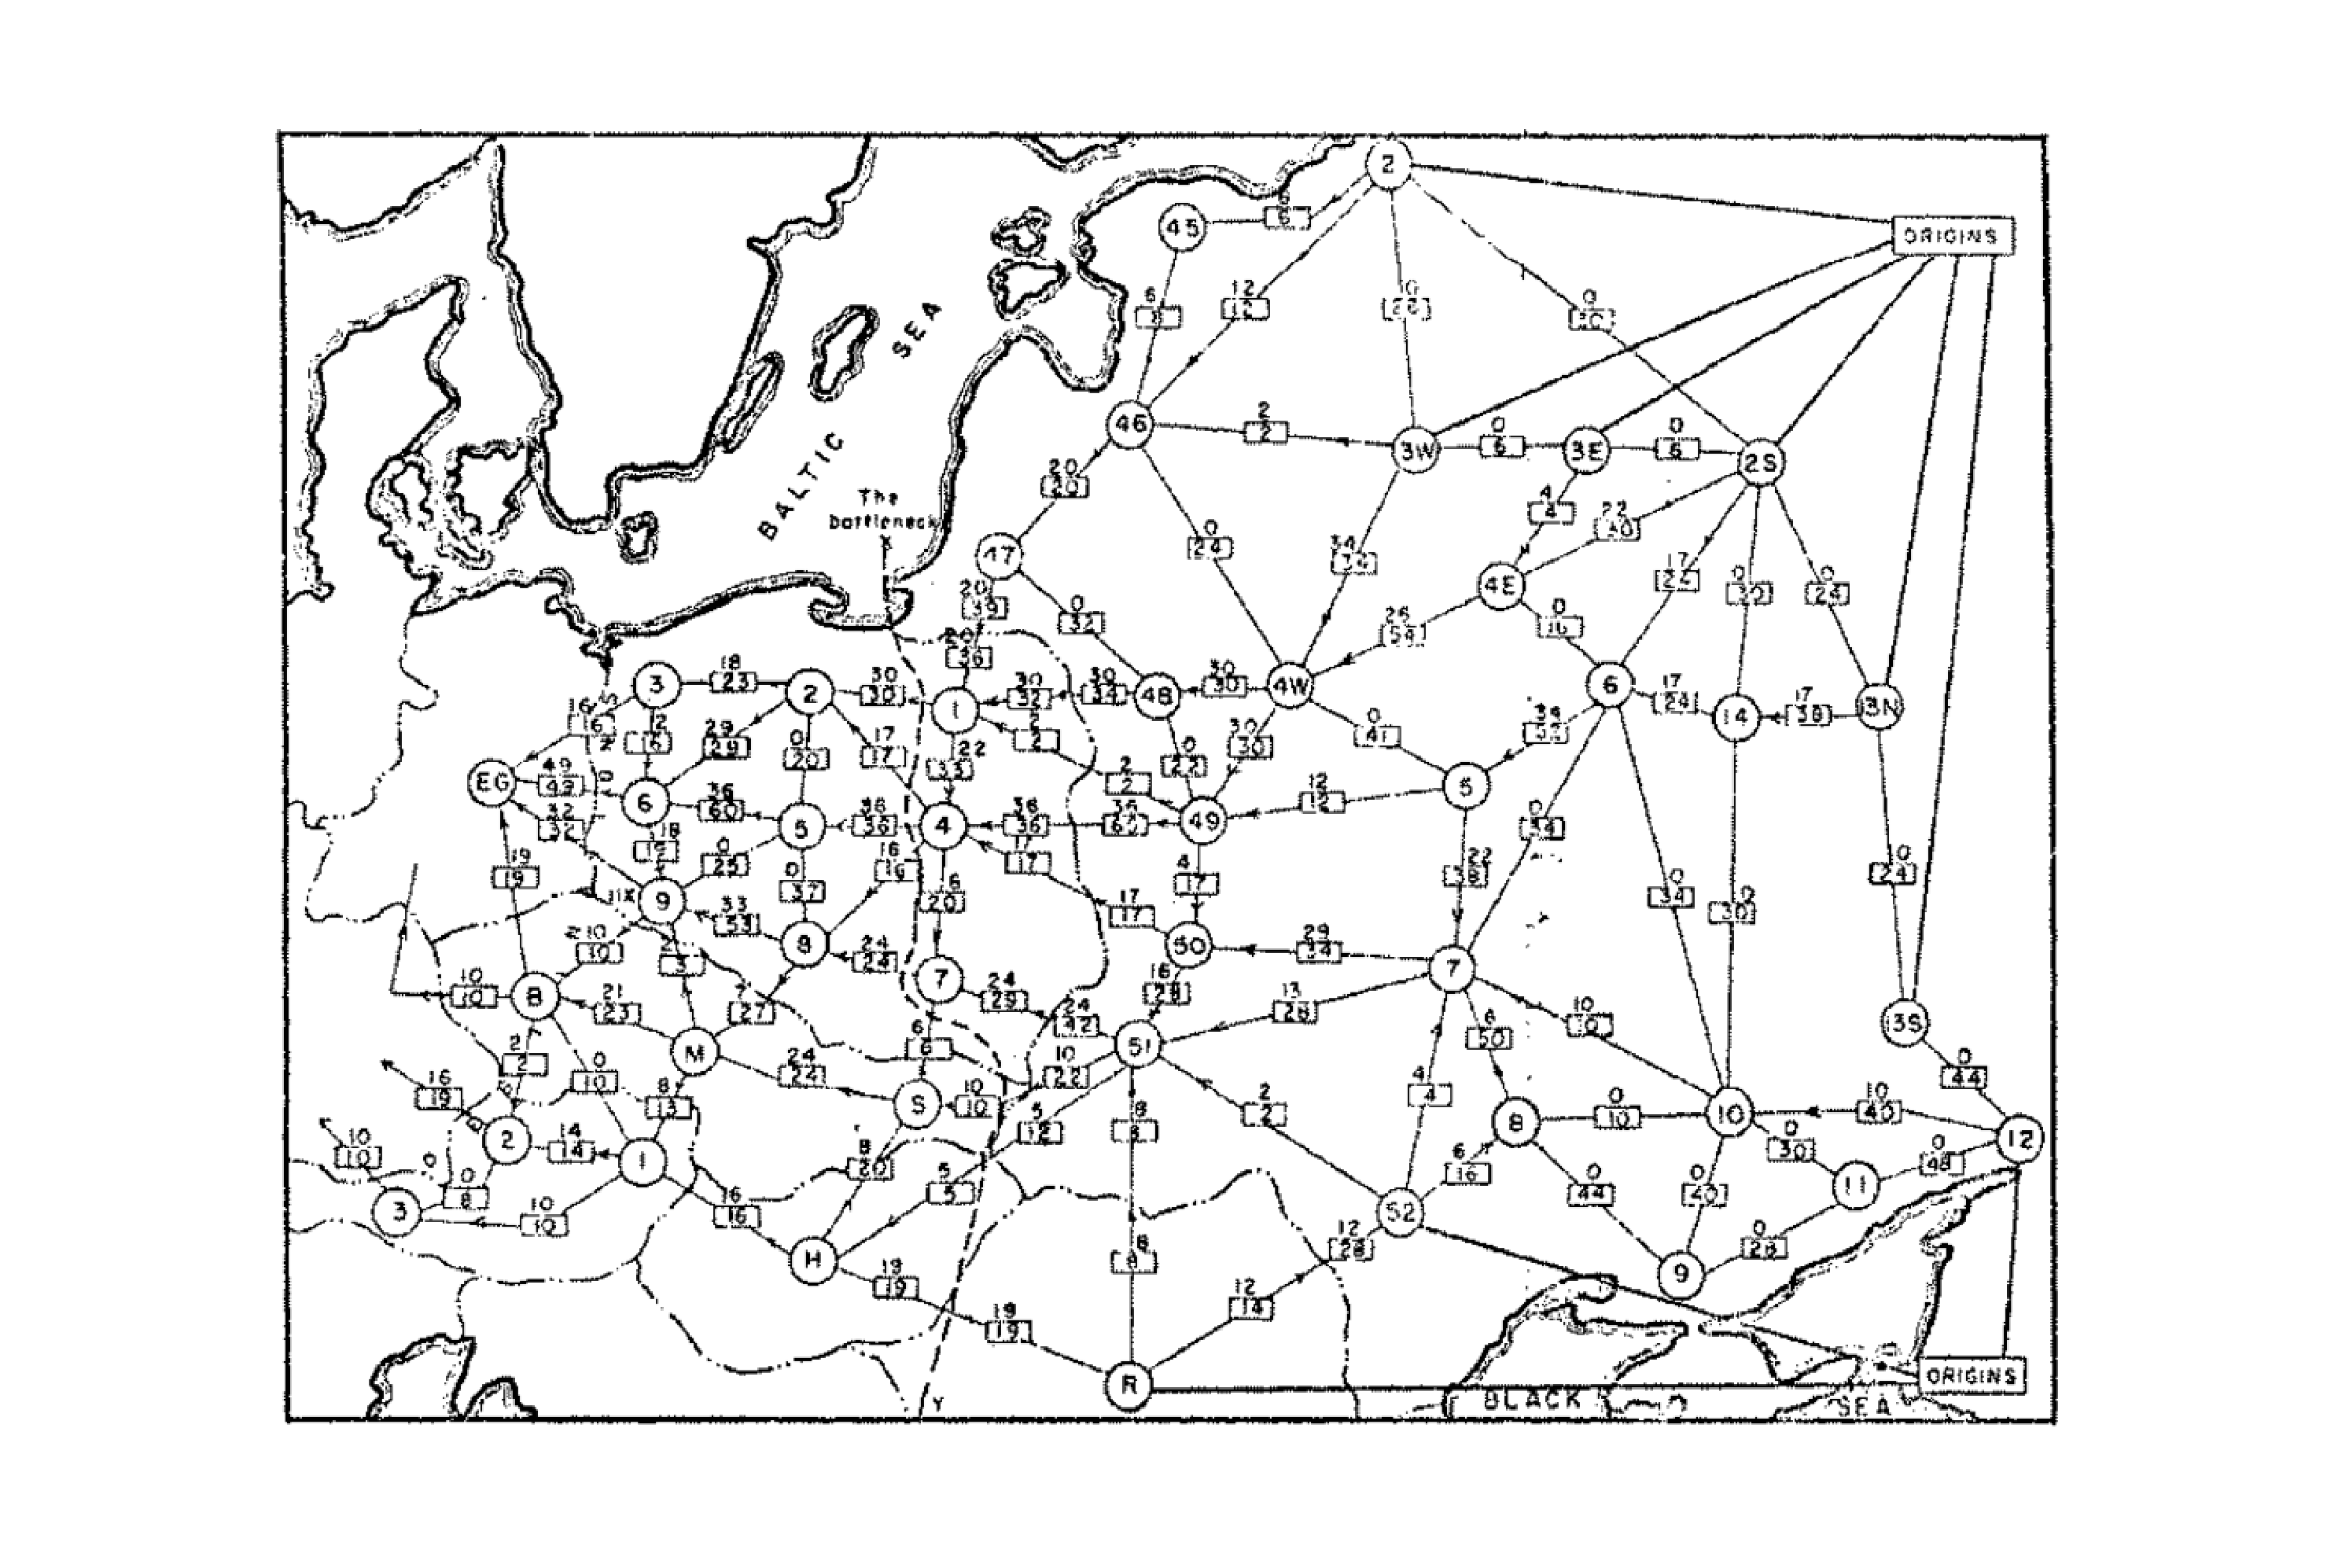
\includegraphics[width=3.5in] {L10-sovietunion.eps}
 \caption{Soviet Railway network, 1955}
\end{figure}
…… 1955年,美国开始在想,如何轰炸铁路,来阻断苏联同社会主义国家之间的联系。……
\begin{itemize}
 \item
\textit{``.... From Harris and Ross [1955]: Schematic diagram of the railway network of the Western
Soviet Union and Eastern European countries, with a maximum flow of value 163,000 tons
from Russia to Eastern Europe, and a cut of capacity 163,000 tons indicated as “The
bottleneck”. ....''}

\item
\textit{A recently declassified U.S. Air Force report indicates that the original motivation of minimum-cut problem and Ford-Fulkerson algorithm is \textcolor{red}{ to disrupt rail transportation the Soviet Union} [A. Shrijver, 2002].(2002年的解密文档) }
\end{itemize}
1955年提出的问题,到了1956年,Ford and Fulkerson就给了一个算法。从这个事情中又能够体现着出这件事情:原始问题的实际问题是什么,数学的抽象-建模是第二部,第三步是算法设计。

\begin{table}[H]
   {\begin{tabular}{lcc}\hline
%        & \multicolumn{3}{c}{Actual number of DCJ operations}\\
        Year  & Developers &  Time-complexity  \\
\hline
1956 & Ford and Fulkerson & $O(m C)$ and $O(m^2\log C)$ \\
1972 & Edmonds and Karp & $O(m^2 n)$ \\
1970 & Dinitz & $O(n^2 m)$ \\
1974 & Karzanov & $O(n^3)$ \\
1983 & Sleator and Tarjan & $O(nm \log n)$ \\
1988 & Goldberg and Tarjan & $O(n^2 m \log(\frac{n^{2}}{m}))$ \\
2012  & Orlin	& $O(nm)$ \\ \hline

     \end{tabular}} {}%
 \end{table}
\subsection{最大流问题}


\textbf{问题描述}
\begin{itemize}

\item 输入:
  一个有向图 $G=<V, E>$.每个顶点v表示一个城市,每条边e表示城市之间的路,每条边$e$有个容量限制$C_e$. 两个特殊的点:起点\textcolor{red}{\bf source} $s$ 和终点 \textcolor{red}{\bf sink} $t$;
\item 输出:
 对于每一条边 $e=(u, v)$, 分给一条流$f(u, v)$ 最终使得$\sum_{u, (s,u)\in E} f{(s,u)}$ 最大.
\end{itemize}

具体举例如下:
\begin{figure}[H]
\begin{tikzpicture}[scale=1.3, auto,swap]
    % Draw a 7,11 network
    % First we draw the vertices
    \foreach \pos/\name in {{(0,0)/s}, {(2,1)/u}, {(2,-1)/v},
                            {(4,0)/t}}
        \node[middlevertex, draw,  fill=blue!20] (\name) at \pos {$\name$};
    % Connect vertices with edges and draw weights
    \foreach \source/ \dest /\weight in {s/u/{c_1=2}, u/t/{ c_4=2},u/v/{c_3=3},s/v/{c_2=1},      v/t/{c_5=1} }
        \path[edge, sloped, midway, below, allow upside down] (\source) -- node[weight] {$\weight$} (\dest);
   \end{tikzpicture}
\end{figure}
目标:从s点运尽量多的货物到目的地t。

\begin{figure}[H]
\begin{tikzpicture}[scale=1.3, auto,swap]
    % Draw a 7,11 network
    % First we draw the vertices
    % Connect vertices with edges and draw weights
    \foreach \source/ \dest /\weight in {s/u/{1/2}, u/t/{ 0/2},u/v/{1/3},s/v/{0/1},      v/t/{1/1} }
        \path[edge, sloped, midway, below, allow upside down] (\source) -- node[weight] {$\weight$} (\dest);
    \path[draw, thick, ->, blue] (0, 0) -- (2,1);
         \path[draw, thick, ->, blue] (2,1) -- (2,-1);
             \path[draw, thick, ->, blue] (2, -1) -- (4, 0);
    \foreach \pos/\name in {{(0,0)/s}, {(2,1)/u}, {(2,-1)/v},
                            {(4,0)/t}}
        \node[middlevertex, draw,  fill=blue!20] (\name) at \pos {$\name$};

   \end{tikzpicture}
\end{figure}


\textbf{定义:flow}

$f: E\rightarrow R^+$ 是一个 \textcolor{red}{\bf $s-t$ flow} 如果:
\begin{enumerate}
 \item   (Capacity constraints): $0\leq f(e) \leq C_e$ 对于全部的 $e$成立;
 \item   (Conservation constraints): 对于任何中间节点$v \in V-\{s,t\}$, $f^{in}(v) = f^{out}(v)$, 其中 $f^{in}(v) = \sum_{e \text{  into } v} f(e) $ 并且 $f^{out}(v) = \sum_{ e \text{ out of } v} f(e)$. (直观: 输入 = 输出 对于任何节点.)
\end{enumerate}
 \textcolor{red}{\bf flow 的值 $f$}被定义为 $V(f) = f^{out}(s)$.


\textbf{定义:$s-t$ cut}

一个 \textcolor{red} {\bf $s-t$ cut}是一个划分 $V$ 的$(A,B)$ 从而使得 $s\in A$ and $t \in B$.
\textcolor{red}{\bf 割 cut $(A,B)$的capacity} 被定义为 $C(A,B) = \sum_{e \text{ from } A \text{ to } B} C(e)$.

\begin{figure}[H]
\begin{tikzpicture}[scale=1.3, auto,swap]
    % Draw a 7,11 network
    % First we draw the vertices

    % Connect vertices with edges and draw weights
    \foreach \source/ \dest /\weight in {s/u/{c_1=2}, u/t/{ c_4=2},u/v/{c_3=3},s/v/{c_2=1},      v/t/{c_5=1} }
        \path[edge, sloped, midway, below, allow upside down] (\source) -- node[weight] {$\weight$} (\dest);

        \path[draw, thick, white, ->] (0,0)--(2,1);
        \path[draw, thick, white, ->] (2,-1)--(4,0);
        \path[draw, thick, green, ->] (0,0)--(2,1);
        \path[draw, thick, green, ->] (2,-1)--(4,0);
         \node[below, red] at (0, -0.5) {$\mathbf{A}$};
         \node[above, red] at (4, 0.5) {$\mathbf{B}$};
         \path[draw, thick, dashed, red] (0.5,0.75)--(3.5,-0.75);
            \foreach \pos/\name in {{(0,0)/s}, {(2,1)/u}, {(2,-1)/v},{(4,0)/t}}
        \node[middlevertex, draw,  fill=blue!20] (\name) at \pos {$\name$};

   \end{tikzpicture}
\end{figure}
\begin{center}
$C(A, B) = 3$,只计从A到B的,不计从B到A的
\end{center}

\textbf{定义:流值引理}

给定一个流  $f$. 对于 \textcolor{red}{\bf 任何}  $s-t$ 割 cut $(A,B)$, 通过这个割的流是一个常量$V(f)$. 通常,  $V(f) = f^{out}( A ) - f^{in} (A)$.

\begin{figure}[H]
\begin{tikzpicture}[scale=1.3, auto,swap]
    % Draw a 7,11 network
    % First we draw the vertices

    % Connect vertices with edges and draw weights
    \foreach \source/ \dest /\weight in {s/u/{2/2}, u/t/{ 1/2},u/v/{1/3},s/v/{0/1},      v/t/{1/1} }
        \path[edge, sloped, midway, below, allow upside down] (\source) -- node[weight] {$\weight$} (\dest);

        \path[draw, thick, green, ->] (0,0)--(2,1);
        \path[draw, thick, green, ->] (2,-1)--(4,0);
        \path[draw, thick, blue, ->] (2,1)--(2,-1);
        \path[draw, thick, dashed, red] (0.5, 0.5)--(0.5, -0.6);
         \node[below, red] at (0, -0.5) {$\mathbf{A}$};
         \node[above, red] at (4, 0.5) {$\mathbf{B}$};
         \path[draw, thick, dashed, red] (0.5,0.75)--(3.5,-0.75);
            \foreach \pos/\name in {{(0,0)/s}, {(2,1)/u}, {(2,-1)/v},{(4,0)/t}}
        \node[middlevertex, draw,  fill=blue!20] (\name) at \pos {$\name$};

   \end{tikzpicture}
\end{figure}
\begin{center}
$V(f) = 2 + 0 = 2$\\
$f^{out}(A) - f^{in}(A) = 2 + 1 - 1 = V(f)$
\end{center}

\begin{figure}[H]
\begin{tikzpicture}[scale=1.3]
    % Draw a 7,11 network
    % First we draw the vertices

    % Connect vertices with edges and draw weights
    \foreach \source/ \dest /\weight in {s/u/{2/2}, u/t/{ 1/2},u/v/{1/3},s/v/{0/1},      v/t/{1/1} }
        \path[edge, sloped, midway, below, allow upside down] (\source) -- node[weight] {$\weight$} (\dest);
        \path[draw, thick, green, ->] (0,0)--(2,1);
        \path[draw, thick, green, ->] (2,-1)--(4,0);
        \path[draw, thick, blue, ->] (2,1)--(2,-1);
         \node[below, red] at (0, -0.5) {$\mathbf{A}$};
         \node[above, red] at (4, 0.5) {$\mathbf{B}$};
         \path[draw, thick, dashed, red] (0.5,0.75)--(3.5,-0.75);
                 \path[draw, thick, dashed, red] (0.5, 0.5)--(0.5, -0.6);
            \foreach \pos/\name in {{(0,0)/s}, {(2,1)/u}, {(2,-1)/v},{(4,0)/t}}
        \node[middlevertex, draw,  fill=blue!20] (\name) at \pos {$\name$};
   \end{tikzpicture}
\end{figure}

\textbf{引理证明}
\begin{small}
\begin{itemize}
\item  我们有: $0 = f^{out}(v) - f^{in}(v) $ 对于任何的 $v \neq s$ 和 $v \neq t$.这是条件。
\item  因此我们有:
\begin{eqnarray}
V(f) &=& f^{out}(s) - f^{in} (s)  \text{\qquad\qquad//提示: } f^{in}(s) = 0;\nonumber \\
     &=&  \sum\nolimits_{v \in A} ( f^{out}(v) - f^{in}(v) ) \nonumber \\
     &=&\ ( \sum\nolimits_{\text{ e from A to B}} f(e) + \sum\nolimits_{\text{ e from A to A}} f(e) )  \nonumber \\
     & &-( \sum\nolimits_{\text{ e from B to  A}} f(e) + \sum\nolimits_{\text{ e  from A to A }} f(e) ) \nonumber \\
     &=&  f^{out}(A) - f^{in} (A) \nonumber
\end{eqnarray}
\end{itemize}
\end{small}

以上是一些定义和引理。现在回到原问题。依据我们现在所学的知识,采用什么方法使得流最大。贪心可以,但肯定不太好,分支特别多,不是一个太好的选择。线性规划肯定可以,是万能的。首先这个问题不好分,是图的问题,不好规约。下面看一下1956年的Ford-Fulkerson algorithm 。

\subsection{Ford-Fulkerson algorithm}

\textbf{Lester Randolph Ford Jr. 和 Delbert Ray Fulkerson}

 \begin{figure}[H]%
   \begin{center}%
     \begin{minipage}{0.40\textwidth}%
      \includegraphics[width=1.0\textwidth]{FordJr.png}%
     \end{minipage}%
     \qquad
     \begin{minipage}{0.40\textwidth}
      \includegraphics[width=1.0\textwidth]{Fulkerson.png}%
     \end{minipage}%
   \end{center}
   \caption{ Lester Randolph Ford Jr. and Delbert Ray Fulkerson}
 \end{figure}

\textbf{尝试1:动态规划技术}

\begin{itemize}
\item
动态规划似乎不太好用.
\item
实际上,当前不存在一个{\sc 最大流} 问题可以真正的被看做是属于动态规划问题.
 \item
我们知道 {\sc 最大流} 问题 是在 $\mathbf{P}$ 中因为它可以写成动态规划 (见 Lecture 8).
\item
然而, 网络结构存在它自己的属性使得能够有一个更有效的算法,非正式的称作 \textcolor{red}{\bf network simplex}, 等等.
\end{itemize}

\textbf{尝试2:{\sc 改进} 策略}

问题不好分,我们尝试改进的策略。


{\sc Improvement}$(f)$
\begin{algorithmic}[1]
\STATE $\mathbf{x=x_0}$; //starting from an initial solution;
\WHILE{ \texttt{TRUE} }
\STATE $\mathbf{x}=${\sc Improve}$(\mathbf{x})$; //move one step towards optimum;
\IF { {\sc Stopping}$(\mathbf{x, f})$ }
\STATE break;
\ENDIF
\ENDWHILE
\RETURN $\mathbf{x}$;
\end{algorithmic}


\textbf{迭代框架的三个关键问题}


三个问题:
\begin{enumerate}
\item 如何构建一个初始解?
	\begin{itemize}
	\item 对于 {\sc 最大流} 问题,  一个0-流可以通过通过设置$f(e)=0$得到,对于任意$e$.
	\item 很容验证h {\sc conservation} 和 {\sc capacity} 约束都被满足,对于0-流来说.
	\end{itemize}
\item 如何改进这个解决办法?
\item 何时停止?
\end{enumerate}

先看一个随便一想就能想到的办法。

 \begin{itemize}
 \item
假定$p$ 是一个在网络 $G$中的简单 ${s-t}$ path.

  \begin{algorithmic}[1]
    \STATE Initialize $f(e)=0$ for all $e$.
    \WHILE{there is an  $s-t$ path  in graph $G$}
    \STATE  \textcolor{red}{\bf arbitrarily} choose an $s-t$ path $p$ in $G$;
    \STATE $f = ${\sc augment}$(p, f)$;
    \ENDWHILE
    \RETURN{$f$};
  \end{algorithmic}
\end{itemize}

我们定义 $bottleneck(p, f)$ 作为 path $p$上边的最小capacity.

{\sc augment}$(p, f):$\\
  \begin{algorithmic}[1]
  \STATE Let $b=bottleneck(p, f);$
    \FOR{each edge $e=(u,v)$ $\in P$}
    \IF{$(u,v)$ is a forward edge}
    \STATE increase $f(u,v)$ by $b;$
    \ELSE
    \STATE decrease $f(u,v)$ by $b;$
    \ENDIF
    \ENDFOR
  \end{algorithmic}

这是一个失败的算法。\\

为什么会失败呢?

\begin{itemize}
 \item
我们从 0-流开始.
为了减小 $f$的值, 我们找到一条 $s-t$ path, 比如说 $p = s\rightarrow u  \rightarrow v$, 来运更多的商品
\item
这三条边上的流可以被增加$1$ 同时满足conservation和capacity限制.
\item
然而,我们不能发现一条$s-t$ path存在于 $G$ 中,使得 $f$ 增加更多(左半部分)即使最大流是$2$ (右半部分).

\end{itemize}


\begin{figure}[H]
\begin{tikzpicture}[scale=1, auto,swap]

    \def\dx{0};
    \def\dy{0};	

     \foreach \x/\y/\name in { 0/0/s, 2/1/u, 2/-1/v, 4/0/t}
        \node[middlevertex, draw,  fill=blue!20] (\name) at (\x+\dx, \y+\dy) {$\name$};


    \foreach \source/ \dest /\weight in {s/u/{1/1}}
        \path[edge, sloped, midway, above, allow upside down, blue] (\source) -- node[weight] {\small $\weight$} (\dest);

    \foreach \source/ \dest /\weight in {u/t/{0/1}}
        \path[edge, sloped, midway, above, allow upside down] (\source) -- node[weight] {\small $\weight$} (\dest);

    \foreach \source/ \dest /\weight in {u/v/{1/1}}
        \path[edge, sloped, midway, above, allow upside down, blue] (\source) -- node[weight] {\small $\weight$} (\dest);

    \foreach \source/ \dest /\weight in {v/t/{1/1}}
        \path[edge, sloped, midway, below, allow upside down, blue] (\source) -- node[weight] {\small $\weight$} (\dest);

    \foreach \source/ \dest /\weight in {s/v/{0/1}}
        \path[edge, sloped, midway, below, allow upside down] (\source) -- node[weight] {\small $\weight$} (\dest);
       \node[ultra thick, red, below] at (v.south) {$V(f)=1$};


    \def\dx{5};
    \def\dy{0};	

     \foreach \x/\y/\name in { 0/0/s, 2/1/u, 2/-1/v, 4/0/t}
        \node[middlevertex, draw,  fill=blue!20] (\name) at (\x+\dx, \y+\dy) {$\name$};


    \foreach \source/ \dest /\weight in {s/u/{1/1}}
        \path[edge, sloped, midway, above, allow upside down, blue] (\source) -- node[weight] {\small $\weight$} (\dest);

    \foreach \source/ \dest /\weight in {u/t/{1/1}}
        \path[edge, sloped, midway, above, allow upside down, blue] (\source) -- node[weight] {\small $\weight$} (\dest);

    \foreach \source/ \dest /\weight in {u/v/{0/1}}
        \path[edge, sloped, midway, above, allow upside down ] (\source) -- node[weight] {\small $\weight$} (\dest);

    \foreach \source/ \dest /\weight in {v/t/{1/1}}
        \path[edge, sloped, midway, below, allow upside down, blue] (\source) -- node[weight] {\small $\weight$} (\dest);

    \foreach \source/ \dest /\weight in {s/v/{1/1}}
        \path[edge, sloped, midway, below, allow upside down, blue] (\source) -- node[weight] {\small $\weight$} (\dest);

    \node[ultra thick, red, below] at (v.south) {$V(f)=2$};

   \end{tikzpicture}
\end{figure}

\textbf{ Ford-Fulkerson algorithm: \textcolor{red}{\bf ``复原undo''} 功能}

关键性观察:
\begin{itemize}
 \item
当构建一个流 $f$时, 调度商品可能会犯错, 即,有些边不应该用来运输商品. 举个例子, 图中的边 $u\rightarrow v$ 就不应该使用.

\begin{figure}[H]
\begin{tikzpicture}[scale=1, auto,swap]

    \def\dx{0};
    \def\dy{0};	

     \foreach \x/\y/\name in { 0/0/s, 2/1/u, 2/-1/v, 4/0/t}
        \node[middlevertex, draw,  fill=blue!20] (\name) at (\x+\dx, \y+\dy) {$\name$};


    \foreach \source/ \dest /\weight in {s/u/{1/1}}
        \path[edge, sloped, midway, above, allow upside down, blue] (\source) -- node[weight] {\small $\weight$} (\dest);

    \foreach \source/ \dest /\weight in {u/t/{0/1}}
        \path[edge, sloped, midway, above, allow upside down] (\source) -- node[weight] {\small $\weight$} (\dest);

    \foreach \source/ \dest /\weight in {u/v/{1/1}}
        \path[edge, sloped, midway, above, allow upside down, red] (\source) -- node[weight] {\small $\weight$} (\dest);

    \foreach \source/ \dest /\weight in {v/t/{1/1}}
        \path[edge, sloped, midway, below, allow upside down, blue] (\source) -- node[weight] {\small $\weight$} (\dest);

    \foreach \source/ \dest /\weight in {s/v/{0/1}}
        \path[edge, sloped, midway, below, allow upside down] (\source) -- node[weight] {\small $\weight$} (\dest);
       \node[ultra thick, red, below] at (v.south) {$V(f)=1$};


%    \def\dx{5};
%    \def\dy{0};	
%
%     \foreach \x/\y/\name in { 0/0/s, 2/1/u, 2/-1/v, 4/0/t}
%        \node[middlevertex, draw,  fill=blue!20] (\name) at (\x+\dx, \y+\dy) {$\name$};
%
%
%    \foreach \source/ \dest /\weight in {s/u/{1/1}}
%        \path[edge, sloped, midway, above, allow upside down, blue] (\source) -- node[weight] {\small $\weight$} (\dest);
%
%    \foreach \source/ \dest /\weight in {u/t/{1/1}}
%        \path[edge, sloped, midway, above, allow upside down, blue] (\source) -- node[weight] {\small $\weight$} (\dest);
%
%    \foreach \source/ \dest /\weight in {u/v/{0/1}}
%        \path[edge, sloped, midway, above, allow upside down ] (\source) -- node[weight] {\small $\weight$} (\dest);
%
%    \foreach \source/ \dest /\weight in {v/t/{1/1}}
%        \path[edge, sloped, midway, below, allow upside down, blue] (\source) -- node[weight] {\small $\weight$} (\dest);
%
%    \foreach \source/ \dest /\weight in {s/v/{1/1}}
%        \path[edge, sloped, midway, below, allow upside down, blue] (\source) -- node[weight] {\small $\weight$} (\dest);
%
%    \node[ultra thick, red, below] at (v.south) {$V(f)=2$};

   \end{tikzpicture}
\end{figure}

 \item
  为了改进流$f$,我们应该使用一些手段 \textcolor{red}{\bf 更正在写错误}, 即 ``复原undo''边上做过的运输任务。
 \item 如何实现 "undo" 功能呢?
 \item   \textcolor{red}{\bf 增加反向边! }
 \item 假定我们增加一条 \textcolor{red}{\bf 反向} 边 $v\rightarrow u$ 到原始图. 接着我们可以更正这次运输,通过退回从$v$ 到 $u$的商品.
\end{itemize}


加了退货边的图就叫剩余图(Residual graph)。
\begin{figure}[H]
\begin{tikzpicture}[scale=1, auto,swap]

    \def\dx{0};
    \def\dy{0};	

     \foreach \x/\y/\name in { 0/0/s, 2/1/u, 2/-1/v, 4/0/t}
        \node[middlevertex, draw,  fill=blue!20] (\name) at (\x+\dx, \y+\dy) {$\name$};


    \foreach \source/ \dest /\weight in {s/u/{1/1}}
        \path[edge, sloped, midway, above, allow upside down, blue] (\source) -- node[weight] {\small $\weight$} (\dest);

    \foreach \source/ \dest /\weight in {u/t/{0/1}}
        \path[edge, sloped, midway, above, allow upside down] (\source) -- node[weight] {\small $\weight$} (\dest);

    \foreach \source/ \dest /\weight in {u/v/{1/1}}
        \path[edge, sloped, midway, above, allow upside down, blue] (\source) -- node[weight] {\small $\weight$} (\dest);

    \foreach \source/ \dest /\weight in {v/t/{1/1}}
        \path[edge, sloped, midway, below, allow upside down, blue] (\source) -- node[weight] {\small $\weight$} (\dest);

    \foreach \source/ \dest /\weight in {s/v/{0/1}}
        \path[edge, sloped, midway, below, allow upside down] (\source) -- node[weight] {\small $\weight$} (\dest);
       \node[ultra thick, blue, below] at (v.south) {Flow $f$};


    \def\dx{5};
    \def\dy{0};	

     \foreach \x/\y/\name in { 0/0/s, 2/1/u, 2/-1/v, 4/0/t}
        \node[middlevertex, draw,  fill=blue!20] (\name) at (\x+\dx, \y+\dy) {$\name$};

        \draw[->, thick] (s.15) -- node[below, sloped, midway] {\small $0$} (u.225);
        \draw[->, thick, red] (u.195) -- node[above, sloped, midway] {\small $1$} (s.45);

        \draw[->, thick] (u.285) -- node[above, sloped, midway] {\small $0$} (v.75);
        \draw[->, thick, red] (v.105) -- node[above, sloped, midway] {\small $1$} (u.255);

        \draw[->, thick] (v.15) -- node[below, sloped, midway] {\small $0$} (t.225);
        \draw[->, thick, red] (t.195) -- node[above, sloped, midway] {\small $1$} (v.45);


%    \foreach \source/ \dest /\weight in {s/u/{1/1}}
%        \path[edge, sloped, midway, above, allow upside down, blue] (\source) -- node[weight] {\small $\weight$} (\dest);

    \foreach \source/ \dest /\weight in {u/t/{1}}
        \path[edge, sloped, midway, above, allow upside down, black] (\source) -- node[weight] {\small $\weight$} (\dest);

%    \foreach \source/ \dest /\weight in {u/v/{0/1}}
%        \path[edge, sloped, midway, above, allow upside down ] (\source) -- node[weight] {\small $\weight$} (\dest);

%    \foreach \source/ \dest /\weight in {v/t/{1/1}}
%        \path[edge, sloped, midway, below, allow upside down, blue] (\source) -- node[weight] {\small $\weight$} (\dest);

    \foreach \source/ \dest /\weight in {s/v/{1}}
        \path[edge, sloped, midway, below, allow upside down, black] (\source) -- node[weight] {\small $\weight$} (\dest);

   \node[ultra thick, red, below] at (v.south) {Backward edges};

   \end{tikzpicture}
\end{figure}

\textbf{剩余图 Residual Graph}


   给定一个有向图$G=<V,E>$, 有一个流 $f$, 我们定义 \textcolor{red}{\bf 剩余图residual graph} $G_f=<V, E'>$. 对于任何一条边$e = (u,v) \in E$, 按照下面的要求将两条边加入到$E'$ :
\begin{enumerate}
\begin{small}
 \item (\textcolor{red}{\bf 正向边} $(u, v)$ 标注剩余的运输容量): \\
如果 $f(e) < C(e)$, 添加一条边$e=(u,v)$ 标注运输容量$C(e)=C(e) - f(e)$.
 \item (\textcolor{red}{\bf 反向边}  $(v, u)$ 标注回退容量): \\
如果 $f(e) > 0$, 添加一条边 $e'=(v,u)$ 标注回退容量 $C(e') = f(e)$.
\end{small}
\end{enumerate}

 \begin{figure}[H]
\begin{tikzpicture}[scale=1, auto,swap]

    \def\dx{0};
    \def\dy{0};	

     \foreach \x/\y/\name in { 0/0/s, 2/1/u, 2/-1/v, 4/0/t}
        \node[middlevertex, draw,  fill=blue!20] (\name) at (\x+\dx, \y+\dy) {$\name$};


    \foreach \source/ \dest /\weight in {s/u/{1/1}}
        \path[edge, sloped, midway, above, allow upside down, blue] (\source) -- node[weight] {\small $\weight$} (\dest);

    \foreach \source/ \dest /\weight in {u/t/{0/1}}
        \path[edge, sloped, midway, above, allow upside down] (\source) -- node[weight] {\small $\weight$} (\dest);

    \foreach \source/ \dest /\weight in {u/v/{1/1}}
        \path[edge, sloped, midway, above, allow upside down, blue] (\source) -- node[weight] {\small $\weight$} (\dest);

    \foreach \source/ \dest /\weight in {v/t/{1/1}}
        \path[edge, sloped, midway, below, allow upside down, blue] (\source) -- node[weight] {\small $\weight$} (\dest);

    \foreach \source/ \dest /\weight in {s/v/{0/1}}
        \path[edge, sloped, midway, below, allow upside down] (\source) -- node[weight] {\small $\weight$} (\dest);
       \node[ultra thick, blue, below] at (v.south) {Flow $f$};


    \def\dx{5};
    \def\dy{0};	

     \foreach \x/\y/\name in { 0/0/s, 2/1/u, 2/-1/v, 4/0/t}
        \node[middlevertex, draw,  fill=blue!20] (\name) at (\x+\dx, \y+\dy) {$\name$};

        \draw[->, thick] (s.15) -- node[below, sloped, midway] {\small $0$} (u.225);
        \draw[->, thick] (u.195) -- node[above, sloped, midway] {\small $1$} (s.45);

        \draw[->, thick] (u.285) -- node[above, sloped, midway] {\small $0$} (v.75);
        \draw[->, thick, green] (v.105) -- node[above, sloped, midway, green] {\small $1$} (u.255);

        \draw[->, thick] (v.15) -- node[below, sloped, midway] {\small $0$} (t.225);
        \draw[->, thick] (t.195) -- node[above, sloped, midway] {\small $1$} (v.45);


%    \foreach \source/ \dest /\weight in {s/u/{1/1}}
%        \path[edge, sloped, midway, above, allow upside down, blue] (\source) -- node[weight] {\small $\weight$} (\dest);

    \foreach \source/ \dest /\weight in {u/t/{1}}
        \path[edge, sloped, midway, above, allow upside down, green] (\source) -- node[weight] {\small $\weight$} (\dest);

%    \foreach \source/ \dest /\weight in {u/v/{0/1}}
%        \path[edge, sloped, midway, above, allow upside down ] (\source) -- node[weight] {\small $\weight$} (\dest);

%    \foreach \source/ \dest /\weight in {v/t/{1/1}}
%        \path[edge, sloped, midway, below, allow upside down, blue] (\source) -- node[weight] {\small $\weight$} (\dest);

    \foreach \source/ \dest /\weight in {s/v/{1}}
        \path[edge, sloped, midway, below, allow upside down, green] (\source) -- node[weight] {\small $\weight$} (\dest);

   \node[ultra thick, red, below] at (v.south) {Residual graph $G_f$};

   \end{tikzpicture}
\end{figure}
提示: 路径path中包含反向边 $(v,u)$。



\textbf{沿着路径增广流:从$f$ 到$f'$}
\begin{figure}[H]
\begin{tikzpicture}[scale=0.8, auto,swap]

    \def\dx{0};
    \def\dy{0};	

     \foreach \x/\y/\name in { 0/0/s, 2/1/u, 2/-1/v, 4/0/t}
        \node[middlevertex, draw,  fill=blue!20] (\name) at (\x+\dx, \y+\dy) {$\name$};


    \foreach \source/ \dest /\weight in {s/u/{1/1}}
        \path[edge, sloped, midway, above, allow upside down, blue] (\source) -- node[weight] {\small $\weight$} (\dest);

    \foreach \source/ \dest /\weight in {u/t/{0/1}}
        \path[edge, sloped, midway, above, allow upside down] (\source) -- node[weight] {\small $\weight$} (\dest);

    \foreach \source/ \dest /\weight in {u/v/{1/1}}
        \path[edge, sloped, midway, above, allow upside down, blue] (\source) -- node[weight] {\small $\weight$} (\dest);

    \foreach \source/ \dest /\weight in {v/t/{1/1}}
        \path[edge, sloped, midway, below, allow upside down, blue] (\source) -- node[weight] {\small $\weight$} (\dest);

    \foreach \source/ \dest /\weight in {s/v/{0/1}}
        \path[edge, sloped, midway, below, allow upside down] (\source) -- node[weight] {\small $\weight$} (\dest);
       \node[ultra thick, blue, below] at (v.south) {Flow $f$};

       \node[ultra thick, blue] at (4, -1.7 ) {\large +};

    \def\dx{5};
    \def\dy{0};	

     \foreach \x/\y/\name in { 0/0/s, 2/1/u, 2/-1/v, 4/0/t}
        \node[middlevertex, draw,  fill=blue!20] (\name) at (\x+\dx, \y+\dy) {$\name$};

        \draw[->, thick] (s.15) -- node[below, sloped, midway] {\small $0$} (u.225);
        \draw[->, thick] (u.195) -- node[above, sloped, midway] {\small $1$} (s.45);

        \draw[->, thick] (u.285) -- node[above, sloped, midway] {\small $0$} (v.75);
        \draw[->, thick, green] (v.105) -- node[above, sloped, midway, green] {\small $1$} (u.255);

        \draw[->, thick] (v.15) -- node[below, sloped, midway] {\small $0$} (t.225);
        \draw[->, thick] (t.195) -- node[above, sloped, midway] {\small $1$} (v.45);


%    \foreach \source/ \dest /\weight in {s/u/{1/1}}
%        \path[edge, sloped, midway, above, allow upside down, blue] (\source) -- node[weight] {\small $\weight$} (\dest);

    \foreach \source/ \dest /\weight in {u/t/{1}}
        \path[edge, sloped, midway, above, allow upside down, green] (\source) -- node[weight] {\small $\weight$} (\dest);

%    \foreach \source/ \dest /\weight in {u/v/{0/1}}
%        \path[edge, sloped, midway, above, allow upside down ] (\source) -- node[weight] {\small $\weight$} (\dest);

%    \foreach \source/ \dest /\weight in {v/t/{1/1}}
%        \path[edge, sloped, midway, below, allow upside down, blue] (\source) -- node[weight] {\small $\weight$} (\dest);

    \foreach \source/ \dest /\weight in {s/v/{1}}
        \path[edge, sloped, midway, below, allow upside down, green] (\source) -- node[weight] {\small $\weight$} (\dest);

   \node[ultra thick, green, below] at (v.south) {An $s-t$ path in $G_f$};


      \node[ultra thick, blue] at (10, -1.75) {\large =};


    \def\dx{10};
    \def\dy{0};	

     \foreach \x/\y/\name in { 0/0/s, 2/1/u, 2/-1/v, 4/0/t}
        \node[middlevertex, draw,  fill=blue!20] (\name) at (\x+\dx, \y+\dy) {$\name$};

%        \draw[->, thick] (s.15) -- node[below, sloped, midway] {\small $0$} (u.225);
%        \draw[->, thick] (u.195) -- node[above, sloped, midway] {\small $1$} (s.45);
%
%        \draw[->, thick] (u.285) -- node[above, sloped, midway] {\small $0$} (v.75);
%        \draw[->, thick, green] (v.105) -- node[above, sloped, midway, green] {\small $1$} (u.255);
%
%        \draw[->, thick] (v.15) -- node[below, sloped, midway] {\small $0$} (t.225);
%        \draw[->, thick] (t.195) -- node[above, sloped, midway] {\small $1$} (v.45);


    \foreach \source/ \dest /\weight in {s/u/{1/1}}
        \path[edge, sloped, midway, above, allow upside down, blue] (\source) -- node[weight] {\small $\weight$} (\dest);

    \foreach \source/ \dest /\weight in {u/t/{1/1}}
        \path[edge, sloped, midway, above, allow upside down, green] (\source) -- node[weight] {\small $\weight$} (\dest);

    \foreach \source/ \dest /\weight in {u/v/{0/1}}
        \path[edge, sloped, midway, above, allow upside down ] (\source) -- node[weight] {\small $\weight$} (\dest);

    \foreach \source/ \dest /\weight in {v/t/{1/1}}
        \path[edge, sloped, midway, below, allow upside down, blue] (\source) -- node[weight] {\small $\weight$} (\dest);

    \foreach \source/ \dest /\weight in {s/v/{1/1}}
        \path[edge, sloped, midway, below, allow upside down, green] (\source) -- node[weight] {\small $\weight$} (\dest);

   \node[ultra thick, red, below] at (v.south) {New flow $f'$};



   \end{tikzpicture}
\end{figure}

注释:

\begin{itemize}
\item
通过使用反向边 $v\rightarrow u$, 原始的从 $u$ 到 $v$的运输被退回.
\item 更具体的,
 第一次商品运输流$f$将会改变它的路径(从$s\rightarrow u\rightarrow v\rightarrow t$ 到 $s\rightarrow u\rightarrow t$),当第二次使用路 $s\rightarrow v\rightarrow t$的时候.
 \end{itemize}

  \subsection{求解最小割问题的算法的发展史}
  \begin{table}[h]
  \center
   {\begin{tabular}{lcc}\hline
%        & \multicolumn{3}{c}{Actual number of DCJ operations}\\
        年  & 提出者 &  时间复杂度  \\
\hline
1956 & Ford and Fulkerson & $O(m C)$ and $O(m^2\log C)$ \\
1972 & Edmonds and Karp & $O(m^2 n)$ \\
1970 & Dinitz & $O(n^2 m)$ \\
1974 & Karzanov & $O(n^3)$ \\
1983 & Sleator and Tarjan & $O(nm \log n)$ \\
1988 & Goldberg and Tarjan & $O(n^2 m \log(\frac{n^{2}}{m}))$ \\
2012  & Orlin	& $O(nm)$ \\ \hline

     \end{tabular}} {}%
 \end{table}
\subsection{最大流问题}
问题描述:有向图$G=<V,E>$,边$e$上有大小为$C_e$的容量限制,G中有两个特殊的点:起点s 和目的地t。 现给每条边$e=(u,v)$指定流值$f(u,v)$,问如何指定可使得总的流值$\sum_{u, (s,u)\in E} f{(s,u)}$ 最大。例如下图(图1.1):
\begin{figure}[H]
\center
\begin{tikzpicture}[scale=1.3, auto,swap]
    % Draw a 7,11 network
    % First we draw the vertices
    \foreach \pos/\name in {{(0,0)/s}, {(2,1)/u}, {(2,-1)/v},
                            {(4,0)/t}}
        \node[middlevertex, draw,  fill=blue!20] (\name) at \pos {$\name$};
    % Connect vertices with edges and draw weights
    \foreach \source/ \dest /\weight in {s/u/{c_1=2}, u/t/{ c_4=2},u/v/{c_3=3},s/v/{c_2=1},      v/t/{c_5=1} }
        \path[edge, sloped, midway, below, allow upside down] (\source) -- node[weight] {$\weight$} (\dest);
   \end{tikzpicture}
   \caption{图1.1 求解$s\rightarrow t$可运输的最多货物}
\end{figure}
目标:从起点s运输尽可能多的货物到目的地t。
\section{Ford-Fulkerson算法[1956]}
\begin{figure}[H]
   %\begin{center}
   \center
    % \begin{minipage}{0.40\textwidth}%
      \includegraphics[width=0.2\textwidth]{FordJr.png}%
     %\end{minipage}%
     \qquad
   %  \begin{minipage}{0.40\textwidth}
      \includegraphics[width=0.2\textwidth]{Fulkerson.png}%
     %\end{minipage}%
   %\end{center}
   \caption{Lester Randolph Ford Jr. and Delbert Ray Fulkerson}
 \end{figure}
 \subsection{动态规划求解}
 遗憾的是,该问题并不存在动态规划的多项式时间算法。但在第8节中也可以看出,该问题是P 类的,因为可以用线性规划求解。
 \subsection{Improvement策略}
 (1)Improvement策略大致思想\\
 先确定一个初始可行解,然后再改进,直到不能改进。该问题用Improve-
 ment 策略实现的伪代码如下:\\
{\sc Improvement}$(f)$
 \begin{algorithmic}[1]
\STATE $\mathbf{x=x_0}$; //starting from an initial solution;
\WHILE{ \texttt{TRUE} }
\STATE $\mathbf{x}=${\sc Improve}$(\mathbf{x})$; //move one step towards optimum;
\IF { {\sc Stopping}$(\mathbf{x, f})$ }
\STATE break;
\ENDIF
\ENDWHILE
\RETURN $\mathbf{x}$;
\end{algorithmic}

  (2)算法需要考虑的3个关键因素:\\
a.如何构造初始可行解? 一个很直接的方法是初始化为0流,每条边均有$f(e)=0$\\
b.如何对接进行改进\\
c.何时需要停止?

(3)一个失败的尝试\\
对于上节课所讲的一个笨拙的改进算法,随机选择可行流并在图上进行改进所得到的流,可能最终并不能终止于最优解。例如如下左图(图2.2)的可行流,该可行流无法通过增加流值再得到改进,但该可行流并不是最大流,因为右图(图2.3)是一个流值为2 的可行流。
\begin{figure}[H]
\center
\begin{tikzpicture}[scale=1, auto,swap]

    \def\dx{0};
    \def\dy{0};

     \foreach \x/\y/\name in { 0/0/s, 2/1/u, 2/-1/v, 4/0/t}
        \node[middlevertex, draw,  fill=blue!20] (\name) at (\x+\dx, \y+\dy) {$\name$};


    \foreach \source/ \dest /\weight in {s/u/{1/1}}
        \path[edge, sloped, midway, above, allow upside down, blue] (\source) -- node[weight] {\small $\weight$} (\dest);

    \foreach \source/ \dest /\weight in {u/t/{0/1}}
        \path[edge, sloped, midway, above, allow upside down] (\source) -- node[weight] {\small $\weight$} (\dest);

    \foreach \source/ \dest /\weight in {u/v/{1/1}}
        \path[edge, sloped, midway, above, allow upside down, blue] (\source) -- node[weight] {\small $\weight$} (\dest);

    \foreach \source/ \dest /\weight in {v/t/{1/1}}
        \path[edge, sloped, midway, below, allow upside down, blue] (\source) -- node[weight] {\small $\weight$} (\dest);

    \foreach \source/ \dest /\weight in {s/v/{0/1}}
        \path[edge, sloped, midway, below, allow upside down] (\source) -- node[weight] {\small $\weight$} (\dest);
       \node[ultra thick, below] at (v.south) {图2.2 $V(f)=1$};


    \def\dx{5};
    \def\dy{0};

     \foreach \x/\y/\name in { 0/0/s, 2/1/u, 2/-1/v, 4/0/t}
        \node[middlevertex, draw,  fill=blue!20] (\name) at (\x+\dx, \y+\dy) {$\name$};


    \foreach \source/ \dest /\weight in {s/u/{1/1}}
        \path[edge, sloped, midway, above, allow upside down, blue] (\source) -- node[weight] {\small $\weight$} (\dest);

    \foreach \source/ \dest /\weight in {u/t/{1/1}}
        \path[edge, sloped, midway, above, allow upside down, blue] (\source) -- node[weight] {\small $\weight$} (\dest);

    \foreach \source/ \dest /\weight in {u/v/{0/1}}
        \path[edge, sloped, midway, above, allow upside down ] (\source) -- node[weight] {\small $\weight$} (\dest);

    \foreach \source/ \dest /\weight in {v/t/{1/1}}
        \path[edge, sloped, midway, below, allow upside down, blue] (\source) -- node[weight] {\small $\weight$} (\dest);

    \foreach \source/ \dest /\weight in {s/v/{1/1}}
        \path[edge, sloped, midway, below, allow upside down, blue] (\source) -- node[weight] {\small $\weight$} (\dest);

    \node[ultra thick, below] at (v.south) {图2.3 $V(f)=2$};

   \end{tikzpicture}
\end{figure}

(4)Ford-Fulkerson算法引入反向边,让运出去的货物还可以有机会退回。将加入了退货边的图称为剩余图,构造剩余图的大致思路为,若$u\rightarrow v$运了$f$吨货物,且容量限制为$C(u,v)$,则剩余图中$u$到$v$ 的正向弧$u\rightarrow v$权值为$C(u,v)-f$,表示最多还可再运$C(u,v)-f$ 吨货,并构造权值为$f$的反向弧,表示最多可退大小为$f$的货物。例如,下面两个图分别代表网络的流图(图2.4)及剩余图(图2.5)。\\
\begin{figure}[H]
\center
\begin{tikzpicture}[scale=1, auto,swap]

    \def\dx{0};
    \def\dy{0};

     \foreach \x/\y/\name in { 0/0/s, 2/1/u, 2/-1/v, 4/0/t}
        \node[middlevertex, draw,  fill=blue!20] (\name) at (\x+\dx, \y+\dy) {$\name$};


    \foreach \source/ \dest /\weight in {s/u/{1/1}}
        \path[edge, sloped, midway, above, allow upside down, blue] (\source) -- node[weight] {\small $\weight$} (\dest);

    \foreach \source/ \dest /\weight in {u/t/{0/1}}
        \path[edge, sloped, midway, above, allow upside down] (\source) -- node[weight] {\small $\weight$} (\dest);

    \foreach \source/ \dest /\weight in {u/v/{1/1}}
        \path[edge, sloped, midway, above, allow upside down, blue] (\source) -- node[weight] {\small $\weight$} (\dest);

    \foreach \source/ \dest /\weight in {v/t/{1/1}}
        \path[edge, sloped, midway, below, allow upside down, blue] (\source) -- node[weight] {\small $\weight$} (\dest);

    \foreach \source/ \dest /\weight in {s/v/{0/1}}
        \path[edge, sloped, midway, below, allow upside down] (\source) -- node[weight] {\small $\weight$} (\dest);
       \node[ultra thick, below] at (v.south) {图2.4 Flow $f$};


    \def\dx{5};
    \def\dy{0};

     \foreach \x/\y/\name in { 0/0/s, 2/1/u, 2/-1/v, 4/0/t}
        \node[middlevertex, draw,  fill=blue!20] (\name) at (\x+\dx, \y+\dy) {$\name$};

        \draw[->, thick] (s.15) -- node[below, sloped, midway] {\small $0$} (u.225);
        \draw[->, thick, red] (u.195) -- node[above, sloped, midway] {\small $1$} (s.45);

        \draw[->, thick] (u.285) -- node[above, sloped, midway] {\small $0$} (v.75);
        \draw[->, thick, red] (v.105) -- node[above, sloped, midway] {\small $1$} (u.255);

        \draw[->, thick] (v.15) -- node[below, sloped, midway] {\small $0$} (t.225);
        \draw[->, thick, red] (t.195) -- node[above, sloped, midway] {\small $1$} (v.45);


%    \foreach \source/ \dest /\weight in {s/u/{1/1}}
%        \path[edge, sloped, midway, above, allow upside down, blue] (\source) -- node[weight] {\small $\weight$} (\dest);

    \foreach \source/ \dest /\weight in {u/t/{1}}
        \path[edge, sloped, midway, above, allow upside down, black] (\source) -- node[weight] {\small $\weight$} (\dest);

%    \foreach \source/ \dest /\weight in {u/v/{0/1}}
%        \path[edge, sloped, midway, above, allow upside down ] (\source) -- node[weight] {\small $\weight$} (\dest);

%    \foreach \source/ \dest /\weight in {v/t/{1/1}}
%        \path[edge, sloped, midway, below, allow upside down, blue] (\source) -- node[weight] {\small $\weight$} (\dest);

    \foreach \source/ \dest /\weight in {s/v/{1}}
        \path[edge, sloped, midway, below, allow upside down, black] (\source) -- node[weight] {\small $\weight$} (\dest);

   \node[ultra thick,  below] at (v.south) {图2.5 Backward edges};

   \end{tikzpicture}
\end{figure}

Ford-Fulkerson算法的实现过程可以简单地用如下所示的图来刻画:\\
\begin{figure}[h]
\center
\begin{tikzpicture}[scale=0.8, auto,swap]

    \def\dx{0};
    \def\dy{0};

     \foreach \x/\y/\name in { 0/0/s, 2/1/u, 2/-1/v, 4/0/t}
        \node[middlevertex, draw,  fill=blue!20] (\name) at (\x+\dx, \y+\dy) {$\name$};


    \foreach \source/ \dest /\weight in {s/u/{1/1}}
        \path[edge, sloped, midway, above, allow upside down, blue] (\source) -- node[weight] {\small $\weight$} (\dest);

    \foreach \source/ \dest /\weight in {u/t/{0/1}}
        \path[edge, sloped, midway, above, allow upside down] (\source) -- node[weight] {\small $\weight$} (\dest);

    \foreach \source/ \dest /\weight in {u/v/{1/1}}
        \path[edge, sloped, midway, above, allow upside down, blue] (\source) -- node[weight] {\small $\weight$} (\dest);

    \foreach \source/ \dest /\weight in {v/t/{1/1}}
        \path[edge, sloped, midway, below, allow upside down, blue] (\source) -- node[weight] {\small $\weight$} (\dest);

    \foreach \source/ \dest /\weight in {s/v/{0/1}}
        \path[edge, sloped, midway, below, allow upside down] (\source) -- node[weight] {\small $\weight$} (\dest);
       \node[ultra thick, blue, below] at (v.south) {Flow $f$};

       \node[ultra thick, blue] at (4, -1.7 ) {\large +};

    \def\dx{5};
    \def\dy{0};

     \foreach \x/\y/\name in { 0/0/s, 2/1/u, 2/-1/v, 4/0/t}
        \node[middlevertex, draw,  fill=blue!20] (\name) at (\x+\dx, \y+\dy) {$\name$};

        \draw[->, thick] (s.15) -- node[below, sloped, midway] {\small $0$} (u.225);
        \draw[->, thick] (u.195) -- node[above, sloped, midway] {\small $1$} (s.45);

        \draw[->, thick] (u.285) -- node[above, sloped, midway] {\small $0$} (v.75);
        \draw[->, thick, green] (v.105) -- node[above, sloped, midway, green] {\small $1$} (u.255);

        \draw[->, thick] (v.15) -- node[below, sloped, midway] {\small $0$} (t.225);
        \draw[->, thick] (t.195) -- node[above, sloped, midway] {\small $1$} (v.45);


%    \foreach \source/ \dest /\weight in {s/u/{1/1}}
%        \path[edge, sloped, midway, above, allow upside down, blue] (\source) -- node[weight] {\small $\weight$} (\dest);

    \foreach \source/ \dest /\weight in {u/t/{1}}
        \path[edge, sloped, midway, above, allow upside down, green] (\source) -- node[weight] {\small $\weight$} (\dest);

%    \foreach \source/ \dest /\weight in {u/v/{0/1}}
%        \path[edge, sloped, midway, above, allow upside down ] (\source) -- node[weight] {\small $\weight$} (\dest);

%    \foreach \source/ \dest /\weight in {v/t/{1/1}}
%        \path[edge, sloped, midway, below, allow upside down, blue] (\source) -- node[weight] {\small $\weight$} (\dest);

    \foreach \source/ \dest /\weight in {s/v/{1}}
        \path[edge, sloped, midway, below, allow upside down, green] (\source) -- node[weight] {\small $\weight$} (\dest);

   \node[ultra thick, green, below] at (v.south) {An $s-t$ path in $G_f$};


      \node[ultra thick, blue] at (10, -1.75) {\large =};


    \def\dx{10};
    \def\dy{0};

     \foreach \x/\y/\name in { 0/0/s, 2/1/u, 2/-1/v, 4/0/t}
        \node[middlevertex, draw,  fill=blue!20] (\name) at (\x+\dx, \y+\dy) {$\name$};

%        \draw[->, thick] (s.15) -- node[below, sloped, midway] {\small $0$} (u.225);
%        \draw[->, thick] (u.195) -- node[above, sloped, midway] {\small $1$} (s.45);
%
%        \draw[->, thick] (u.285) -- node[above, sloped, midway] {\small $0$} (v.75);
%        \draw[->, thick, green] (v.105) -- node[above, sloped, midway, green] {\small $1$} (u.255);
%
%        \draw[->, thick] (v.15) -- node[below, sloped, midway] {\small $0$} (t.225);
%        \draw[->, thick] (t.195) -- node[above, sloped, midway] {\small $1$} (v.45);


    \foreach \source/ \dest /\weight in {s/u/{1/1}}
        \path[edge, sloped, midway, above, allow upside down, blue] (\source) -- node[weight] {\small $\weight$} (\dest);

    \foreach \source/ \dest /\weight in {u/t/{1/1}}
        \path[edge, sloped, midway, above, allow upside down, green] (\source) -- node[weight] {\small $\weight$} (\dest);

    \foreach \source/ \dest /\weight in {u/v/{0/1}}
        \path[edge, sloped, midway, above, allow upside down ] (\source) -- node[weight] {\small $\weight$} (\dest);

    \foreach \source/ \dest /\weight in {v/t/{1/1}}
        \path[edge, sloped, midway, below, allow upside down, blue] (\source) -- node[weight] {\small $\weight$} (\dest);

    \foreach \source/ \dest /\weight in {s/v/{1/1}}
        \path[edge, sloped, midway, below, allow upside down, green] (\source) -- node[weight] {\small $\weight$} (\dest);

   \node[ultra thick, red, below] at (v.south) {New flow $f'$};



   \end{tikzpicture}
\end{figure}

简单来说,就是原始流 $+$ 剩余图中的可行路 $=$ 原始流的一个改进。\\
令$p$表示剩余图$G_f$中的一条简单路径,称为增广路径。并定义$bottleneck(p,f)$为路径$p$ 上的最小容量边。则Ford-Fulkerson算法可以描述为:\\
{\sc Ford-Fulkerson} algorithm
  \begin{algorithmic}[1]
    \STATE Initialize $f(e)=0$ for all $e$.
    \WHILE{there is an  $s-t$ path  in residual graph $G_f$}
    \STATE  \textcolor{red}{\bf arbitrarily} choose an $s-t$ path $p$ in $G_f$;
    \STATE $f = ${\sc augment}$(p, f)$;
    \ENDWHILE
    \RETURN{$f$};
  \end{algorithmic}

  与上节课所讲的随机行走的算法的唯一区别是剩余图有起点到终点的路而不是原网络图有起点到终点的路径。但这一小小的修改却可以使算法最终终止于最优解(网络的最大流)。

  下面是一个Ford-Fulkerson算法的实现。

\begin{figure}[H]
\center
\begin{tikzpicture} [scale=1.0, auto , swap]
  %\foreach \pos /\name in {{(0,0)/s},{()}}
  \node[ultra thick, below] at (4.5,3.5) {Ford-Fulkerson算法实例};
  \node[ultra thick, below] at (-1,2) {图G};
  \foreach \pos/\name in {{(0,0)/s}, {(3,2)/2}, {(3,0)/3},{(6,2)/4},{(6,0)/5},
                            {(9,0)/t}}
        \node[middlevertex, draw , fill=blue!20] (\name) at \pos {$\name$};
%    % Connect vertices with edges and draw weights
    \foreach \source/ \dest /\weight in {s/2/{10}, s/3/{10}, 2/3/{2},2/5/{8},      3/5/{9},2/4/{4},5/4/{6},4/t/{10},5/t/{10} }
     \path[edge, sloped, midway, above, allow upside down] (\source) -- node[weight] {$\weight$} (\dest);
    % \draw [->](8.7,1.8)--(7.6,1.5);
    % \draw[->](8.7,1.3)--(8,1);
     \node[ultra thick, below] at (t.south) {Flow $value = 0$};
\end{tikzpicture}
\end{figure}



%\begin{center}
%Step 1
%\end{center}

\begin{figure}[H]
\center
\begin{tikzpicture} [scale=1.0, auto , swap]
   \node[ultra thick , above] at (6.5,3){step1};
   \def\dx{0};
    \def\dy{0};
     \node[ultra thick, below] at (-1,1) {G};
     \foreach \x/\y/\name in { 0/0/s, 2/2/2, 2/0/3, 4/2/4, 4/0/5, 6/0/t}
        \node[middlevertex, draw,  fill=blue!20] (\name) at (\x+\dx, \y+\dy) {$\name$};

    \foreach \source/ \dest /\weight in {s/2/{0/10}}
        \path[edge, sloped, midway, above, allow upside down] (\source) -- node[weight] {\small $\weight$} (\dest);

    \foreach \source/ \dest /\weight in {2/3/{0/2}}
        \path[edge, sloped, midway, above, allow upside down] (\source) -- node[weight] {\small $\weight$} (\dest);
     \foreach \source/ \dest /\weight in {s/3/{0/10}}
        \path[edge, sloped, midway, below, allow upside down] (\source) -- node[weight] {\small $\weight$} (\dest);
     \foreach \source/ \dest /\weight in {2/4/{0/4}}
        \path[edge, sloped, midway, above, allow upside down] (\source) -- node[weight] {\small $\weight$} (\dest);
     \foreach \source/ \dest /\weight in {2/5/{0/8}}
        \path[edge, sloped, midway, above, allow upside down] (\source) -- node[weight] {\small $\weight$} (\dest);
     \foreach \source/ \dest /\weight in {3/5/{0/9}}
        \path[edge, sloped, midway, below, allow upside down] (\source) -- node[weight] {\small $\weight$} (\dest);
     \foreach \source/ \dest /\weight in {5/4/{0/10}}
        \path[edge, sloped, midway, below , allow upside down] (\source) -- node[weight] {\small $\weight$} (\dest);
     \foreach \source/ \dest /\weight in {4/t/{0/10}}
        \path[edge, sloped, midway, above, allow upside down] (\source) -- node[weight] {\small $\weight$} (\dest);
     \foreach \source/ \dest /\weight in {5/t/{0/10}}
        \path[edge, sloped, midway, below, allow upside down] (\source) -- node[weight] {\small $\weight$} (\dest);
     \node[ultra thick, below] at (t.south) {Flow value $=0$};


    \def\dx{8};
    \def\dy{0};
     \node[ultra thick, below] at (8,1){$G_f$};

     \foreach \x/\y/\name in { 0/0/s, 2/2/2, 2/0/3, 4/2/4, 4/0/5, 6/0/t}
        \node[middlevertex, draw,  fill=blue!20] (\name) at (\x+\dx, \y+\dy) {$\name$};

    \foreach \source/ \dest /\weight in {s/2/{10}}
        \path[edge, sloped, midway, above, allow upside down, red] (\source) -- node[weight] {\small $\weight$} (\dest);
    \foreach \source/ \dest /\weight in {s/3/{10}}
        \path[edge, sloped, midway, above, allow upside down] (\source) -- node[weight] {\small $\weight$} (\dest);
    \foreach \source/ \dest /\weight in {2/3/{2}}
        \path[edge, sloped, midway, above, allow upside down] (\source) -- node[weight] {\small $\weight$} (\dest);
    \foreach \source/ \dest /\weight in {2/4/{4}}
        \path[edge, sloped, midway, above, allow upside down] (\source) -- node[weight] {\small $\weight$} (\dest);
    \foreach \source/ \dest /\weight in {2/5/{8}}
        \path[edge, sloped, midway, above, allow upside down,red] (\source) -- node[weight] {\small $\weight$} (\dest);
    \foreach \source/ \dest /\weight in {3/5/{9}}
        \path[edge, sloped, midway, above, allow upside down] (\source) -- node[weight] {\small $\weight$} (\dest);
    \foreach \source/ \dest /\weight in {5/4/{6}}
        \path[edge, sloped, midway, above, allow upside down] (\source) -- node[weight] {\small $\weight$} (\dest);
    \foreach \source/ \dest /\weight in {4/t/{10}}
        \path[edge, sloped, midway, above, allow upside down] (\source) -- node[weight] {\small $\weight$} (\dest);
    \foreach \source/ \dest /\weight in {5/t/{10}}
        \path[edge, sloped, midway, above, allow upside down,red] (\source) -- node[weight] {\small $\weight$} (\dest);

\end{tikzpicture}
\end{figure}


%\begin{center}
%  step 2
%\end{center}
\begin{figure}[H]
\center
\begin{tikzpicture} [scale=1.0, auto , swap]

   \def\dx{0};
    \def\dy{0};
    \node[ultra thick, below] at (6.5,2.5) {step2};
     \node[ultra thick, below] at (-1,1) {G};
     \foreach \x/\y/\name in { 0/0/s, 2/2/2, 2/0/3, 4/2/4, 4/0/5, 6/0/t}
        \node[middlevertex, draw,  fill=blue!20] (\name) at (\x+\dx, \y+\dy) {$\name$};

    \foreach \source/ \dest /\weight in {s/2/{8/10}}
        \path[edge, sloped, midway, above, allow upside down] (\source) -- node[weight] {\small $\weight$} (\dest);

    \foreach \source/ \dest /\weight in {2/3/{0/2}}
        \path[edge, sloped, midway, above, allow upside down] (\source) -- node[weight] {\small $\weight$} (\dest);
     \foreach \source/ \dest /\weight in {s/3/{0/10}}
        \path[edge, sloped, midway, below, allow upside down] (\source) -- node[weight] {\small $\weight$} (\dest);
     \foreach \source/ \dest /\weight in {2/4/{0/4}}
        \path[edge, sloped, midway, above, allow upside down] (\source) -- node[weight] {\small $\weight$} (\dest);
     \foreach \source/ \dest /\weight in {2/5/{8/8}}
        \path[edge, sloped, midway, above, allow upside down] (\source) -- node[weight] {\small $\weight$} (\dest);
     \foreach \source/ \dest /\weight in {3/5/{0/9}}
        \path[edge, sloped, midway, below, allow upside down] (\source) -- node[weight] {\small $\weight$} (\dest);
     \foreach \source/ \dest /\weight in {5/4/{0/10}}
        \path[edge, sloped, midway, below , allow upside down] (\source) -- node[weight] {\small $\weight$} (\dest);
     \foreach \source/ \dest /\weight in {4/t/{0/10}}
        \path[edge, sloped, midway, above, allow upside down] (\source) -- node[weight] {\small $\weight$} (\dest);
     \foreach \source/ \dest /\weight in {5/t/{8/10}}
        \path[edge, sloped, midway, below, allow upside down] (\source) -- node[weight] {\small $\weight$} (\dest);
     \node[ultra thick, below] at (t.south) {Flow value $=8$};


    \def\dx{8};
    \def\dy{0};

       \node[ultra thick, below] at (8,1){$G_f$};

     \foreach \x/\y/\name in { 0/0/s, 2/2/2, 2/0/3, 4/2/4, 4/0/5, 6/0/t}
        \node[middlevertex, draw,  fill=blue!20] (\name) at (\x+\dx, \y+\dy) {$\name$};

    \draw[->, thick,red] (s.15) -- node[below, sloped, midway] {\small $2$} (2.225);
    \draw[->, thick] (2.195) -- node[above, sloped, midway] {\small $8$} (s.45);

    \foreach \source/ \dest /\weight in {s/3/{10}}
        \path[edge, sloped, midway, above, allow upside down] (\source) -- node[weight] {\small $\weight$} (\dest);
    \foreach \source/ \dest /\weight in {2/3/{2}}
        \path[edge, sloped, red,midway, above, allow upside down] (\source) -- node[weight] {\small $\weight$} (\dest);
    \foreach \source/ \dest /\weight in {2/4/{4}}
        \path[edge, sloped, midway, above, allow upside down] (\source) -- node[weight] {\small $\weight$} (\dest);
 \foreach \source/ \dest /\weight in {5/2/}
        \path[edge, sloped, midway, below, allow upside down] (\source) -- node[weight] {\small $\weight$} (\dest);
        \node[ultra thick] at(3.1+\dx,1+\dy){8};
    %\draw[->, thick] (2.325) -- node[above, sloped, midway] {\small $0$} (5.95);
%    \draw[->, thick] (5.135) -- node[below, sloped, midway] {\small $8$} (2.275);

    \foreach \source/ \dest /\weight in {3/5/{9}}
        \path[edge, sloped,red, midway, above, allow upside down] (\source) -- node[weight] {\small $\weight$} (\dest);
    \foreach \source/ \dest /\weight in {5/4/{6}}
        \path[edge, sloped, midway, above, allow upside down] (\source) -- node[weight] {\small $\weight$} (\dest);
    \foreach \source/ \dest /\weight in {4/t/{10}}
        \path[edge, sloped,midway, above, allow upside down] (\source) -- node[weight] {\small $\weight$} (\dest);
  \foreach \source/ \dest /\weight in {5/t/{2}}
        \path[edge, sloped,red,midway, above, allow upside down] (\source) -- node[weight] {\small $\weight$} (\dest);
   % \draw[->, thick] (5.53) -- node[above, sloped, midway] {\small $2$} (t);
    \draw[->, thick] (t.-825) -- node[below, sloped, midway] {\small $8$} (5.325);


\end{tikzpicture}
\end{figure}
%\begin{flushright} Flow value = 0\end{flushright}
%\end{frame}

\begin{figure}[H]
\center
\begin{tikzpicture} [scale=1.0, auto , swap]

   \def\dx{0};
    \def\dy{0};
    \node[ultra thick, below] at (6.5,2.5) {step3};
     \node[ultra thick, below] at (-1,1) {G};
     \foreach \x/\y/\name in { 0/0/s, 2/2/2, 2/0/3, 4/2/4, 4/0/5, 6/0/t}
        \node[middlevertex, draw,  fill=blue!20] (\name) at (\x+\dx, \y+\dy) {$\name$};

    \foreach \source/ \dest /\weight in {s/2/{10/10}}
        \path[edge, sloped, midway, above, allow upside down] (\source) -- node[weight] {\small $\weight$} (\dest);

    \foreach \source/ \dest /\weight in {2/3/{2/2}}
        \path[edge, sloped, midway, above, allow upside down] (\source) -- node[weight] {\small $\weight$} (\dest);
     \foreach \source/ \dest /\weight in {s/3/{0/10}}
        \path[edge, sloped, midway, below, allow upside down] (\source) -- node[weight] {\small $\weight$} (\dest);
     \foreach \source/ \dest /\weight in {2/4/{0/4}}
        \path[edge, sloped, midway, above, allow upside down] (\source) -- node[weight] {\small $\weight$} (\dest);
     \foreach \source/ \dest /\weight in {2/5/{8/8}}
        \path[edge, sloped, midway, above, allow upside down] (\source) -- node[weight] {\small $\weight$} (\dest);
     \foreach \source/ \dest /\weight in {3/5/{2/9}}
        \path[edge, sloped, midway, below, allow upside down] (\source) -- node[weight] {\small $\weight$} (\dest);
     \foreach \source/ \dest /\weight in {5/4/{0/10}}
        \path[edge, sloped, midway, below , allow upside down] (\source) -- node[weight] {\small $\weight$} (\dest);
     \foreach \source/ \dest /\weight in {4/t/{0/10}}
        \path[edge, sloped, midway, above, allow upside down] (\source) -- node[weight] {\small $\weight$} (\dest);
     \foreach \source/ \dest /\weight in {5/t/{10/10}}
        \path[edge, sloped, midway, below, allow upside down] (\source) -- node[weight] {\small $\weight$} (\dest);
     \node[ultra thick, below] at (t.south) {Flow value $=10$};


    \def\dx{8};
    \def\dy{0};
     \node[ultra thick ,below] at (0,1.5){$G_f$};
     \foreach \x/\y/\name in { 0/0/s, 2/2/2, 2/0/3, 4/2/4, 4/0/5, 6/0/t}
        \node[middlevertex, draw,  fill=blue!20] (\name) at (\x+\dx, \y+\dy) {$\name$};

   % \draw[->, thick] (s.15) -- node[below, sloped, midway] {\small $2$} (2.225);
   % \draw[->, thick] (2.195) -- node[above, sloped, midway] {\small $8$} (s.45);

    \foreach \source/ \dest /\weight in {2/s/}
        \path[edge, sloped, midway, above, allow upside down] (\source) -- node[weight] {\small $\weight$} (\dest);
    \node[ultra thick, below]at (1.1+\dx,1+\dy){10};

    \foreach \source/ \dest /\weight in {s/3/{10}}
        \path[edge, sloped, midway, above, allow upside down,red] (\source) -- node[weight] {\small $\weight$} (\dest);
    \foreach \source/ \dest /\weight in {3/2/{2}}
        \path[edge, sloped, midway, above, allow upside down] (\source) -- node[weight] {\small $\weight$} (\dest);
    \foreach \source/ \dest /\weight in {2/4/{4}}
        \path[edge, sloped, midway, above, allow upside down] (\source) -- node[weight] {\small $\weight$} (\dest);
     \foreach \source/ \dest /\weight in {5/2/{8}}
        \path[edge, sloped, midway, below, allow upside down] (\source) -- node[weight] {\small $\weight$} (\dest);
   % \draw[->, thick] (2.325) -- node[above, sloped, midway] {\small $0$} (5.95);
    %\draw[->, thick] (5.135) -- node[below, sloped, midway] {\small $8$} (2.275);

    \foreach \source/ \dest /\weight in {3/5/{7}}
        \path[edge, sloped, midway, above, allow upside down,red] (\source) -- node[weight] {\small $\weight$} (\dest);
    \draw[->,thick](5.-825)--node[below,sloped,midway]{\small $2$}(3.325);
    \foreach \source/ \dest /\weight in {5/4/{6}}
        \path[edge, sloped, midway, above, allow upside down,red] (\source) -- node[weight] {\small $\weight$} (\dest);
    \foreach \source/ \dest /\weight in {4/t/{10}}
        \path[edge, sloped,midway, above, allow upside down,red] (\source) -- node[weight] {\small $\weight$} (\dest);

    \foreach \source/ \dest /\weight in {t/5/}
        \path[edge, sloped, midway, above, allow upside down] (\source) -- node[weight] {\small $\weight$} (\dest);
        \node[ultra thick,above] at(5+\dx,-0.2+\dy) {10};

\end{tikzpicture}
\end{figure}

\begin{figure}[H]
\center
\begin{tikzpicture} [scale=1.0, auto , swap]

   \def\dx{0};
    \def\dy{0};
    \node[ultra thick, below] at (6.5,2.5) {step4};
     \node[ultra thick, below] at (-1,1) {G};
     \foreach \x/\y/\name in { 0/0/s, 2/2/2, 2/0/3, 4/2/4, 4/0/5, 6/0/t}
        \node[middlevertex, draw,  fill=blue!20] (\name) at (\x+\dx, \y+\dy) {$\name$};

    \foreach \source/ \dest /\weight in {s/2/{10/10}}
        \path[edge, sloped, midway, above, allow upside down] (\source) -- node[weight] {\small $\weight$} (\dest);

    \foreach \source/ \dest /\weight in {2/3/{2/2}}
        \path[edge, sloped, midway, above, allow upside down] (\source) -- node[weight] {\small $\weight$} (\dest);
     \foreach \source/ \dest /\weight in {s/3/{6/10}}
        \path[edge, sloped, midway, below, allow upside down] (\source) -- node[weight] {\small $\weight$} (\dest);
     \foreach \source/ \dest /\weight in {2/4/{0/4}}
        \path[edge, sloped, midway, above, allow upside down] (\source) -- node[weight] {\small $\weight$} (\dest);
     \foreach \source/ \dest /\weight in {2/5/{8/8}}
        \path[edge, sloped, midway, above, allow upside down] (\source) -- node[weight] {\small $\weight$} (\dest);
     \foreach \source/ \dest /\weight in {3/5/{8/9}}
        \path[edge, sloped, midway, below, allow upside down] (\source) -- node[weight] {\small $\weight$} (\dest);
     \foreach \source/ \dest /\weight in {5/4/{6/10}}
        \path[edge, sloped, midway, below , allow upside down] (\source) -- node[weight] {\small $\weight$} (\dest);
     \foreach \source/ \dest /\weight in {4/t/{6/10}}
        \path[edge, sloped, midway, above, allow upside down] (\source) -- node[weight] {\small $\weight$} (\dest);
     \foreach \source/ \dest /\weight in {5/t/{10/10}}
        \path[edge, sloped, midway, below, allow upside down] (\source) -- node[weight] {\small $\weight$} (\dest);
     \node[ultra thick, below] at (t.south) {Flow value $=16$};


    \def\dx{8};
    \def\dy{0};
     \node[ultra thick ,below] at (8,1.5){$G_f$};
     \foreach \x/\y/\name in { 0/0/s, 2/2/2, 2/0/3, 4/2/4, 4/0/5, 6/0/t}
        \node[middlevertex, draw,  fill=blue!20] (\name) at (\x+\dx, \y+\dy) {$\name$};

   % \draw[->, thick] (s.15) -- node[below, sloped, midway] {\small $2$} (2.225);
   % \draw[->, thick] (2.195) -- node[above, sloped, midway] {\small $8$} (s.45);

    \foreach \source/ \dest /\weight in {2/s/}
        \path[edge, sloped, midway, above, allow upside down] (\source) -- node[weight] {\small $\weight$} (\dest);
    \node[ultra thick, below]at (1+\dx,1+\dy){10};
    \foreach \source/ \dest /\weight in {3/2/{2}}
        \path[edge, sloped, midway, above, allow upside down,red] (\source) -- node[weight] {\small $\weight$} (\dest);
    \foreach \source/ \dest /\weight in {2/4/{4}}
        \path[edge, sloped, midway, above, allow upside down,red] (\source) -- node[weight] {\small $\weight$} (\dest);
     \foreach \source/ \dest /\weight in {5/2/{8}}
        \path[edge, sloped, midway, below, allow upside down] (\source) -- node[weight] {\small $\weight$} (\dest);
   % \draw[->, thick] (2.325) -- node[above, sloped, midway] {\small $0$} (5.95);
    %\draw[->, thick] (5.135) -- node[below, sloped, midway] {\small $8$} (2.275);

    \foreach \source/ \dest /\weight in {5/4/{6}}
        \path[edge, sloped, midway, above, allow upside down] (\source) -- node[weight] {\small $\weight$} (\dest);
    \foreach \source/ \dest /\weight in {4/t/{10}}
        \path[edge, sloped,midway, above, allow upside down,red] (\source) -- node[weight] {\small $\weight$} (\dest);

    \foreach \source/ \dest /\weight in {t/5/}
        \path[edge, sloped, midway, above, allow upside down] (\source) -- node[weight] {\small $\weight$} (\dest);
      \node[ultra thick, below] at (5+\dx,\dy) {10};

    \foreach \source/ \dest /\weight in {s/3/{4}}
        \path[edge, sloped, midway, above, allow upside down,red] (\source) -- node[weight] {\small $\weight$} (\dest);
    \draw[->,thick](3.-825)--node[below,sloped,midway]{\small $6$}(s.325);
    \foreach \source/ \dest /\weight in {3/5/{1}}
        \path[edge, sloped, midway, above, allow upside down] (\source) -- node[weight] {\small $\weight$} (\dest);
    \draw[->,thick](5.-825)--node[below,sloped,midway]{\small $8$}(3.325);
\end{tikzpicture}
\end{figure}

\begin{figure}[H]
\center
\begin{tikzpicture} [scale=1.0, auto , swap]

   \def\dx{0};
    \def\dy{0};
    \node[ultra thick, below] at (6.5,2.5) {step5};
     \node[ultra thick, below] at (-1,1) {G};
     \foreach \x/\y/\name in { 0/0/s, 2/2/2, 2/0/3, 4/2/4, 4/0/5, 6/0/t}
        \node[middlevertex, draw,  fill=blue!20] (\name) at (\x+\dx, \y+\dy) {$\name$};

    \foreach \source/ \dest /\weight in {s/2/{10/10}}
        \path[edge, sloped, midway, above, allow upside down] (\source) -- node[weight] {\small $\weight$} (\dest);

    \foreach \source/ \dest /\weight in {2/3/{0/2}}
        \path[edge, sloped, midway, above, allow upside down] (\source) -- node[weight] {\small $\weight$} (\dest);
     \foreach \source/ \dest /\weight in {s/3/{8/10}}
        \path[edge, sloped, midway, below, allow upside down] (\source) -- node[weight] {\small $\weight$} (\dest);
     \foreach \source/ \dest /\weight in {2/4/{2/4}}
        \path[edge, sloped, midway, above, allow upside down] (\source) -- node[weight] {\small $\weight$} (\dest);
     \foreach \source/ \dest /\weight in {2/5/{8/8}}
        \path[edge, sloped, midway, above, allow upside down] (\source) -- node[weight] {\small $\weight$} (\dest);
     \foreach \source/ \dest /\weight in {3/5/{8/9}}
        \path[edge, sloped, midway, below, allow upside down] (\source) -- node[weight] {\small $\weight$} (\dest);
     \foreach \source/ \dest /\weight in {5/4/{6/10}}
        \path[edge, sloped, midway, below , allow upside down] (\source) -- node[weight] {\small $\weight$} (\dest);
     \foreach \source/ \dest /\weight in {4/t/{8/10}}
        \path[edge, sloped, midway, above, allow upside down] (\source) -- node[weight] {\small $\weight$} (\dest);
     \foreach \source/ \dest /\weight in {5/t/{10/10}}
        \path[edge, sloped, midway, below, allow upside down] (\source) -- node[weight] {\small $\weight$} (\dest);
     \node[ultra thick, below] at (t.south) {Flow value $=18$};


    \def\dx{8};
    \def\dy{0};
     \node[ultra thick ,below] at (8,1.5){$G_f$};
     \foreach \x/\y/\name in { 0/0/s, 2/2/2, 2/0/3, 4/2/4, 4/0/5, 6/0/t}
        \node[middlevertex, draw,  fill=blue!20] (\name) at (\x+\dx, \y+\dy) {$\name$};

    %\draw[->, thick] (s.15) -- node[below, sloped, midway] {\small $2$} (2.225);
    %\draw[->, thick] (2.195) -- node[above, sloped, midway] {\small $8$} (s.45);

    \foreach \source/ \dest /\weight in {2/s/}
        \path[edge, sloped, midway, above, allow upside down] (\source) -- node[weight] {\small $\weight$} (\dest);
    \node[ultra thick,below] at (1+\dx,1+\dy) {10};

    \foreach \source/ \dest /\weight in {2/3/{2}}
        \path[edge, sloped, midway, above, allow upside down] (\source) -- node[weight] {\small $\weight$} (\dest);

    \foreach \source/ \dest /\weight in {2/4/{2}}
        \path[edge, sloped, midway, above, allow upside down,red] (\source) -- node[weight] {\small $\weight$} (\dest);
        \draw[->,thick](4.-825)--node[below,sloped,midway]{\small $8$}(2.325);

     \foreach \source/ \dest /\weight in {5/2/{8}}
        \path[edge, sloped, midway, below, allow upside down,red] (\source) -- node[weight] {\small $\weight$} (\dest);
   % \draw[->, thick] (2.325) -- node[above, sloped, midway] {\small $0$} (5.95);
    %\draw[->, thick] (5.135) -- node[below, sloped, midway] {\small $8$} (2.275);

    \foreach \source/ \dest /\weight in {4/5/{6}}
        \path[edge, sloped, midway, above, allow upside down] (\source) -- node[weight] {\small $\weight$} (\dest);
    \foreach \source/ \dest /\weight in {4/t/{2}}
        \path[edge, sloped,midway, above, allow upside down,red] (\source) -- node[weight] {\small $\weight$} (\dest);
    \draw [->,thick](t.90) arc [start angle=25, end angle=62, radius=4cm];
    \node[ultra thick,above]at(5.5+\dx,1+\dy){8};

    \foreach \source/ \dest /\weight in {t/5/{}}
        \path[edge, sloped, midway, above, allow upside down] (\source) -- node[weight] {\small $\weight$} (\dest);
      \node[ultra thick, below] at (5+\dx,\dy) {10};

    \foreach \source/ \dest /\weight in {3/s/}
        \path[edge, sloped, midway, above, allow upside down] (\source) -- node[weight] {\small $\weight$} (\dest);
    \node[ultra thick,above]at (1+\dx,\dy){8};
    %\draw[->,thick](3.-825)--node[below,sloped,midway]{\small $6$}(s.325);
    \draw [->,thick,red](s.-30) arc [start angle=250, end angle=280, radius=3.5cm];
   \node[ultra thick,above] at (1+\dx ,-0.8+\dy) {2};

    \foreach \source/ \dest /\weight in {5/3/}
        \path[edge, sloped, midway, above, allow upside down] (\source) -- node[weight] {\small $\weight$} (\dest);
        \node[ultra thick, below] at (3+\dx,0.1+\dy) {8};
    %\draw[->,thick](5.-825)--node[below,sloped,midway]{\small $8$}(3.325);
     \draw [->,thick,red](3.-30) arc [start angle=250, end angle=280, radius=3.5cm];
     \node[ultra thick,above] at (3+\dx ,-0.8+\dy) {1};
    %\draw[->, thick] (s.15) -- node[below, sloped, midway] {\small $2$} (2.225);
    %\draw[->, thick] (2.195) -- node[above, sloped, midway] {\small $8$} (s.45);

\end{tikzpicture}
\end{figure}

\begin{figure}[H]
\center
\begin{tikzpicture} [scale=1.0, auto , swap]

   \def\dx{0};
    \def\dy{0};
    \node[ultra thick, below] at (6.5,2.5) {step6};
     \node[ultra thick, below] at (-1,1) {G};
     \foreach \x/\y/\name in { 0/0/s, 2/2/2, 2/0/3, 4/2/4, 4/0/5, 6/0/t}
        \node[middlevertex, draw,  fill=blue!20] (\name) at (\x+\dx, \y+\dy) {$\name$};

    \foreach \source/ \dest /\weight in {s/2/{10/10}}
        \path[edge, sloped, midway, above, allow upside down] (\source) -- node[weight] {\small $\weight$} (\dest);

    \foreach \source/ \dest /\weight in {2/3/{0/2}}
        \path[edge, sloped, midway, above, allow upside down] (\source) -- node[weight] {\small $\weight$} (\dest);
     \foreach \source/ \dest /\weight in {s/3/{9/10}}
        \path[edge, sloped, midway, below, allow upside down] (\source) -- node[weight] {\small $\weight$} (\dest);
     \foreach \source/ \dest /\weight in {2/4/{3/4}}
        \path[edge, sloped, midway, above, allow upside down] (\source) -- node[weight] {\small $\weight$} (\dest);
     \foreach \source/ \dest /\weight in {2/5/{7/8}}
        \path[edge, sloped, midway, above, allow upside down] (\source) -- node[weight] {\small $\weight$} (\dest);
     \foreach \source/ \dest /\weight in {3/5/{9/9}}
        \path[edge, sloped, midway, below, allow upside down] (\source) -- node[weight] {\small $\weight$} (\dest);
     \foreach \source/ \dest /\weight in {5/4/{6/10}}
        \path[edge, sloped, midway, below , allow upside down] (\source) -- node[weight] {\small $\weight$} (\dest);
     \foreach \source/ \dest /\weight in {4/t/{9/10}}
        \path[edge, sloped, midway, above, allow upside down] (\source) -- node[weight] {\small $\weight$} (\dest);
     \foreach \source/ \dest /\weight in {5/t/{10/10}}
        \path[edge, sloped, midway, below, allow upside down] (\source) -- node[weight] {\small $\weight$} (\dest);
     \node[ultra thick, below] at (t.south) {Flow value $=19$};


    \def\dx{8};
    \def\dy{0};
     \node[ultra thick ,below] at (8,1.5){$G_f$};
     \foreach \x/\y/\name in { 0/0/s, 2/2/2, 2/0/3, 4/2/4, 4/0/5, 6/0/t}
        \node[middlevertex, draw,  fill=blue!20] (\name) at (\x+\dx, \y+\dy) {$\name$};

    %\draw[->, thick] (s.15) -- node[below, sloped, midway] {\small $2$} (2.225);
    %\draw[->, thick] (2.195) -- node[above, sloped, midway] {\small $8$} (s.45);

    \foreach \source/ \dest /\weight in {2/s/}
        \path[edge, sloped, midway, above, allow upside down] (\source) -- node[weight] {\small $\weight$} (\dest);
    \node[ultra thick,below] at (1+\dx,1+\dy) {10};

    \foreach \source/ \dest /\weight in {2/3/{2}}
        \path[edge, sloped, midway, above, allow upside down] (\source) -- node[weight] {\small $\weight$} (\dest);

    \foreach \source/ \dest /\weight in {2/4/{1}}
        \path[edge, sloped, midway, below, allow upside down] (\source) -- node[weight] {\small $\weight$} (\dest);
        %\draw[->,thick](4.-825)--node[below,sloped,midway]{\small $8$}(2.325);
        %4-->2  circle :value=3
        \draw [->,thick](4.120) arc [start angle=75, end angle=105, radius=3.5cm];
        \node[ultra thick, below] at (3+\dx,3+\dy){3};
     \foreach \source/ \dest /\weight in {2/5/{1}}
        \path[edge, sloped, midway, below, allow upside down] (\source) -- node[weight] {\small $\weight$} (\dest);
        \draw [->,thick](5.100) arc [start angle=33, end angle=63, radius=4.6cm];
        \node[ultra thick, above]at (3.2+\dx,1+\dy) {7};
   % \draw[->, thick] (2.325) -- node[above, sloped, midway] {\small $0$} (5.95);
    %\draw[->, thick] (5.135) -- node[below, sloped, midway] {\small $8$} (2.275);

    \foreach \source/ \dest /\weight in {4/5/}
        \path[edge, sloped, midway, above, allow upside down] (\source) -- node[weight] {\small $\weight$} (\dest);
        \node[ultra thick,above]at(4.1+\dx,1+\dy){6};
    \foreach \source/ \dest /\weight in {4/t/{1}}
        \path[edge, sloped,midway, above, allow upside down] (\source) -- node[weight] {\small $\weight$} (\dest);
    \draw [->,thick](t.100) arc [start angle=25, end angle=58, radius=4.5cm];
    \node[ultra thick,above]at(5.5+\dx,1+\dy){9};

    \foreach \source/ \dest /\weight in {t/5/{}}
        \path[edge, sloped, midway, above, allow upside down] (\source) -- node[weight] {\small $\weight$} (\dest);
      \node[ultra thick, below] at (5+\dx,\dy) {10};

    \foreach \source/ \dest /\weight in {3/s/}
        \path[edge, sloped, midway, below, allow upside down] (\source) -- node[weight] {\small $\weight$} (\dest);
    \node[ultra thick,below] at (1+\dx,0.4+\dy){9};
   \draw [->,thick](s.-30) arc [start angle=250, end angle=280, radius=3.5cm];
   \node[ultra thick,above] at (1+\dx ,-0.5+\dy) {1};
    %\draw[->,thick](3.-825)--node[below,sloped,midway]{\small $6$}(s.325);

    \foreach \source/ \dest /\weight in {5/3/{9}}
        \path[edge, sloped, midway, above, allow upside down] (\source) -- node[weight] {\small $\weight$} (\dest);
    %\draw[->,thick](5.-825)--node[below,sloped,midway]{\small $8$}(3.325);

    %\draw[->, thick] (s.15) -- node[below, sloped, midway] {\small $2$} (2.225);
    %\draw[->, thick] (2.195) -- node[above, sloped, midway] {\small $8$} (s.45);

\end{tikzpicture}
\end{figure}

\begin{figure}[H]
\center
\begin{tikzpicture} [scale=1.0, auto , swap]

   \def\dx{0};
    \def\dy{0};
    \node[ultra thick, below] at (6.5,2.5) {step7};

     \draw (1,0) ellipse [x radius=2cm,y radius=.5cm,fill=blue!20];


     \node[ultra thick, below] at (-1,1) {G};
     \foreach \x/\y/\name in { 0/0/s, 2/2/2, 2/0/3, 4/2/4, 4/0/5, 6/0/t}
        \node[middlevertex, draw,  fill=blue!20] (\name) at (\x+\dx, \y+\dy) {$\name$};

    \foreach \source/ \dest /\weight in {s/2/{10/10}}
        \path[edge, sloped, midway, above, allow upside down] (\source) -- node[weight] {\small $\weight$} (\dest);

    \foreach \source/ \dest /\weight in {2/3/{0/2}}
        \path[edge, sloped, midway, above, allow upside down] (\source) -- node[weight] {\small $\weight$} (\dest);
     \foreach \source/ \dest /\weight in {s/3/{9/10}}
        \path[edge, sloped, midway, below, allow upside down] (\source) -- node[weight] {\small $\weight$} (\dest);
     \foreach \source/ \dest /\weight in {2/4/{3/4}}
        \path[edge, sloped, midway, above, allow upside down] (\source) -- node[weight] {\small $\weight$} (\dest);
     \foreach \source/ \dest /\weight in {2/5/{7/8}}
        \path[edge, sloped, midway, above, allow upside down] (\source) -- node[weight] {\small $\weight$} (\dest);
     \foreach \source/ \dest /\weight in {3/5/{9/9}}
        \path[edge, sloped, midway, below, allow upside down] (\source) -- node[weight] {\small $\weight$} (\dest);
     \foreach \source/ \dest /\weight in {5/4/{6/10}}
        \path[edge, sloped, midway, below , allow upside down] (\source) -- node[weight] {\small $\weight$} (\dest);
     \foreach \source/ \dest /\weight in {4/t/{9/10}}
        \path[edge, sloped, midway, above, allow upside down] (\source) -- node[weight] {\small $\weight$} (\dest);
     \foreach \source/ \dest /\weight in {5/t/{10/10}}
        \path[edge, sloped, midway, below, allow upside down] (\source) -- node[weight] {\small $\weight$} (\dest);
     \node[ultra thick, below] at (t.south) {Flow value $=19$\quad cut capacity=$19$};


    \def\dx{8};
    \def\dy{0};

     \draw (1+\dx,0+\dy) ellipse [x radius=2cm,y radius=.5cm];

     \node[ultra thick ,below] at (8,1.5){$G_f$};
     \foreach \x/\y/\name in { 0/0/s, 2/2/2, 2/0/3, 4/2/4, 4/0/5, 6/0/t}
        \node[middlevertex, draw,  fill=blue!20] (\name) at (\x+\dx, \y+\dy) {$\name$};

    %\draw[->, thick] (s.15) -- node[below, sloped, midway] {\small $2$} (2.225);
    %\draw[->, thick] (2.195) -- node[above, sloped, midway] {\small $8$} (s.45);

    \foreach \source/ \dest /\weight in {2/s/}
        \path[edge, sloped, midway, above, allow upside down] (\source) -- node[weight] {\small $\weight$} (\dest);
    \node[ultra thick,below] at (1+\dx,1+\dy) {10};

    \foreach \source/ \dest /\weight in {2/3/{2}}
        \path[edge, sloped, midway, above, allow upside down] (\source) -- node[weight] {\small $\weight$} (\dest);

    \foreach \source/ \dest /\weight in {2/4/{1}}
        \path[edge, sloped, midway, below, allow upside down] (\source) -- node[weight] {\small $\weight$} (\dest);
        %\draw[->,thick](4.-825)--node[below,sloped,midway]{\small $8$}(2.325);
        %4-->2  circle :value=3
        \draw [->,thick](4.120) arc [start angle=75, end angle=105, radius=3.5cm];
        \node[ultra thick, below] at (3+\dx,3+\dy){3};
     \foreach \source/ \dest /\weight in {2/5/{1}}
        \path[edge, sloped, midway, below, allow upside down] (\source) -- node[weight] {\small $\weight$} (\dest);
        \draw [->,thick](5.100) arc [start angle=33, end angle=63, radius=4.6cm];
        \node[ultra thick, above]at (3.2+\dx,1+\dy) {7};
   % \draw[->, thick] (2.325) -- node[above, sloped, midway] {\small $0$} (5.95);
    %\draw[->, thick] (5.135) -- node[below, sloped, midway] {\small $8$} (2.275);

    \foreach \source/ \dest /\weight in {4/5/}
        \path[edge, sloped, midway, above, allow upside down] (\source) -- node[weight] {\small $\weight$} (\dest);
        \node[ultra thick,above]at(4.1+\dx,1+\dy){6};
    \foreach \source/ \dest /\weight in {4/t/{1}}
        \path[edge, sloped,midway, above, allow upside down] (\source) -- node[weight] {\small $\weight$} (\dest);
    \draw [->,thick](t.100) arc [start angle=25, end angle=58, radius=4.5cm];
    \node[ultra thick,above]at(5.5+\dx,1+\dy){9};

    \foreach \source/ \dest /\weight in {t/5/{}}
        \path[edge, sloped, midway, above, allow upside down] (\source) -- node[weight] {\small $\weight$} (\dest);
      \node[ultra thick, below] at (5+\dx,\dy) {10};

    \foreach \source/ \dest /\weight in {3/s/}
        \path[edge, sloped, midway, below, allow upside down] (\source) -- node[weight] {\small $\weight$} (\dest);
    \node[ultra thick,below] at (1+\dx,0.4+\dy){9};
   \draw [->,thick](s.-30) arc [start angle=250, end angle=280, radius=3.5cm];
   \node[ultra thick,above] at (1+\dx ,-0.5+\dy) {1};
    %\draw[->,thick](3.-825)--node[below,sloped,midway]{\small $6$}(s.325);

    \foreach \source/ \dest /\weight in {5/3/{9}}
        \path[edge, sloped, midway, above, allow upside down] (\source) -- node[weight] {\small $\weight$} (\dest);
    %\draw[->,thick](5.-825)--node[below,sloped,midway]{\small $8$}(3.325);

    %\draw[->, thick] (s.15) -- node[below, sloped, midway] {\small $2$} (2.225);
    %\draw[->, thick] (2.195) -- node[above, sloped, midway] {\small $8$} (s.45);

\end{tikzpicture}
\end{figure}

 % \begin{figure}[H]
%  \center
%  %\includepdf[addtotoc={1,section,1,title in toc,cc},pages=1-7,offset=0cm 0.5cm]{FF.pdf}
%    \includegraphics[width=0.4\textwidth]{FF1.png}
%
%    \includegraphics[width=0.4\textwidth]{FF2.png}
%    \quad
%    \includegraphics[width=0.4\textwidth]{FF3.png}
%
%    \includegraphics[width=0.4\textwidth]{FF4.png}
%    \includegraphics[width=0.4\textwidth]{FF5.png}
%
%    \includegraphics[width=0.4\textwidth]{FF6.png}
%    \includegraphics[width=0.4\textwidth]{FF7.png}
%
%    \includegraphics[width=0.4\textwidth]{FF8.png}
%  \end{figure}

  上图中step7中的流即为最大流,$G_f$中阴影部分无可到达外面的有向边,称阴影部分与外面所形成的割为最小割。

  \subsection{正确性证明及时间复杂性分析}

  \subsubsection{增广操作将产生一个新的流}

  \begin{theorem}%[定理1]
    操作$f'=AUGMENT(p,f)$将生成G的一个新流$f'$。
  \end{theorem}

  如下图所示:
  \begin{figure}[h]
  \center
\begin{tikzpicture}[scale=0.8, auto,swap]

    \def\dx{0};
    \def\dy{0};

     \foreach \x/\y/\name in { 0/0/s, 2/1/u, 2/-1/v, 4/0/t}
        \node[middlevertex, draw,  fill=blue!20] (\name) at (\x+\dx, \y+\dy) {$\name$};


    \foreach \source/ \dest /\weight in {s/u/{1/1}}
        \path[edge, sloped, midway, above, allow upside down, blue] (\source) -- node[weight] {\small $\weight$} (\dest);

    \foreach \source/ \dest /\weight in {u/t/{0/1}}
        \path[edge, sloped, midway, above, allow upside down] (\source) -- node[weight] {\small $\weight$} (\dest);

    \foreach \source/ \dest /\weight in {u/v/{1/1}}
        \path[edge, sloped, midway, above, allow upside down, blue] (\source) -- node[weight] {\small $\weight$} (\dest);

    \foreach \source/ \dest /\weight in {v/t/{1/1}}
        \path[edge, sloped, midway, below, allow upside down, blue] (\source) -- node[weight] {\small $\weight$} (\dest);

    \foreach \source/ \dest /\weight in {s/v/{0/1}}
        \path[edge, sloped, midway, below, allow upside down] (\source) -- node[weight] {\small $\weight$} (\dest);
       \node[ultra thick, blue, below] at (v.south) {流$f$};

       \node[ultra thick, blue] at (4, -1.7 ) {\large +};

    \def\dx{5};
    \def\dy{0};

     \foreach \x/\y/\name in { 0/0/s, 2/1/u, 2/-1/v, 4/0/t}
        \node[middlevertex, draw,  fill=blue!20] (\name) at (\x+\dx, \y+\dy) {$\name$};

        \draw[->, thick] (s.15) -- node[below, sloped, midway] {\small $0$} (u.225);
        \draw[->, thick] (u.195) -- node[above, sloped, midway] {\small $1$} (s.45);

        \draw[->, thick] (u.285) -- node[above, sloped, midway] {\small $0$} (v.75);
        \draw[->, thick, green] (v.105) -- node[above, sloped, midway, green] {\small $1$} (u.255);

        \draw[->, thick] (v.15) -- node[below, sloped, midway] {\small $0$} (t.225);
        \draw[->, thick] (t.195) -- node[above, sloped, midway] {\small $1$} (v.45);


%    \foreach \source/ \dest /\weight in {s/u/{1/1}}
%        \path[edge, sloped, midway, above, allow upside down, blue] (\source) -- node[weight] {\small $\weight$} (\dest);

    \foreach \source/ \dest /\weight in {u/t/{1}}
        \path[edge, sloped, midway, above, allow upside down, green] (\source) -- node[weight] {\small $\weight$} (\dest);

%    \foreach \source/ \dest /\weight in {u/v/{0/1}}
%        \path[edge, sloped, midway, above, allow upside down ] (\source) -- node[weight] {\small $\weight$} (\dest);

%    \foreach \source/ \dest /\weight in {v/t/{1/1}}
%        \path[edge, sloped, midway, below, allow upside down, blue] (\source) -- node[weight] {\small $\weight$} (\dest);

    \foreach \source/ \dest /\weight in {s/v/{1}}
        \path[edge, sloped, midway, below, allow upside down, green] (\source) -- node[weight] {\small $\weight$} (\dest);

   \node[ultra thick, green, below] at (v.south) {$G_f$的一条$s-t$路径};


      \node[ultra thick, blue] at (10, -1.75) {\large =};


    \def\dx{10};
    \def\dy{0};

     \foreach \x/\y/\name in { 0/0/s, 2/1/u, 2/-1/v, 4/0/t}
        \node[middlevertex, draw,  fill=blue!20] (\name) at (\x+\dx, \y+\dy) {$\name$};

%        \draw[->, thick] (s.15) -- node[below, sloped, midway] {\small $0$} (u.225);
%        \draw[->, thick] (u.195) -- node[above, sloped, midway] {\small $1$} (s.45);
%
%        \draw[->, thick] (u.285) -- node[above, sloped, midway] {\small $0$} (v.75);
%        \draw[->, thick, green] (v.105) -- node[above, sloped, midway, green] {\small $1$} (u.255);
%
%        \draw[->, thick] (v.15) -- node[below, sloped, midway] {\small $0$} (t.225);
%        \draw[->, thick] (t.195) -- node[above, sloped, midway] {\small $1$} (v.45);


    \foreach \source/ \dest /\weight in {s/u/{1/1}}
        \path[edge, sloped, midway, above, allow upside down, blue] (\source) -- node[weight] {\small $\weight$} (\dest);

    \foreach \source/ \dest /\weight in {u/t/{1/1}}
        \path[edge, sloped, midway, above, allow upside down, green] (\source) -- node[weight] {\small $\weight$} (\dest);

    \foreach \source/ \dest /\weight in {u/v/{0/1}}
        \path[edge, sloped, midway, above, allow upside down ] (\source) -- node[weight] {\small $\weight$} (\dest);

    \foreach \source/ \dest /\weight in {v/t/{1/1}}
        \path[edge, sloped, midway, below, allow upside down, blue] (\source) -- node[weight] {\small $\weight$} (\dest);

    \foreach \source/ \dest /\weight in {s/v/{1/1}}
        \path[edge, sloped, midway, below, allow upside down, green] (\source) -- node[weight] {\small $\weight$} (\dest);

   \node[ultra thick, red, below] at (v.south) {新流 $f'$};



   \end{tikzpicture}
\end{figure}

 \begin{proof}[证明]
  \begin{itemize}
 \item 检查$f'$是否满足容量限制(capacity constraints)$0\leq f'(e)\leq C(e)$,对于路径p上的边$e=(u,v)$, 可以分为以下两种类型\\
 (a) (u,v)是前向边($(u,v)\in E$):\\
 $0\leq f(e) \leq f'(e) = f(e) + bottleneck(p, f) \leq f(e) + (C(e) - f(e)) \leq C(e) $\\
(b) $(u,v) $是反向边($(v,u) \in E  $): \\
$C(e) \geq f(e) \geq f'(e) = f(e) - bottleneck(p, f) \geq f(e) - f(e) = 0$
\item 检查储存限制(conservation constraints)(流入$=$流出)\\
对$f'$中的每个中间节点$v$(除去起点$s$,终点$t$),流入$v$的流的总和等于流出$v$ 的总和。
\end{itemize}
 \end{proof}
 \subsubsection{单调递增}
 \begin{theorem}
   (单调递增)$V(f')>V(f)$
 \end{theorem}
 \begin{proof}[证明]
   $V(f')=V(f)+bottleneck(p,f)>V(f)$
 \end{proof}
 \subsubsection{一个平凡的上界}
 \begin{theorem}
   $C=\sum_{\text{e out of s}}C(e)$是$V(f)$的一个上界。
 \end{theorem}
 \begin{proof}[证明]
   显然,$V(f)\leq f^{out}(s)=C$。
 \end{proof}
 \subsubsection{增广次数}
 \begin{theorem}
   假定所有的边的容量值都是整数,则执行Ford-Fulkerson算法时,每次迭代的流值及容量值都是整数。因此,$bottleneck(p,f)\geq 1$,且循环至多进行C次。
 \end{theorem}
 \begin{proof}[证明]
 在假定容量值为整数的前提下,循环的每步均有$bottleneck(p,k)\geq 1$,因此,$V(f')\geq V(f)+1$,则循环至多进行$C$ 次。\\
  时间复杂性为$O(mC)$.(C次循环,每次循环需要使用DFS或BFS寻找一条$s-t$的路径,花费时间为$O(m+n)$)
 \end{proof}
\subsubsection{一个更紧确的上界}
\begin{theorem}[紧确的上界]
  给定流$f$,对于任意$s-t$割$cut(A,B)$,有$V(f)\leq C(A,B)$。
\end{theorem}
下图给出了一个例子:
  \begin{figure}[h]
  \center
  \begin{tikzpicture}[scale=1.3, auto,swap]
  \foreach \pos/\name in {{(0,0)/s}, {(2,1)/u}, {(2,-1)/v},{(4,0)/t}}
        \node[middlevertex, draw,  fill=blue!20] (\name) at \pos {$\name$};
    \foreach \source/ \dest /\weight in {s/u/{2/2}, u/t/{ 1/2},u/v/{1/3},s/v/{0/1},      v/t/{1/1} }
        \path[edge, sloped, midway, below, allow upside down] (\source) -- node[weight] {$\weight$} (\dest);
        %\path[draw, thick, green, ->] (0,0)--(2,1);
%        \path[draw, thick, green, ->] (2,-1)--(4,0);
%        \path[draw, thick, blue, ->] (2,1)--(2,-1);
        %\path[draw,thick,->]()
       % \path[draw, thick, dashed, red] (0.5, 0.5)--(0.5, -0.6);
         \node[below, red] at (0, -0.5) {$\mathbf{A}$};
         \node[above, red] at (4, 0.5) {$\mathbf{B}$};
         \path[draw, thick, dashed, red] (0.5,0.75)--(3.5,-0.75);

   \end{tikzpicture}
\end{figure}

\begin{centering}
\hspace{7cm}$V(f)=2$ $\leq$   $C(A, B) = 3$
\end{centering}

\begin{proof}[证明]
  \begin{footnotesize}
\begin{eqnarray}
V(f) &=& f^{out}(A) - f^{in}(A)   \qquad \text{(由流值引理)}	 \nonumber \\
     &\textcolor{red}{\leq}& f^{out}(A)   \text{\qquad\qquad\qquad  (由} f^{in}(A)\geq 0 )\nonumber \\
     &=& \sum\nolimits_{\text{e $\in A\rightarrow B$}} f(e)  \nonumber \\
     &\textcolor{red}{\leq}&  \sum\nolimits_{\text{e $\in A\rightarrow B$}} C(e)  \text{\qquad (由 } f(e) \leq C(e) )  \nonumber  \\
     &=& C(A, B)  \nonumber
\end{eqnarray}
\end{footnotesize}
\end{proof}
\subsubsection{正确性证明}
\begin{theorem}
  Ford-Fulkerson算法终止于最大流$f$,也即为最小割$cut(A,B)$。
\end{theorem}
如图所示:\\
\begin{figure}[h]
\center
\begin{tikzpicture}[scale=1, auto,swap]

    \def\dx{0};
    \def\dy{0};

     \foreach \x/\y/\name in { 0/0/s, 2/1/u, 2/-1/v, 4/0/t}
        \node[middlevertex, draw,  fill=blue!20] (\name) at (\x+\dx, \y+\dy) {$\name$};


    \foreach \source/ \dest /\weight in {s/u/{1/1}}
        \path[edge, sloped, midway, above, allow upside down, black] (\source) -- node[weight] {\small $\weight$} (\dest);

    \foreach \source/ \dest /\weight in {u/t/{1/1}}
        \path[edge, sloped, midway, above, allow upside down] (\source) -- node[weight] {\small $\weight$} (\dest);

    \foreach \source/ \dest /\weight in {u/v/{0/1}}
        \path[edge, sloped, midway, above, allow upside down, black] (\source) -- node[weight] {\small $\weight$} (\dest);

    \foreach \source/ \dest /\weight in {v/t/{1/1}}
        \path[edge, sloped, midway, below, allow upside down, black] (\source) -- node[weight] {\small $\weight$} (\dest);

    \foreach \source/ \dest /\weight in {s/v/{1/1}}
        \path[edge, sloped, midway, below, allow upside down] (\source) -- node[weight] {\small $\weight$} (\dest);
       \node[ultra thick, below] at (v.south) {流 $f$};


    \def\dx{5};
    \def\dy{0};

     \foreach \x/\y/\name in { 0/0/s, 2/1/u, 2/-1/v, 4/0/t}
        \node[middlevertex, draw,  fill=blue!20] (\name) at (\x+\dx, \y+\dy) {$\name$};

%        \draw[->, thick] (s.15) -- node[below, sloped, midway] {\small $0$} (u.225);
%        \draw[->, thick] (u.195) -- node[above, sloped, midway] {\small $1$} (s.45);
%
%%        \draw[->, thick] (u.285) -- node[above, sloped, midway] {\small $0$} (v.75);
%%        \draw[->, thick, green] (v.105) -- node[above, sloped, midway, green] {\small $1$} (u.255);
%
%        \draw[->, thick] (v.15) -- node[below, sloped, midway] {\small $0$} (t.225);
%        \draw[->, thick] (t.195) -- node[above, sloped, midway] {\small $1$} (v.45);


    \foreach \source/ \dest /\weight in {u/s/{1}}
        \path[edge, sloped, midway, above,  black] (\source) -- node[weight] {\small $\weight$} (\dest);

    \foreach \source/ \dest /\weight in {u/v/{1}}
        \path[edge, sloped, midway, above, allow upside down, black] (\source) -- node[weight] {\small $\weight$} (\dest);

    \foreach \source/ \dest /\weight in {t/u/{1}}
        \path[edge, sloped, midway, above ] (\source) -- node[weight] {\small $\weight$} (\dest);

    \foreach \source/ \dest /\weight in {t/v/{1}}
        \path[edge, sloped, midway, below,  black] (\source) -- node[weight] {\small $\weight$} (\dest);

    \foreach \source/ \dest /\weight in {v/s/{1}}
        \path[edge, sloped, midway, below, black] (\source) -- node[weight] {\small $\weight$} (\dest);

   \node[ultra thick, below] at (v.south) {剩余图$G_{f}$};

   \draw[red, ultra thick, dashed] (5.5, 1) -- (5.5, -1);

   \node[ultra thick, red] at (5, -0.7) {$A$};
   \node[ultra thick, red] at (9, -0.7) {$B$};



   \end{tikzpicture}
\end{figure}
\begin{proof}[证明]
  \begin{itemize}
 \item
 当剩余图$G_f$中无$s-t$的路径时,{\sc Ford-Fulkerson}算法终止
\item
令$A$为$G_f$中从$s$可达的顶点集,并令$B=V-A$,则$(A,B)$形成了一个$s-t$割($A\neq \phi, B\neq \phi$)。
\item
位于割$cut(A,B)$之间的边可分为以下两种类型:
\begin{enumerate}
 \item $u \in A, v \in B$:则有 $f(e) = C(e)$。否则,由$(u,v)\in G_f$ 可得$v\in A$,
 \item $u \in B, v \in A$:则有 $f(e) = 0$。否则,由$(v,u)\in G_f$ 可得$u\in A$
\end{enumerate}
\item 于是有最大流等于最小割
\begin{scriptsize}
\begin{eqnarray}
V(f) &=& f^{out}(A) - f^{in}(A)  	 \nonumber \\
     &\textcolor{red}{=}& f^{out}(A)   \text{\qquad\qquad\quad  (由 } f^{in}(A) = 0 )\nonumber \\
     &=& \sum\nolimits_{\text{e $\in A\rightarrow B$}} f(e)  \nonumber \\
     &\textcolor{red}{=}&  \sum\nolimits_{\text{e $\in A\rightarrow B$}} C(e)  \text{\qquad (由 } f(e) = C(e) )  \nonumber\\
     &=& C(A, B)  \nonumber
\end{eqnarray}
%\item Note: $\leq$ are replaced by $=$ since $f^{u,v}(A) = C(e)$ and $f(v,u)=0$.
\end{scriptsize}
\end{itemize}
\end{proof}
\subsection{\sc{FORD-FULKERSON}算法的缺点}
\subsubsection{整数约束}

容量的整数限制是该算法不可或缺的条件,因为这可使得边的瓶颈(bottleneck)增量每次至少增加1。

但当容量限制为无理数(有理数总可以通过乘以某个数转化为整数),该算法有可能会处于无限循环中,而无法终止于最大流。

下面的例子显示了当容量约束条件存在无理数时,会出现无限循环而无法停止的结果:

其中,$1-\Phi = \Phi^2$

%最大流实例

\begin{figure}[H]
 \center
 \begin{tikzpicture} [scale=1.6, auto , swap]

  \node[ultra thick, below] at (0,4) {最大流实例};
  \node[ultra thick, below] at (-1,2) {G};
  \foreach \pos/\name in {{(0,0)/t},{(-1.5,1)/4},{(0,1)/3},{(0,2)/2},{(0,3)/s},{(1.5,2)/5}}
        \node[middlevertex, draw , fill=blue!20] (\name) at \pos {$\name$};
%    % Connect vertices with edges and draw weights
    \foreach \source/ \dest /\weight in {s/2/{4},s/4/{4},s/5/{4},2/4/{1},2/3/{1},3/4/{4},3/t/{4},
    4/t/{4}, 5/3/{\Phi},5/t/{4} }
     \path[edge, sloped, midway, above, allow upside down] (\source) -- node[weight] {$\weight$} (\dest);
 \end{tikzpicture}
\end{figure}


\begin{figure}[H]
 \center
 \begin{tikzpicture} [scale=1.5, auto , swap]
  \node[ultra thick, below] at (3,4) {Step 1};

   \def\dx{0};
    \def\dy{0};
  \node[ultra thick, below] at (-1.5,2.5) {$G_f$};

  \foreach  \x/\y/\name in {0/0/t,-1.5/1/4,0/1/3,0/2/2,0/3/s,1.5/2/5}
       \node[middlevertex, draw,  fill=blue!20] (\name) at (\x+\dx, \y+\dy) {$\name$};
%    % Connect vertices with edges and draw weights
    \foreach \source/ \dest /\weight in {s/2/{4},s/4/{4},s/5/{4},2/4/{1},2/3/{1},3/4/{4},3/t/{4},
    4/t/{4}, 5/3/{\Phi},5/t/{4} }
     \path[edge, sloped, midway, above, allow upside down] (\source) -- node[weight] {$\weight$} (\dest);



     \def\dx{5};
     \def\dy{0};

  \node[ultra thick, below] at (-1+\dx,2.5+\dy) {G};
 \foreach  \x/\y/\name in {0/0/t,-1.5/1/4,0/1/3,0/2/2,0/3/s,1.5/2/5}
        \node[middlevertex, draw , fill=blue!20] (\name) at (\x+\dx,\y+\dy){$\name$};
%    % Connect vertices with edges and draw weights
    \foreach \source/ \dest /\weight in {s/2/{1/4},s/4/{4},s/5/{4},2/4/{1},2/3/{1/1},
    3/4/{4},3/t/{1/4},4/t/{4}, 5/3/{\Phi},5/t/{4} }
     \path[edge, sloped, midway, above, allow upside down] (\source) -- node[weight] {$\weight$} (\dest);
     \node[ultra thick, below] at (5,-0.4) {流值$=1$};
 \end{tikzpicture}
\end{figure}

%step2
\begin{figure}[H]
 \center
 \begin{tikzpicture} [scale=1.5, auto , swap]

   \def\dx{0};
    \def\dy{0};
 \node[ultra thick, below] at (3,4) {Step 2};
  \node[ultra thick, below] at (-1.5,2.5) {$G_f$};
  \foreach  \x/\y/\name in {0/0/t,-1.5/1/4,0/1/3,0/2/2,2/4/1,0/3/s,1.5/2/5}
        \node[middlevertex, draw , fill=blue!20] (\name) at (\x+\dx,\y+\dy){$\name$};

%    % Connect vertices with edges and draw weights
    \foreach \source/ \dest /\weight in {2/s/{1},s/4/{4},s/5/{4},3/2/{1},3/4/{4},t/3/{1},
    4/t/{4}, 5/3/{\Phi},5/t/{4} }
     \path[edge, sloped, midway, above, allow upside down] (\source) -- node[weight] {$\weight$} (\dest);
        \draw[->,thick](s.-60)--node[above,sloped,midway]{\small $3$}(2.60);
        \draw[->,thick](3.-60)--node[above,sloped,midway]{\small $3$}(t.60);


     \def\dx{5};
     \def\dy{0};

  \node[ultra thick, below] at (-1+\dx,2.5+\dy) {G};
  \foreach  \x/\y/\name in {0/0/t,-1.5/1/4,0/1/3,0/2/2,0/3/s,1.5/2/5}
        \node[middlevertex, draw , fill=blue!20] (\name) at (\x+\dx,\y+\dy){$\name$};
%    % Connect vertices with edges and draw weights
    \foreach \source/ \dest /\weight in
    % {s/2/{1/4},s/4/{4} }
     {s/2/{1/4},s/4/{4},s/5/{\Phi/4},2/4/{\Phi/1},2/3/{\Phi^2/1},
    3/4/{4},3/t/{1/4},4/t/{\Phi/4}, 5/3/{\Phi / \Phi},5/t/{4} }
     \path[edge, sloped, midway, above, allow upside down] (\source) -- node[weight] {$\weight$} (\dest);
     \node[ultra thick, below] at (5,-0.4) {流值$=1+\Phi$};
 \end{tikzpicture}
\end{figure}

%step3
\begin{figure}[H]
 \center
 \begin{tikzpicture} [scale=1.5, auto , swap]

   \def\dx{0};
    \def\dy{0};
 \node[ultra thick, below] at (3,4) {Step 3};
  \node[ultra thick, below] at (-1.5,2.5) {$G_f$};
  \foreach  \x/\y/\name in {0/0/t,-1.5/1/4,0/1/3,0/2/2,0/3/s,1.5/2/5}
        \node[middlevertex, draw , fill=blue!20] (\name) at (\x+\dx,\y+\dy){$\name$};

%    % Connect vertices with edges and draw weights
    \foreach \source/ \dest /\weight in {2/s/{1}, s/4/{4}, s/5/{4-\Phi}, 3/2/{1-\Phi}, 3/4/{4}, t/3/{1}, 4/t/{4-\Phi}, 3/5/{\Phi},5/t/{4} }
     \path[edge, sloped, midway, above, allow upside down] (\source) -- node[weight] {$\weight$} (\dest);
        \draw[->,thick](s.-60)--node[above,sloped,midway]{\small $3$}(2.60);
        \draw[->,thick](3.-60)--node[above,sloped,midway]{\small $3$}(t.60);
        \draw[->, thick] (4.15) -- node[below, sloped, midway] {\small $1-\Phi$} (2.225);
        \draw[->, thick] (2.195) -- node[above, sloped, midway] {\small $\Phi$} (4.45);
        \draw[->,thick](2.-60)--node[above,sloped,midway]{\small $\Phi$}(3.60);
        \draw [->,thick](t.100) arc [start angle=36, end angle=76, radius=2.4cm];
    \node[ultra thick,above]at(-0.5+\dx,0.7+\dy){$\Phi$};
    \draw [->,thick](5.100) arc [start angle=36, end angle=76, radius=2.4cm];
    \node[ultra thick,above]at(1.0+\dx,3+\dy){$\Phi$};

     \def\dx{5};
     \def\dy{0};

  \node[ultra thick, below] at (-1+\dx,2.5+\dy) {G};
  \foreach  \x/\y/\name in {0/0/t,-1.5/1/4,0/1/3,0/2/2,0/3/s,1.5/2/5}
        \node[middlevertex, draw , fill=blue!20] (\name) at (\x+\dx,\y+\dy){$\name$};
%    % Connect vertices with edges and draw weights
    \foreach \source/ \dest /\weight in
    % {s/2/{1/4},s/4/{4} }
     {s/2/{(1+\Phi)/4},s/4/{4},s/5/{\Phi/4},2/4/{\Phi/1},2/3/{1/1},
    3/4/{4},3/t/{1/4},4/t/{\Phi/4}, 5/3/{0 / \Phi},5/t/{\Phi/4} }
     \path[edge, sloped, midway, above, allow upside down] (\source) -- node[weight] {$\weight$} (\dest);
     \node[ultra thick, below] at (5,-0.4) {流值$=1+\Phi+\Phi$};
 \end{tikzpicture}
\end{figure}

%step4
\begin{figure}[H]
 \center
 \begin{tikzpicture} [scale=1.5, auto , swap]

   \def\dx{0};
    \def\dy{0};
 \node[ultra thick, below] at (3,4) {Step 4};
  \node[ultra thick, below] at (-1.5,2.5) {$G_f$};
  \foreach  \x/\y/\name in {0/0/t,-1.5/1/4,0/1/3,0/2/2,0/3/s,1.5/2/5}
        \node[middlevertex, draw , fill=blue!20] (\name) at (\x+\dx,\y+\dy){$\name$};

%    % Connect vertices with edges and draw weights
    \foreach \source/ \dest /\weight in {2/s/{1+\Phi}, s/4/{4},s/5/{4-\Phi},3/2/{1}, 3/4/{4},t/3/{1}, 4/t/{4-\Phi}, 5/3/{\Phi},t/5/{\Phi} }
     \path[edge, sloped, midway, above, allow upside down] (\source) -- node[weight] {$\weight$} (\dest);
        \draw[->,thick](s.-60)--node[above,sloped,midway]{\small $3-\Phi$}(2.60);
        \draw[->,thick](3.-60)--node[above,sloped,midway]{\small $3$}(t.60);
        \draw[->, thick] (4.15) -- node[below, sloped, midway] {\small $1-\Phi$} (2.225);
        \draw[->, thick] (2.195) -- node[above, sloped, midway] {\small $\Phi$} (4.45);

        \draw[->,thick](5.-60) arc [start angle=-20, end angle=-59, radius=3.5cm];% 5-t
        \node[ultra thick,above]at(1.4+\dx,1+\dy){$4-\Phi$};
        \draw [->,thick](t.100) arc [start angle=36, end angle=76, radius=2.4cm];
    \node[ultra thick,above]at(-0.5+\dx,0.7+\dy){$\Phi$};
    \draw [->,thick](5.100) arc [start angle=36, end angle=76, radius=2.4cm];
    \node[ultra thick,above]at(1.0+\dx,2.6+\dy){$\Phi$};

     \def\dx{5};
     \def\dy{0};

  \node[ultra thick, below] at (-1+\dx,2.5+\dy) {G};
  \foreach  \x/\y/\name in {0/0/t,-1.5/1/4,0/1/3,0/2/2,0/3/s,1.5/2/5}
        \node[middlevertex, draw , fill=blue!20] (\name) at (\x+\dx,\y+\dy){$\name$};
%    % Connect vertices with edges and draw weights
    \foreach \source/ \dest /\weight in
    % {s/2/{1/4},s/4/{4} }
     {s/2/{(1+\Phi)/4},s/4/{4},s/5/{1/4},2/4/{1/1},2/3/{\Phi/1},
    3/4/{4},3/t/{1/4},4/t/{1/4}, 5/3/{\Phi^2 / \Phi},5/t/{\Phi/4} }
     \path[edge, sloped, midway, above, allow upside down] (\source) -- node[weight] {$\weight$} (\dest);
     \node[ultra thick, below] at (5,-0.4) {流值$=1+\Phi+\Phi+\Phi^2$};
 \end{tikzpicture}
\end{figure}


%step5
\begin{figure}[H]
 \center
 \begin{tikzpicture} [scale=1.5, auto , swap]

   \def\dx{0};
    \def\dy{0};
 \node[ultra thick, below] at (3,4) {Step 5};
  \node[ultra thick, below] at (-1.5,2.5) {$G_f$};
  \foreach  \x/\y/\name in {0/0/t,-1.5/1/4,0/1/3,0/2/2,0/3/s,1.5/2/5}
        \node[middlevertex, draw , fill=blue!20] (\name) at (\x+\dx,\y+\dy){$\name$};

%    % Connect vertices with edges and draw weights
    \foreach \source/ \dest /\weight in {2/s/{1+\Phi}, 4/2/{1}, s/4/{4},s/5/{3},3/2/{\Phi}, 3/4/{4},t/3/{1}, 4/t/{3}, t/5/{\Phi} }
     \path[edge, sloped, midway, above, allow upside down] (\source) -- node[weight] {$\weight$} (\dest);

     \foreach \source/ \dest /\weight in { 5/3/{2\Phi-1} }
     \path[edge, sloped, midway, below, allow upside down] (\source) -- node[weight] {$\weight$} (\dest);

        \draw[->,thick](s.-60)--node[above,sloped,midway]{\small $3-\Phi$}(2.60);

        \draw[->,thick](2.-60)--node[above,sloped,midway]{\small $1-\Phi$}(3.60);
        \draw[->,thick](3.-60)--node[above,sloped,midway]{\small $3$}(t.60);

       % \draw[->, thick] (4.15) -- node[below, sloped, midway] {\small $1-\Phi$} (2.225);
        %  \draw[->, thick] (2.195) -- node[above, sloped, midway] {\small $\Phi$} (4.45);

         \draw[->, thick] (3.15) -- node[below, sloped, midway] {\small $1-\Phi$} (5.225);


        \draw[->,thick](5.-60) arc [start angle=-20, end angle=-59, radius=3.5cm];% 5->t
        \node[ultra thick,above]at(1.4+\dx,1+\dy){$4-\Phi$};

        \draw [->,thick](t.100) arc [start angle=36, end angle=76, radius=2.4cm];%t->4
        \node[ultra thick,above]at(-0.5+\dx,0.7+\dy){$1$};

        \draw [->,thick](5.100) arc [start angle=36, end angle=76, radius=2.4cm];%5->s
         \node[ultra thick,above]at(-0.5+\dx,0.7+\dy){$1$};

    \draw [->,thick](5.100) arc [start angle=36, end angle=76, radius=2.4cm];
    \node[ultra thick,above]at(1.0+\dx,2.6+\dy){$\Phi$};

     \def\dx{5};
     \def\dy{0};

  \node[ultra thick, below] at (-1+\dx,2.5+\dy) {G};
  \foreach  \x/\y/\name in {0/0/t,-1.5/1/4,0/1/3,0/2/2,0/3/s,1.5/2/5}
        \node[middlevertex, draw , fill=blue!20] (\name) at (\x+\dx,\y+\dy){$\name$};
%    % Connect vertices with edges and draw weights
    \foreach \source/ \dest /\weight in
    % {s/2/{1/4},s/4/{4} }
     {s/2/{(1+\Phi)/4},s/4/{\Phi^2/4},s/5/{1/4},2/4/{\Phi/1},2/3/{1/1},
    3/4/{4},3/t/{1+\Phi^2/4},4/t/{1/4}, 5/3/{\Phi^2 / \Phi},5/t/{\Phi/4} }
     \path[edge, sloped, midway, above, allow upside down] (\source) -- node[weight] {$\weight$} (\dest);
     \node[ultra thick, below] at (5,-0.4) {流值$=1+\Phi+\Phi+\Phi^2+\Phi^2$};
 \end{tikzpicture}
\end{figure}


%step6
\begin{figure}[H]
 \center
 \begin{tikzpicture} [scale=1.5, auto , swap]

   \def\dx{0};
    \def\dy{0};
 \node[ultra thick, below] at (3,4) {Step 6};
  \node[ultra thick, below] at (-1.5,2.5) {$G_f$};
  \foreach  \x/\y/\name in {0/0/t,-1.5/1/4,0/1/3,0/2/2,0/3/s,1.5/2/5}
        \node[middlevertex, draw , fill=blue!20] (\name) at (\x+\dx,\y+\dy){$\name$};

   \foreach \source/ \dest /\weight in { 4/t/{3} }
        \path[edge, sloped, midway, below, allow upside down] (\source) -- node[weight] {$\weight$} (\dest);
%    % Connect vertices with edges and draw weights
    \foreach \source/ \dest /\weight in {2/s/{1+\Phi},s/5/{3},3/2/{1}, 3/4/{4},t/3/{1+\Phi}, t/5/{\Phi} }
     \path[edge, sloped, midway, above, allow upside down] (\source) -- node[weight] {$\weight$} (\dest);

     \foreach \source/ \dest /\weight in { 5/3/{2\Phi-1} }
     \path[edge, sloped, midway, below, allow upside down] (\source) -- node[weight] {$\weight$} (\dest);
      \foreach \source/ \dest /\weight in { s/4/{4-\Phi^2} }
        \path[edge, sloped, midway, below, allow upside down] (\source) -- node[weight] {$\weight$} (\dest);
        \draw[->,thick](4.60) arc [start angle=165, end angle=126, radius=3.5cm];% 4->s
        \node[ultra thick,above]at(-1+\dx,2.2+\dy){$\Phi^2$};

        \foreach \source/ \dest /\weight in { 2/4/{1-\Phi} }
        \path[edge, sloped, midway, below, allow upside down] (\source) -- node[weight] {$\weight$} (\dest);
         \draw[->, thick] (4.15) -- node[below, sloped, midway] {\small $\Phi$} (2.225);


        \draw[->,thick](s.-60)--node[above,sloped,midway]{\small $3-\Phi$}(2.60);

       % \draw[->,thick](2.-60)--node[above,sloped,midway]{\small $1-\Phi$}(3.60);
        \draw[->,thick](3.-60)--node[above,sloped,midway]{\small $2+\Phi$}(t.60);

       % \draw[->, thick] (4.15) -- node[below, sloped, midway] {\small $1-\Phi$} (2.225);
        %  \draw[->, thick] (2.195) -- node[above, sloped, midway] {\small $\Phi$} (4.45);

         \draw[->, thick] (3.15) -- node[below, sloped, midway] {\small $1-\Phi$} (5.225);


        \draw[->,thick](5.-60) arc [start angle=-20, end angle=-59, radius=3.5cm];% 5->t
        \node[ultra thick,above]at(1.4+\dx,1+\dy){$4-\Phi$};

        \draw [->,thick](t.100) arc [start angle=36, end angle=76, radius=2.4cm];%t->4
        \node[ultra thick,above]at(-0.5+\dx,0.6+\dy){$1$};
%
%        \draw [->,thick](5.100) arc [start angle=36, end angle=76, radius=2.4cm];%5->s
%         \node[ultra thick,above]at(-0.5+\dx,0.7+\dy){$1$};

    \draw [->,thick](5.100) arc [start angle=36, end angle=76, radius=2.4cm];%5->s
    \node[ultra thick,above]at(1.0+\dx,2.6+\dy){$\Phi$};

     \def\dx{5};
     \def\dy{0};

  \node[ultra thick, below] at (-1+\dx,2.5+\dy) {G};
  \foreach  \x/\y/\name in {0/0/t,-1.5/1/4,0/1/3,0/2/2,0/3/s,1.5/2/5}
        \node[middlevertex, draw , fill=blue!20] (\name) at (\x+\dx,\y+\dy){$\name$};
%    % Connect vertices with edges and draw weights
    \foreach \source/ \dest /\weight in
    % {s/2/{1/4},s/4/{4} }
     {s/2/{(1+\Phi)/4},s/4/{\Phi^2/4},s/5/{1+\Phi^3/4},2/4/{1-\Phi^4/1},2/3/{1-\Phi^3/1},
    3/4/{4},3/t/{1+\Phi^2/4},4/t/{1+\Phi^3/4}, 5/3/{\Phi / \Phi},5/t/{\Phi/4} }
     \path[edge, sloped, midway, above, allow upside down] (\source) -- node[weight] {$\weight$} (\dest);
     \node[ultra thick, below] at (5,-0.4) {流值$=1+\Phi++\Phi+\Phi^2+\Phi^2+\Phi^3$};
 \end{tikzpicture}
\end{figure}


 %\IncMargin{1em}
    \begin{algorithmic}[1]
     % \SetKwInOut{Input}{input}\SetKwInOut{Output}{output}
    %  \SetKwData{True}{true} \SetKwData{False}{false}
     \IF{{\sc Flow}$(2,4)==1$}
         \STATE Choose Step 5 as the path.;
     %\ENDIF
     \ELSE
         \IF {{\sc Flow} $(5,3)==\Phi$}
             \STATE Choose Step 3 as the path.;
          \ENDIF
            \IF {{\sc Flow }$(2,3)==1$}
             \STATE Choose Step 4(6) as the path.;
          \ENDIF
     \ENDIF
    \end{algorithmic}
%    \DecMargin{1em}


%\begin{figure}[H]
%  \center
%  \includegraphics[width=0.5\textwidth]{IrC1.png}
%
%  \includegraphics[width=0.4\textwidth]{IrC2.png}
%  \includegraphics[width=0.4\textwidth]{IrC3.png}
%\end{figure}
%
%\begin{figure}[H]
%  \center
%  \includegraphics[width=0.4\textwidth]{IrC4.png}
%  \includegraphics[width=0.4\textwidth]{IrC5.png}
%
%  \includegraphics[width=0.4\textwidth]{IrC6.png}
%  \includegraphics[width=0.4\textwidth]{IrC7.png}
%
%   \includegraphics[width=0.6\textwidth]{IrC8.png}
%\end{figure}

\subsubsection{一个时间复杂度很高的实例}
由于{\sc FORD-FULKERSON}算法并未指定如何选取路径,算法运行时间依赖于每次所选的路径,比如下面的例子,当选取的增广路径不太好时,运行时间就会大大的增大。
\begin{figure}[H]
\center
\begin{tikzpicture}[scale=1.3, auto,swap]
    % Draw a 7,11 network
    % First we draw the vertices
    \foreach \pos/\name in {{(0,0)/s}, {(2,1)/u}, {(2,-1)/v},
                            {(4,0)/t}}
        \node[middlevertex, draw,  fill=blue!20] (\name) at \pos {$\name$};
    % Connect vertices with edges and draw weights
    \foreach \source/ \dest /\weight in {s/u/{c_1=64}, u/t/{ c_4=64},u/v/{c_3=1},s/v/{c_2=32},      v/t/{c_5=32} }
        \path[edge, sloped, midway, below, allow upside down] (\source) -- node[weight] {$\weight$} (\dest);
   \end{tikzpicture}
\end{figure}

 {\sc Ford-Fulkerson}算法: Step 1

 \begin{figure}[H]
 \center
\begin{tikzpicture}[scale=1, auto,swap]

    \def\dx{0};
    \def\dy{0};

     \foreach \x/\y/\name in { 0/0/s, 2/1/u, 2/-1/v, 4/0/t}
        \node[middlevertex, draw,  fill=blue!20] (\name) at (\x+\dx, \y+\dy) {$\name$};


    \foreach \source/ \dest /\weight in {s/u/{0/64}}
        \path[edge, sloped, midway, above, allow upside down, black] (\source) -- node[weight] {\small $\weight$} (\dest);

    \foreach \source/ \dest /\weight in {u/t/{0/64}}
        \path[edge, sloped, midway, above, allow upside down] (\source) -- node[weight] {\small $\weight$} (\dest);

    \foreach \source/ \dest /\weight in {u/v/{0/1}}
        \path[edge, sloped, midway, above, allow upside down, black] (\source) -- node[weight] {\small $\weight$} (\dest);

    \foreach \source/ \dest /\weight in {v/t/{0/32}}
        \path[edge, sloped, midway, below, allow upside down, black] (\source) -- node[weight] {\small $\weight$} (\dest);

    \foreach \source/ \dest /\weight in {s/v/{0/32}}
        \path[edge, sloped, midway, below, allow upside down] (\source) -- node[weight] {\small $\weight$} (\dest);
       \node[ultra thick, red, below] at (v.south) {流$f: $ $V(f)=0$};


    \def\dx{5};
    \def\dy{0};

     \foreach \x/\y/\name in { 0/0/s, 2/1/u, 2/-1/v, 4/0/t}
        \node[middlevertex, draw,  fill=blue!20] (\name) at (\x+\dx, \y+\dy) {$\name$};

%        \draw[->, thick] (s.15) -- node[below, sloped, midway] {\small $0$} (u.225);
%        \draw[->, thick] (u.195) -- node[above, sloped, midway] {\small $1$} (s.45);
%
%        \draw[->, thick] (u.285) -- node[above, sloped, midway] {\small $0$} (v.75);
%        \draw[->, thick, green] (v.105) -- node[above, sloped, midway, green] {\small $1$} (u.255);
%
%        \draw[->, thick] (v.15) -- node[below, sloped, midway] {\small $0$} (t.225);
%        \draw[->, thick] (t.195) -- node[above, sloped, midway] {\small $1$} (v.45);


    \foreach \source/ \dest /\weight in {s/u/{64}}
        \path[edge, sloped, midway, above, allow upside down, green] (\source) -- node[weight] {\small $\weight$} (\dest);

    \foreach \source/ \dest /\weight in {u/t/{64}}
        \path[edge, sloped, midway, above, allow upside down] (\source) -- node[weight] {\small $\weight$} (\dest);

    \foreach \source/ \dest /\weight in {u/v/{1}}
        \path[edge, sloped, midway, above, allow upside down, green] (\source) -- node[weight] {\small $\weight$} (\dest);

    \foreach \source/ \dest /\weight in {v/t/{32}}
        \path[edge, sloped, midway, below, allow upside down, green] (\source) -- node[weight] {\small $\weight$} (\dest);

    \foreach \source/ \dest /\weight in {s/v/{32}}
        \path[edge, sloped, midway, below, allow upside down] (\source) -- node[weight] {\small $\weight$} (\dest);

   \node[ultra thick, green, below] at (v.south) {$G_f$的一个$s-t$路径 };

   \end{tikzpicture}
\end{figure}
 {\sc Ford-Fulkerson}算法: Step 2
 \begin{figure}[H]
 \center
\begin{tikzpicture}[scale=1, auto,swap]

    \def\dx{0};
    \def\dy{0};

     \foreach \x/\y/\name in { 0/0/s, 2/1/u, 2/-1/v, 4/0/t}
        \node[middlevertex, draw,  fill=blue!20] (\name) at (\x+\dx, \y+\dy) {$\name$};


    \foreach \source/ \dest /\weight in {s/u/{1/64}}
        \path[edge, sloped, midway, above, allow upside down, black] (\source) -- node[weight] {\small $\weight$} (\dest);

    \foreach \source/ \dest /\weight in {u/t/{0/64}}
        \path[edge, sloped, midway, above, allow upside down] (\source) -- node[weight] {\small $\weight$} (\dest);

    \foreach \source/ \dest /\weight in {u/v/{1/1}}
        \path[edge, sloped, midway, above, allow upside down, black] (\source) -- node[weight] {\small $\weight$} (\dest);

    \foreach \source/ \dest /\weight in {v/t/{1/32}}
        \path[edge, sloped, midway, below, allow upside down, black] (\source) -- node[weight] {\small $\weight$} (\dest);

    \foreach \source/ \dest /\weight in {s/v/{0/32}}
        \path[edge, sloped, midway, below, allow upside down] (\source) -- node[weight] {\small $\weight$} (\dest);
       \node[ultra thick, red, below] at (v.south) {流 $f: $ $V(f)=1$};


    \def\dx{5};
    \def\dy{0};

     \foreach \x/\y/\name in { 0/0/s, 2/1/u, 2/-1/v, 4/0/t}
        \node[middlevertex, draw,  fill=blue!20] (\name) at (\x+\dx, \y+\dy) {$\name$};

        \draw[->, thick] (s.15) -- node[below, sloped, midway] {\small $63$} (u.225);
        \draw[->, thick] (u.195) -- node[above, sloped, midway] {\small $1$} (s.45);

        \draw[->, thick] (u.285) -- node[above, sloped, midway] {\small $0$} (v.75);
        \draw[->, thick, green] (v.105) -- node[above, sloped, midway, green] {\small $1$} (u.255);

        \draw[->, thick] (v.15) -- node[below, sloped, midway] {\small $31$} (t.225);
        \draw[->, thick] (t.195) -- node[above, sloped, midway] {\small $1$} (v.45);


%    \foreach \source/ \dest /\weight in {s/u/{0/64}}
%        \path[edge, sloped, midway, above, allow upside down, blue] (\source) -- node[weight] {\small $\weight$} (\dest);
%
    \foreach \source/ \dest /\weight in {u/t/{64}}
        \path[edge, sloped, midway, above, allow upside down, green] (\source) -- node[weight] {\small $\weight$} (\dest);

%    \foreach \source/ \dest /\weight in {u/v/{0/1}}
%        \path[edge, sloped, midway, above, allow upside down, blue] (\source) -- node[weight] {\small $\weight$} (\dest);
%
%    \foreach \source/ \dest /\weight in {v/t/{0/32}}
%        \path[edge, sloped, midway, below, allow upside down, blue] (\source) -- node[weight] {\small $\weight$} (\dest);

    \foreach \source/ \dest /\weight in {s/v/{32}}
        \path[edge, sloped, midway, below, allow upside down, green] (\source) -- node[weight] {\small $\weight$} (\dest);

   \node[ultra thick, below, green] at (v.south) {$G_f$的一个$s-t$路径};

   \end{tikzpicture}
\end{figure}
{\sc Ford-Fulkerson} 算法:Step 3
%\begin{figure}
% \includegraphics[width=3in] {L10-networkflowFFstep3.eps}
%\end{figure}

 \begin{figure}[H]
 \center
\begin{tikzpicture}[scale=1, auto,swap]

    \def\dx{0};
    \def\dy{0};

     \foreach \x/\y/\name in { 0/0/s, 2/1/u, 2/-1/v, 4/0/t}
        \node[middlevertex, draw,  fill=blue!20] (\name) at (\x+\dx, \y+\dy) {$\name$};


    \foreach \source/ \dest /\weight in {s/u/{1/64}}
        \path[edge, sloped, midway, above, allow upside down, black] (\source) -- node[weight] {\small $\weight$} (\dest);

    \foreach \source/ \dest /\weight in {u/t/{1/64}}
        \path[edge, sloped, midway, above, allow upside down] (\source) -- node[weight] {\small $\weight$} (\dest);

    \foreach \source/ \dest /\weight in {u/v/{0/1}}
        \path[edge, sloped, midway, above, allow upside down, black] (\source) -- node[weight] {\small $\weight$} (\dest);

    \foreach \source/ \dest /\weight in {v/t/{1/32}}
        \path[edge, sloped, midway, below, allow upside down, black] (\source) -- node[weight] {\small $\weight$} (\dest);

    \foreach \source/ \dest /\weight in {s/v/{1/32}}
        \path[edge, sloped, midway, below, allow upside down] (\source) -- node[weight] {\small $\weight$} (\dest);

       \node[ultra thick, red, below] at (v.south) {流 $f: $ $V(f)=2$};

   \end{tikzpicture}
\end{figure}

经过两次迭代后,该问题类似于原问题,只需修改原问题的容量限制,使得每条边的容量限制减1即可。

因此,利用{\sc FORD-FULKERSON}算法,经过$32+32+1$次迭代就可以得到最大流。但实际上该问题若选取合适的扩展路,只需要$2+1$次迭代即可。

\subsection{\sc{FORD-FULKERSON}算法的改进思想}
由于{\sc FORD-FULKERSON}算法并未确定如何选择增广路径,故可能会使得每次的瓶颈容量值选取的很小。

改进思路

(1)尽量走大路

每次选择具有最大瓶颈容量的增广路径(实际应用较少)。

Scaling技术:一种可以寻找增广路径的有效的方法,每次可以得到大的改进。

(2)走最短路径

Edmonds-Karp: 在BFS树中选择最短s-t路径。

Dinitz算法:在分层网络中寻找一条路径,并执行
%\section{\sc{FORD-FULKERSON}的改进算法}
\section{改进策略一:Scaling技术}
问题:如何选取一个大的增广路径?$tottleneck(p,f)$越大,迭代次数越少。
\begin{description}
\item[1)]
可以通过二进制搜索,或者以$O(m+nlogn)$ 时间对Dijkstra算法稍加修改得到最大的$bottleneck(p,f)$。但从某种程度来说(速度很慢),这种策略是不可行的。

\item[b)] 一种朴素的思想:放松条件,将“最大”放松为“足够大”。

借助该思想,可以建立$bottleneck(p,f)$的一个下界$\triangle$:删除小边。即:删除容量小于$\triangle$的边,得到的图记为$G_f(\triangle)$。

\end{description}
\subsection{Scaling {\sc Ford-Fulkerson} 算法}

  \begin{algorithmic}[1]
    \STATE Initialize $f(e)=0$ for all $e$.
    \STATE \textcolor{red}{ Let $\Delta = C$;}
    \WHILE{  \textcolor{red}{ $\Delta \geq 1$ } }
    \WHILE{there is an $s-t$ path in \textcolor{red}{$G_f(\Delta)$}}
    \STATE choose an $s-t$ path $p$;
    \STATE $f = ${\sc augment}$(p,f)$;
    \ENDWHILE
    \STATE \textcolor{red}{$\Delta = \Delta / 2$;}
    \ENDWHILE
    \RETURN{$f$};
  \end{algorithmic}
除了step2,3,4,8外其余与{\sc Ford-Fulkerson}算法步骤相同。

由于在$G_f$中删去了小于$\triangle$的边,因此每次增流的规模都很大。

$\triangle$最终必须减为1,这样才能保证剩余图中无反向边(不漏掉容量较小的边)。

用该改进算法求上述实例:

实例: Step 1
%\begin{figure}
% \includegraphics[width=2in] {L10-networkflowscaling1.eps}
%\end{figure}
 \begin{figure}[H]
 \center
\begin{tikzpicture}[scale=1, auto,swap]

    \def\dx{0};
    \def\dy{0};

     \foreach \x/\y/\name in { 0/0/s, 2/1/u, 2/-1/v, 4/0/t}
        \node[middlevertex, draw,  fill=blue!20] (\name) at (\x+\dx, \y+\dy) {$\name$};


    \foreach \source/ \dest /\weight in {s/u/{0/64}}
        \path[edge, sloped, midway, above, allow upside down, black] (\source) -- node[weight] {\small $\weight$} (\dest);

    \foreach \source/ \dest /\weight in {u/t/{0/64}}
        \path[edge, sloped, midway, above, allow upside down] (\source) -- node[weight] {\small $\weight$} (\dest);

    \foreach \source/ \dest /\weight in {u/v/{0/1}}
        \path[edge, sloped, midway, above, allow upside down, black] (\source) -- node[weight] {\small $\weight$} (\dest);

    \foreach \source/ \dest /\weight in {v/t/{0/32}}
        \path[edge, sloped, midway, below, allow upside down, black] (\source) -- node[weight] {\small $\weight$} (\dest);

    \foreach \source/ \dest /\weight in {s/v/{0/32}}
        \path[edge, sloped, midway, below, allow upside down] (\source) -- node[weight] {\small $\weight$} (\dest);
       \node[ultra thick, red, below] at (v.south) {流 $f: $ $V(f)=0$};


    \def\dx{5};
    \def\dy{0};

     \foreach \x/\y/\name in { 0/0/s, 2/1/u, 2/-1/v, 4/0/t}
        \node[middlevertex, draw,  fill=blue!20] (\name) at (\x+\dx, \y+\dy) {$\name$};

%        \draw[->, thick] (s.15) -- node[below, sloped, midway] {\small $0$} (u.225);
%        \draw[->, thick] (u.195) -- node[above, sloped, midway] {\small $1$} (s.45);
%
%        \draw[->, thick] (u.285) -- node[above, sloped, midway] {\small $0$} (v.75);
%        \draw[->, thick, green] (v.105) -- node[above, sloped, midway, green] {\small $1$} (u.255);
%
%        \draw[->, thick] (v.15) -- node[below, sloped, midway] {\small $0$} (t.225);
%        \draw[->, thick] (t.195) -- node[above, sloped, midway] {\small $1$} (v.45);


    \foreach \source/ \dest /\weight in {s/u/{64}}
        \path[edge, sloped, midway, above, allow upside down, gray] (\source) -- node[weight] {\small $\weight$} (\dest);

    \foreach \source/ \dest /\weight in {u/t/{64}}
        \path[edge, sloped, midway, above, allow upside down, gray] (\source) -- node[weight] {\small $\weight$} (\dest);

    \foreach \source/ \dest /\weight in {u/v/{1}}
        \path[edge, sloped, midway, above, allow upside down, gray] (\source) -- node[weight] {\small $\weight$} (\dest);

    \foreach \source/ \dest /\weight in {v/t/{32}}
        \path[edge, sloped, midway, below, allow upside down, gray] (\source) -- node[weight] {\small $\weight$} (\dest);

    \foreach \source/ \dest /\weight in {s/v/{32}}
        \path[edge, sloped, midway, below, allow upside down, gray] (\source) -- node[weight] {\small $\weight$} (\dest);

   \node[ultra thick, green, below] at (v.south) {$G_f$中无$s-t$ 路径 };

   \end{tikzpicture}
\end{figure}

构造0流,$\triangle = 96$,由于$G_f(\triangle)$图中无$s-t$的路径,令$\triangle = \triangle /2=48$。

{实例: Step 2}
 \begin{figure}[H]
 \center
\begin{tikzpicture}[scale=1, auto,swap]

    \def\dx{0};
    \def\dy{0};

     \foreach \x/\y/\name in { 0/0/s, 2/1/u, 2/-1/v, 4/0/t}
        \node[middlevertex, draw,  fill=blue!20] (\name) at (\x+\dx, \y+\dy) {$\name$};


    \foreach \source/ \dest /\weight in {s/u/{0/64}}
        \path[edge, sloped, midway, above, allow upside down, black] (\source) -- node[weight] {\small $\weight$} (\dest);

    \foreach \source/ \dest /\weight in {u/t/{0/64}}
        \path[edge, sloped, midway, above, allow upside down] (\source) -- node[weight] {\small $\weight$} (\dest);

    \foreach \source/ \dest /\weight in {u/v/{0/1}}
        \path[edge, sloped, midway, above, allow upside down, black] (\source) -- node[weight] {\small $\weight$} (\dest);

    \foreach \source/ \dest /\weight in {v/t/{0/32}}
        \path[edge, sloped, midway, below, allow upside down, black] (\source) -- node[weight] {\small $\weight$} (\dest);

    \foreach \source/ \dest /\weight in {s/v/{0/32}}
        \path[edge, sloped, midway, below, allow upside down] (\source) -- node[weight] {\small $\weight$} (\dest);
       \node[ultra thick, red, below] at (v.south) {流 $f: $ $V(f)=0$};


    \def\dx{5};
    \def\dy{0};

     \foreach \x/\y/\name in { 0/0/s, 2/1/u, 2/-1/v, 4/0/t}
        \node[middlevertex, draw,  fill=blue!20] (\name) at (\x+\dx, \y+\dy) {$\name$};

%        \draw[->, thick] (s.15) -- node[below, sloped, midway] {\small $0$} (u.225);
%        \draw[->, thick] (u.195) -- node[above, sloped, midway] {\small $1$} (s.45);
%
%        \draw[->, thick] (u.285) -- node[above, sloped, midway] {\small $0$} (v.75);
%        \draw[->, thick, green] (v.105) -- node[above, sloped, midway, green] {\small $1$} (u.255);
%
%        \draw[->, thick] (v.15) -- node[below, sloped, midway] {\small $0$} (t.225);
%        \draw[->, thick] (t.195) -- node[above, sloped, midway] {\small $1$} (v.45);


    \foreach \source/ \dest /\weight in {s/u/{64}}
        \path[edge, sloped, midway, above, allow upside down, green] (\source) -- node[weight] {\small $\weight$} (\dest);

    \foreach \source/ \dest /\weight in {u/t/{64}}
        \path[edge, sloped, midway, above, allow upside down, green] (\source) -- node[weight] {\small $\weight$} (\dest);

    \foreach \source/ \dest /\weight in {u/v/{1}}
        \path[edge, sloped, midway, above, allow upside down, gray] (\source) -- node[weight] {\small $\weight$} (\dest);

    \foreach \source/ \dest /\weight in {v/t/{32}}
        \path[edge, sloped, midway, below, allow upside down, gray] (\source) -- node[weight] {\small $\weight$} (\dest);

    \foreach \source/ \dest /\weight in {s/v/{32}}
        \path[edge, sloped, midway, below, allow upside down, gray] (\source) -- node[weight] {\small $\weight$} (\dest);

   \node[ultra thick, green, below] at (v.south) {$G_f$中存在$s-t$路径};

   \end{tikzpicture}
\end{figure}
0流,$\triangle = 48$,存在$s-t$的路径(s-u-t),执行增广操作。

{ 实例: Step 3}
%\begin{figure}
% \includegraphics[width=2in] {L10-networkflowscaling3.eps}
%\end{figure}


 \begin{figure}[h]
 \center
\begin{tikzpicture}[scale=1, auto,swap]

    \def\dx{0};
    \def\dy{0};

     \foreach \x/\y/\name in { 0/0/s, 2/1/u, 2/-1/v, 4/0/t}
        \node[middlevertex, draw,  fill=blue!20] (\name) at (\x+\dx, \y+\dy) {$\name$};


    \foreach \source/ \dest /\weight in {s/u/{64/64}}
        \path[edge, sloped, midway, above, allow upside down, black] (\source) -- node[weight] {\small $\weight$} (\dest);

    \foreach \source/ \dest /\weight in {u/t/{64/64}}
        \path[edge, sloped, midway, above, allow upside down] (\source) -- node[weight] {\small $\weight$} (\dest);

    \foreach \source/ \dest /\weight in {u/v/{0/1}}
        \path[edge, sloped, midway, above, allow upside down, black] (\source) -- node[weight] {\small $\weight$} (\dest);

    \foreach \source/ \dest /\weight in {v/t/{0/32}}
        \path[edge, sloped, midway, below, allow upside down, black] (\source) -- node[weight] {\small $\weight$} (\dest);

    \foreach \source/ \dest /\weight in {s/v/{0/32}}
        \path[edge, sloped, midway, below, allow upside down] (\source) -- node[weight] {\small $\weight$} (\dest);
       \node[ultra thick, red, below] at (v.south) {流 $f: $ $V(f)=64$};


    \def\dx{5};
    \def\dy{0};

     \foreach \x/\y/\name in { 0/0/s, 2/1/u, 2/-1/v, 4/0/t}
        \node[middlevertex, draw,  fill=blue!20] (\name) at (\x+\dx, \y+\dy) {$\name$};

%        \draw[->, thick] (s.15) -- node[below, sloped, midway] {\small $0$} (u.225);
%        \draw[->, thick] (u.195) -- node[above, sloped, midway] {\small $1$} (s.45);
%
%        \draw[->, thick] (u.285) -- node[above, sloped, midway] {\small $0$} (v.75);
%        \draw[->, thick, green] (v.105) -- node[above, sloped, midway, green] {\small $1$} (u.255);
%
%        \draw[->, thick] (v.15) -- node[below, sloped, midway] {\small $0$} (t.225);
%        \draw[->, thick] (t.195) -- node[above, sloped, midway] {\small $1$} (v.45);


    \foreach \source/ \dest /\weight in {u/s/{64}}
        \path[edge, sloped, midway, above,  black] (\source) -- node[weight] {\small $\weight$} (\dest);

    \foreach \source/ \dest /\weight in {t/u/{64}}
        \path[edge, sloped, midway, above,  black] (\source) -- node[weight] {\small $\weight$} (\dest);

    \foreach \source/ \dest /\weight in {u/v/{1}}
        \path[edge, sloped, midway, above, allow upside down, gray] (\source) -- node[weight] {\small $\weight$} (\dest);

    \foreach \source/ \dest /\weight in {v/t/{32}}
        \path[edge, sloped, midway, below, allow upside down, gray] (\source) -- node[weight] {\small $\weight$} (\dest);

    \foreach \source/ \dest /\weight in {s/v/{32}}
        \path[edge, sloped, midway, below, allow upside down, gray] (\source) -- node[weight] {\small $\weight$} (\dest);

   \node[ultra thick, green, below] at (v.south) {$G_f$中不存在$s-t$路径};

   \end{tikzpicture}
\end{figure}
流:$V(f)=64$,$\triangle = 48$,不存在$s-t$路径,令$\triangle = \triangle/2=24$。

{ 实例: Step 4}
 \begin{figure}[H]
 \center
\begin{tikzpicture}[scale=1, auto,swap]

    \def\dx{0};
    \def\dy{0};

     \foreach \x/\y/\name in { 0/0/s, 2/1/u, 2/-1/v, 4/0/t}
        \node[middlevertex, draw,  fill=blue!20] (\name) at (\x+\dx, \y+\dy) {$\name$};


    \foreach \source/ \dest /\weight in {s/u/{64/64}}
        \path[edge, sloped, midway, above, allow upside down, black] (\source) -- node[weight] {\small $\weight$} (\dest);

    \foreach \source/ \dest /\weight in {u/t/{64/64}}
        \path[edge, sloped, midway, above, allow upside down] (\source) -- node[weight] {\small $\weight$} (\dest);

    \foreach \source/ \dest /\weight in {u/v/{0/1}}
        \path[edge, sloped, midway, above, allow upside down, black] (\source) -- node[weight] {\small $\weight$} (\dest);

    \foreach \source/ \dest /\weight in {v/t/{0/32}}
        \path[edge, sloped, midway, below, allow upside down, black] (\source) -- node[weight] {\small $\weight$} (\dest);

    \foreach \source/ \dest /\weight in {s/v/{0/32}}
        \path[edge, sloped, midway, below, allow upside down] (\source) -- node[weight] {\small $\weight$} (\dest);
       \node[ultra thick, red, below] at (v.south) {流$f: $ $V(f)=64$};


    \def\dx{5};
    \def\dy{0};

     \foreach \x/\y/\name in { 0/0/s, 2/1/u, 2/-1/v, 4/0/t}
        \node[middlevertex, draw,  fill=blue!20] (\name) at (\x+\dx, \y+\dy) {$\name$};

%        \draw[->, thick] (s.15) -- node[below, sloped, midway] {\small $0$} (u.225);
%        \draw[->, thick] (u.195) -- node[above, sloped, midway] {\small $1$} (s.45);
%
%        \draw[->, thick] (u.285) -- node[above, sloped, midway] {\small $0$} (v.75);
%        \draw[->, thick, green] (v.105) -- node[above, sloped, midway, green] {\small $1$} (u.255);
%
%        \draw[->, thick] (v.15) -- node[below, sloped, midway] {\small $0$} (t.225);
%        \draw[->, thick] (t.195) -- node[above, sloped, midway] {\small $1$} (v.45);


    \foreach \source/ \dest /\weight in {u/s/{64}}
        \path[edge, sloped, midway, above,  black] (\source) -- node[weight] {\small $\weight$} (\dest);

    \foreach \source/ \dest /\weight in {t/u/{64}}
        \path[edge, sloped, midway, above,  black] (\source) -- node[weight] {\small $\weight$} (\dest);

    \foreach \source/ \dest /\weight in {u/v/{1}}
        \path[edge, sloped, midway, above, allow upside down, gray] (\source) -- node[weight] {\small $\weight$} (\dest);

    \foreach \source/ \dest /\weight in {v/t/{32}}
        \path[edge, sloped, midway, below, allow upside down, green] (\source) -- node[weight] {\small $\weight$} (\dest);

    \foreach \source/ \dest /\weight in {s/v/{32}}
        \path[edge, sloped, midway, below, allow upside down, green] (\source) -- node[weight] {\small $\weight$} (\dest);

   \node[ultra thick, green, below] at (v.south) {$G_f$存在$s-t$路径};

   \end{tikzpicture}
\end{figure}
流:64,$\triangle = 224$,存在$s-t$路径:$s-v-t$,执行增广操作。

{ 实例: Step 5}
%\begin{figure}
% \includegraphics[width=2in] {L10-networkflowscaling5.eps}
%\end{figure}

 \begin{figure}[h]
 \center
\begin{tikzpicture}[scale=1, auto,swap]

    \def\dx{0};
    \def\dy{0};

     \foreach \x/\y/\name in { 0/0/s, 2/1/u, 2/-1/v, 4/0/t}
        \node[middlevertex, draw,  fill=blue!20] (\name) at (\x+\dx, \y+\dy) {$\name$};


    \foreach \source/ \dest /\weight in {s/u/{64/64}}
        \path[edge, sloped, midway, above, allow upside down, black] (\source) -- node[weight] {\small $\weight$} (\dest);

    \foreach \source/ \dest /\weight in {u/t/{64/64}}
        \path[edge, sloped, midway, above, allow upside down] (\source) -- node[weight] {\small $\weight$} (\dest);

    \foreach \source/ \dest /\weight in {u/v/{0/1}}
        \path[edge, sloped, midway, above, allow upside down, black] (\source) -- node[weight] {\small $\weight$} (\dest);

    \foreach \source/ \dest /\weight in {v/t/{32/32}}
        \path[edge, sloped, midway, below, allow upside down, black] (\source) -- node[weight] {\small $\weight$} (\dest);

    \foreach \source/ \dest /\weight in {s/v/{32/32}}
        \path[edge, sloped, midway, below, allow upside down] (\source) -- node[weight] {\small $\weight$} (\dest);
       \node[ultra thick, red, below] at (v.south) {流 $f: $ $V(f)=96$};


    \def\dx{5};
    \def\dy{0};

     \foreach \x/\y/\name in { 0/0/s, 2/1/u, 2/-1/v, 4/0/t}
        \node[middlevertex, draw,  fill=blue!20] (\name) at (\x+\dx, \y+\dy) {$\name$};

%        \draw[->, thick] (s.15) -- node[below, sloped, midway] {\small $0$} (u.225);
%        \draw[->, thick] (u.195) -- node[above, sloped, midway] {\small $1$} (s.45);
%
%        \draw[->, thick] (u.285) -- node[above, sloped, midway] {\small $0$} (v.75);
%        \draw[->, thick, green] (v.105) -- node[above, sloped, midway, green] {\small $1$} (u.255);
%
%        \draw[->, thick] (v.15) -- node[below, sloped, midway] {\small $0$} (t.225);
%        \draw[->, thick] (t.195) -- node[above, sloped, midway] {\small $1$} (v.45);


    \foreach \source/ \dest /\weight in {u/s/{64}}
        \path[edge, sloped, midway, above,  black] (\source) -- node[weight] {\small $\weight$} (\dest);

    \foreach \source/ \dest /\weight in {t/u/{64}}
        \path[edge, sloped, midway, above, black] (\source) -- node[weight] {\small $\weight$} (\dest);

    \foreach \source/ \dest /\weight in {u/v/{1}}
        \path[edge, sloped, midway, above, allow upside down, gray] (\source) -- node[weight] {\small $\weight$} (\dest);

    \foreach \source/ \dest /\weight in {t/v/{32}}
        \path[edge, sloped, midway, below,  black] (\source) -- node[weight] {\small $\weight$} (\dest);

    \foreach \source/ \dest /\weight in {v/s/{32}}
        \path[edge, sloped, midway, below, black] (\source) -- node[weight] {\small $\weight$} (\dest);

   \node[ultra thick, green, below] at (v.south) {$G_f$无$s-t$路径};

   \end{tikzpicture}
\end{figure}
流:96,已得到最大流。$\triangle = 24$,不存在$s-t$路径。
\subsection{Scaling技术的时间复杂度}
ScalingFF的时间复杂度为$O(m^2\log C)$,因为算法依赖于C的长度,因此该算法并不是多项式算法。

\begin{theorem}[外循环次数]
  while迭代次数至多进行$1+log_2 C$。
\end{theorem}
\begin{theorem}[内循环次数]
  Scaling阶段,增广操作的次数至多进行$2m$ 次。
\end{theorem}
\begin{proof}[证明]

  \begin{description}
\item[1)]令$f$表示$\triangle$ Scaling 阶段结束时的流,$f^*$表示最大流。则有$V(f)\geq V(f^*)-m\triangle$。

\item[2)]在下个$\frac{\triangle}{2}$ Scaling阶段,每次增广,$V(f)$至少增加$\frac{\triangle}{2}$。

则在$\frac{\triangle}{2}$ Scaling至多进行$2m$次增广。
\end{description}
\end{proof}
下面来证明$V(f)\geq V(f^*)-m\triangle$。
\begin{proof}[证明]
  令A表示剩余图中从$s$可到达的顶点集,$B=V-A$,则$(A,B)$构成了最小割。

  考察$e=(u,v)\in E$:

  \begin{description}
    \item[1)]$u \in A, v \in B$: 则有$f(e) \geq C(e) - \Delta $。否则,$A$应该包含$v$,若$G_f$ 中正向边的流值$\geq \triangle$,$(u,v)\in G_f(\triangle)$

 \item[2)] $v \in A, u \in B$: 则有 $f(e) \leq \Delta$。否则,$A$应该包含$v$,若$G_f$中反向边的流值大于$\triangle$ ,$(u,v)\in G_f(\triangle)$。
  \end{description}
  因此:

  \begin{scriptsize}
\begin{eqnarray}
% V(f) &=& f^{out}(A) - f^{in}(A)  \nonumber \\
  V(f)   &=& \sum\nolimits_{\text{e $\in A\rightarrow B$}} f(e) - \sum\nolimits_{\text{e $\in B\rightarrow A$}} f(e) \nonumber \\
     &\textcolor{red}{\geq}& \sum\nolimits_{\text{e $\in A\rightarrow B$}} ( C(e) - \Delta) - \sum\nolimits_{\text{e $\in B\rightarrow A$}} \Delta \nonumber \\
     &\textcolor{red}{\geq}& \sum\nolimits_{\text{e $\in A\rightarrow B$}} C(e) - m \Delta \nonumber \\
     &=& C(A, B) - m \Delta \nonumber \\
     &\textcolor{red}{\geq}& V(f^*) - m \Delta \nonumber
\end{eqnarray}
\end{scriptsize}
\end{proof}
Scaling技巧对以后的发展很有用,后面在近似算法的背包问题也会提到。
\section{改进策略二:{\sc EDMONDS-KARP} $O(m^2n)$算法}
\subsection{算法的创造者}
\begin{figure}[H]%
   \begin{center}%
     %\begin{minipage}{0.35\textwidth}
      \includegraphics[width=0.3\textwidth]{Edmonds.jpg}%
    % \end{minipage}%
     \quad
     % \begin{minipage}{0.30\textwidth}
      \includegraphics[width=0.23\textwidth]{Karp.jpg}%
     %\end{minipage}%
   \end{center}
   \caption{  Jack Edmonds, and Richard Karp }
 \end{figure}
 \subsection{{\sc EDMONDS-KARP}算法}
 \begin{algorithmic}[1]
    \STATE Initialize $f(e)=0$ for all $e$.
    \WHILE{there is a $s-t$ path in $G_f$}
    \STATE choose  \textcolor{red}{\bf the shortest $s-t$} path $p$ in  $G_f$ using $BFS$;
    \STATE $f = ${\sc augment}$(p, f)$;
    \ENDWHILE
     \RETURN{$f$};
  \end{algorithmic}

  下面是该算法的一个运行实例:

  %\begin{figure}[H]
%    \center
%
%    \includegraphics[width=0.5\textwidth]{EK1.png}
%
%    \includegraphics[width=0.4\textwidth]{EK2.png}
%    \includegraphics[width=0.4\textwidth]{EK3.png}
%
%    \includegraphics[width=0.4\textwidth]{EK4.png}
%    \includegraphics[width=0.4\textwidth]{EK5.png}
%
%    \includegraphics[width=0.5\textwidth]{EK6.png}
%    %\includegraphics[width=0.5\textwidth]{EK1.png}
%  \end{figure}

%Edmonds-Karp

\begin{figure}[H]
\center
\begin{tikzpicture} [scale=1.0, auto , swap]
  %\foreach \pos /\name in {{(0,0)/s},{()}}
  \node[ultra thick, below] at (4.5,3.5) {Edmonds-Karp算法实例};
  \node[ultra thick, below] at (-1,2) {图G};
  \foreach \pos/\name in {{(0,0)/s}, {(3,2)/2}, {(3,0)/3},{(6,2)/4},{(6,0)/5},
                            {(9,0)/t}}
        \node[middlevertex, draw , fill=blue!20] (\name) at \pos {$\name$};
%    % Connect vertices with edges and draw weights
    \foreach \source/ \dest /\weight in {s/2/{10}, s/3/{10}, 2/3/{2},2/5/{8},      3/5/{9},2/4/{4},5/4/{6},4/t/{10},5/t/{10} }
     \path[edge, sloped, midway, above, allow upside down] (\source) -- node[weight] {$\weight$} (\dest);
    % \draw [->](8.7,1.8)--(7.6,1.5);
    % \draw[->](8.7,1.3)--(8,1);
     \node[ultra thick, below] at (t.south) {Flow $value = 0$};
\end{tikzpicture}
\end{figure}



%\begin{center}
%Step 1
%\end{center}

\begin{figure}[H]
\center
\begin{tikzpicture} [scale=1.0, auto , swap]
   \node[ultra thick , above] at (6.5,3){step1};
   \def\dx{0};
    \def\dy{0};
     \node[ultra thick, below] at (-1,1) {G};
     \foreach \x/\y/\name in { 0/0/s, 2/2/2, 2/0/3, 4/2/4, 4/0/5, 6/0/t}
        \node[middlevertex, draw,  fill=blue!20] (\name) at (\x+\dx, \y+\dy) {$\name$};

    \foreach \source/ \dest /\weight in {s/2/{0/10}}
        \path[edge, sloped, midway, above, allow upside down] (\source) -- node[weight] {\small $\weight$} (\dest);

    \foreach \source/ \dest /\weight in {2/3/{0/2}}
        \path[edge, sloped, midway, above, allow upside down] (\source) -- node[weight] {\small $\weight$} (\dest);
     \foreach \source/ \dest /\weight in {s/3/{0/10}}
        \path[edge, sloped, midway, below, allow upside down] (\source) -- node[weight] {\small $\weight$} (\dest);
     \foreach \source/ \dest /\weight in {2/4/{0/4}}
        \path[edge, sloped, midway, above, allow upside down] (\source) -- node[weight] {\small $\weight$} (\dest);
     \foreach \source/ \dest /\weight in {2/5/{0/8}}
        \path[edge, sloped, midway, above, allow upside down] (\source) -- node[weight] {\small $\weight$} (\dest);
     \foreach \source/ \dest /\weight in {3/5/{0/9}}
        \path[edge, sloped, midway, below, allow upside down] (\source) -- node[weight] {\small $\weight$} (\dest);
     \foreach \source/ \dest /\weight in {5/4/{0/10}}
        \path[edge, sloped, midway, below , allow upside down] (\source) -- node[weight] {\small $\weight$} (\dest);
     \foreach \source/ \dest /\weight in {4/t/{0/10}}
        \path[edge, sloped, midway, above, allow upside down] (\source) -- node[weight] {\small $\weight$} (\dest);
     \foreach \source/ \dest /\weight in {5/t/{0/10}}
        \path[edge, sloped, midway, below, allow upside down] (\source) -- node[weight] {\small $\weight$} (\dest);
     \node[ultra thick, below] at (t.south) {Flow value $=0$};


    \def\dx{8};
    \def\dy{0};
     \node[ultra thick, below] at (8,1){$G_f$};

     \foreach \x/\y/\name in { 0/0/s, 2/2/2, 2/0/3, 4/2/4, 4/0/5, 6/0/t}
        \node[middlevertex, draw,  fill=blue!20] (\name) at (\x+\dx, \y+\dy) {$\name$};

    \foreach \source/ \dest /\weight in {s/2/{10}}
        \path[edge, sloped, midway, above, allow upside down] (\source) -- node[weight] {\small $\weight$} (\dest);
    \foreach \source/ \dest /\weight in {s/3/{10}}
        \path[edge, sloped, midway, above,red, allow upside down] (\source) -- node[weight] {\small $\weight$} (\dest);
    \foreach \source/ \dest /\weight in {2/3/{2}}
        \path[edge, sloped, midway, above, allow upside down] (\source) -- node[weight] {\small $\weight$} (\dest);
    \foreach \source/ \dest /\weight in {2/4/{4}}
        \path[edge, sloped, midway, above, allow upside down] (\source) -- node[weight] {\small $\weight$} (\dest);
    \foreach \source/ \dest /\weight in {2/5/{8}}
        \path[edge, sloped, midway, above, allow upside down] (\source) -- node[weight] {\small $\weight$} (\dest);
    \foreach \source/ \dest /\weight in {3/5/{9}}
        \path[edge, sloped, midway, above, red, allow upside down] (\source) -- node[weight] {\small $\weight$} (\dest);
    \foreach \source/ \dest /\weight in {5/4/{6}}
        \path[edge, sloped, midway, above, allow upside down] (\source) -- node[weight] {\small $\weight$} (\dest);
    \foreach \source/ \dest /\weight in {4/t/{10}}
        \path[edge, sloped, midway, above, allow upside down] (\source) -- node[weight] {\small $\weight$} (\dest);
    \foreach \source/ \dest /\weight in {5/t/{10}}
        \path[edge, sloped, midway, above, red,allow upside down] (\source) -- node[weight] {\small $\weight$} (\dest);

\end{tikzpicture}
\end{figure}


%step 4
\begin{figure}[H]
\center
\begin{tikzpicture} [scale=1.0, auto , swap]
   \node[ultra thick , above] at (6.5,3){step2};
   \def\dx{0};
    \def\dy{0};
     \node[ultra thick, below] at (-1,1) {G};
     \foreach \x/\y/\name in { 0/0/s, 2/2/2, 2/0/3, 4/2/4, 4/0/5, 6/0/t}
        \node[middlevertex, draw,  fill=blue!20] (\name) at (\x+\dx, \y+\dy) {$\name$};

    \foreach \source/ \dest /\weight in {s/2/{0/10}}
        \path[edge, sloped, midway, above, allow upside down] (\source) -- node[weight] {\small $\weight$} (\dest);

    \foreach \source/ \dest /\weight in {2/3/{0/2}}
        \path[edge, sloped, midway, above, allow upside down] (\source) -- node[weight] {\small $\weight$} (\dest);
     \foreach \source/ \dest /\weight in {s/3/{9/10}}
        \path[edge, sloped, midway, below, allow upside down] (\source) -- node[weight] {\small $\weight$} (\dest);
     \foreach \source/ \dest /\weight in {2/4/{0/4}}
        \path[edge, sloped, midway, above, allow upside down] (\source) -- node[weight] {\small $\weight$} (\dest);
     \foreach \source/ \dest /\weight in {2/5/{0/8}}
        \path[edge, sloped, midway, above, allow upside down] (\source) -- node[weight] {\small $\weight$} (\dest);
     \foreach \source/ \dest /\weight in {3/5/{9/9}}
        \path[edge, sloped, midway, below, allow upside down] (\source) -- node[weight] {\small $\weight$} (\dest);
     \foreach \source/ \dest /\weight in {5/4/{0/10}}
        \path[edge, sloped, midway, below , allow upside down] (\source) -- node[weight] {\small $\weight$} (\dest);
     \foreach \source/ \dest /\weight in {4/t/{0/10}}
        \path[edge, sloped, midway, above, allow upside down] (\source) -- node[weight] {\small $\weight$} (\dest);
     \foreach \source/ \dest /\weight in {5/t/{9/10}}
        \path[edge, sloped, midway, below, allow upside down] (\source) -- node[weight] {\small $\weight$} (\dest);
     \node[ultra thick, below] at (t.south) {Flow value $=9$};


    \def\dx{8};
    \def\dy{0};
     \node[ultra thick, below] at (8,1){$G_f$};

     \foreach \x/\y/\name in { 0/0/s, 2/2/2, 2/0/3, 4/2/4, 4/0/5, 6/0/t}
        \node[middlevertex, draw,  fill=blue!20] (\name) at (\x+\dx, \y+\dy) {$\name$};

    \foreach \source/ \dest /\weight in {s/2/{10}}
        \path[edge, sloped, midway, above, allow upside down,red] (\source) -- node[weight] {\small $\weight$} (\dest);
    %\foreach \source/ \dest /\weight in {s/3/{10}}
%        \path[edge, sloped, midway, above,red, allow upside down] (\source) -- node[weight] {\small $\weight$} (\dest);
         \foreach \source/ \dest /\weight in {3/s/}
        \path[edge, sloped, midway, above, allow upside down] (\source) -- node[weight] {\small $\weight$} (\dest);
    \node[ultra thick,above]at (1+\dx,\dy){9};
    %\draw[->,thick](3.-825)--node[below,sloped,midway]{\small $6$}(s.325);
    \draw [->,thick](s.-30) arc [start angle=250, end angle=280, radius=3.5cm];
   \node[ultra thick,above] at (1+\dx ,-0.8+\dy) {1};

    \foreach \source/ \dest /\weight in {2/3/{2}}
        \path[edge, sloped, midway, above, allow upside down] (\source) -- node[weight] {\small $\weight$} (\dest);
    \foreach \source/ \dest /\weight in {2/4/{4}}
        \path[edge, sloped, midway, above, allow upside down,red] (\source) -- node[weight] {\small $\weight$} (\dest);
    \foreach \source/ \dest /\weight in {2/5/{8}}
        \path[edge, sloped, midway, above, allow upside down] (\source) -- node[weight] {\small $\weight$} (\dest);
    \foreach \source/ \dest /\weight in {5/3/{}}
        \path[edge, sloped, midway, above,  allow upside down] (\source) -- node[weight] {\small $\weight$} (\dest);
        \node[ultra thick,above] at (3+\dx ,-0.2+\dy) {9};
    \foreach \source/ \dest /\weight in {5/4/{6}}
        \path[edge, sloped, midway, above, allow upside down] (\source) -- node[weight] {\small $\weight$} (\dest);
    \foreach \source/ \dest /\weight in {4/t/{10}}
        \path[edge, sloped, midway, above, allow upside down,red] (\source) -- node[weight] {\small $\weight$} (\dest);
    %\foreach \source/ \dest /\weight in {5/t/{10}}
%        \path[edge, sloped, midway, above, red,allow upside down] (\source) -- node[weight] {\small $\weight$} (\dest);
     \foreach \source/ \dest /\weight in {t/5/}
        \path[edge, sloped, midway, above, allow upside down] (\source) -- node[weight] {\small $\weight$} (\dest);
    \node[ultra thick,above]at (5+\dx,\dy){9};
    %\draw[->,thick](3.-825)--node[below,sloped,midway]{\small $6$}(s.325);
    \draw [->,thick](5.-30) arc [start angle=250, end angle=280, radius=3.5cm];
   \node[ultra thick,above] at (5+\dx ,-0.8+\dy) {1};

\end{tikzpicture}
\end{figure}

%step 3
\begin{figure}[H]
\center
\begin{tikzpicture} [scale=1.0, auto , swap]
   \node[ultra thick , above] at (6.5,3){step3};
   \def\dx{0};
    \def\dy{0};
     \node[ultra thick, below] at (-1,1) {G};
     \foreach \x/\y/\name in { 0/0/s, 2/2/2, 2/0/3, 4/2/4, 4/0/5, 6/0/t}
        \node[middlevertex, draw,  fill=blue!20] (\name) at (\x+\dx, \y+\dy) {$\name$};

    \foreach \source/ \dest /\weight in {s/2/{4/10}}
        \path[edge, sloped, midway, above, allow upside down] (\source) -- node[weight] {\small $\weight$} (\dest);

    \foreach \source/ \dest /\weight in {2/3/{0/2}}
        \path[edge, sloped, midway, above, allow upside down] (\source) -- node[weight] {\small $\weight$} (\dest);
     \foreach \source/ \dest /\weight in {s/3/{9/10}}
        \path[edge, sloped, midway, below, allow upside down] (\source) -- node[weight] {\small $\weight$} (\dest);
     \foreach \source/ \dest /\weight in {2/4/{4/4}}
        \path[edge, sloped, midway, above, allow upside down] (\source) -- node[weight] {\small $\weight$} (\dest);
     \foreach \source/ \dest /\weight in {2/5/{0/8}}
        \path[edge, sloped, midway, above, allow upside down] (\source) -- node[weight] {\small $\weight$} (\dest);
     \foreach \source/ \dest /\weight in {3/5/{9/9}}
        \path[edge, sloped, midway, below, allow upside down] (\source) -- node[weight] {\small $\weight$} (\dest);
     \foreach \source/ \dest /\weight in {5/4/{0/10}}
        \path[edge, sloped, midway, below , allow upside down] (\source) -- node[weight] {\small $\weight$} (\dest);
     \foreach \source/ \dest /\weight in {4/t/{4/10}}
        \path[edge, sloped, midway, above, allow upside down] (\source) -- node[weight] {\small $\weight$} (\dest);
     \foreach \source/ \dest /\weight in {5/t/{9/10}}
        \path[edge, sloped, midway, below, allow upside down] (\source) -- node[weight] {\small $\weight$} (\dest);
     \node[ultra thick, below] at (t.south) {Flow value $=13$};


    \def\dx{8};
    \def\dy{0};
     \node[ultra thick, below] at (8,1){$G_f$};

     \foreach \x/\y/\name in { 0/0/s, 2/2/2, 2/0/3, 4/2/4, 4/0/5, 6/0/t}
        \node[middlevertex, draw,  fill=blue!20] (\name) at (\x+\dx, \y+\dy) {$\name$};
%
%    \foreach \source/ \dest /\weight in {s/2/{10}}
%        \path[edge, sloped, midway, above, allow upside down,red] (\source) -- node[weight] {\small $\weight$} (\dest);
  \draw[->, thick,red] (s.15) -- node[below, sloped, midway] {\small $6$} (2.225);
    \draw[->, thick] (2.195) -- node[above, sloped, midway] {\small $4$} (s.45);
    %\foreach \source/ \dest /\weight in {s/3/{10}}
%        \path[edge, sloped, midway, above,red, allow upside down] (\source) -- node[weight] {\small $\weight$} (\dest);
         \foreach \source/ \dest /\weight in {3/s/}
        \path[edge, sloped, midway, above, allow upside down] (\source) -- node[weight] {\small $\weight$} (\dest);
    \node[ultra thick,above]at (1+\dx,\dy){9};
    %\draw[->,thick](3.-825)--node[below,sloped,midway]{\small $6$}(s.325);
    \draw [->,thick](s.-30) arc [start angle=250, end angle=280, radius=3.5cm];
   \node[ultra thick,above] at (1+\dx ,-0.8+\dy) {1};

    \foreach \source/ \dest /\weight in {2/3/{2}}
        \path[edge, sloped, midway, above, allow upside down] (\source) -- node[weight] {\small $\weight$} (\dest);
    \foreach \source/ \dest /\weight in {4/2/{}}
        \path[edge, sloped, midway, above, allow upside down] (\source) -- node[weight] {\small $\weight$} (\dest);
        \node[ultra thick,above] at (3+\dx,2.2+\dy){4};
    \foreach \source/ \dest /\weight in {2/5/{8}}
        \path[edge, sloped, midway, above, allow upside down,red] (\source) -- node[weight] {\small $\weight$} (\dest);
    \foreach \source/ \dest /\weight in {5/3/{}}
        \path[edge, sloped, midway, above,  allow upside down] (\source) -- node[weight] {\small $\weight$} (\dest);
        \node[ultra thick,above] at (3+\dx ,-0.2+\dy) {9};
    \foreach \source/ \dest /\weight in {5/4/{6}}
        \path[edge, sloped, midway, above, allow upside down] (\source) -- node[weight] {\small $\weight$} (\dest);
          \foreach \source/ \dest /\weight in {4/t/{6}}
        \path[edge, sloped,midway, above, allow upside down] (\source) -- node[weight] {\small $\weight$} (\dest);
    \draw [->,thick](t.100) arc [start angle=25, end angle=58, radius=4.5cm];
    \node[ultra thick,above]at(5.5+\dx,1+\dy){4};

   % \foreach \source/ \dest /\weight in {4/t/{10}}
%        \path[edge, sloped, midway, above, allow upside down,red] (\source) -- node[weight] {\small $\weight$} (\dest);
    %\foreach \source/ \dest /\weight in {5/t/{10}}
%        \path[edge, sloped, midway, above, red,allow upside down] (\source) -- node[weight] {\small $\weight$} (\dest);
     \foreach \source/ \dest /\weight in {t/5/}
        \path[edge, sloped, midway, above, allow upside down] (\source) -- node[weight] {\small $\weight$} (\dest);
    \node[ultra thick,above]at (5+\dx,\dy){9};
    %\draw[->,thick](3.-825)--node[below,sloped,midway]{\small $6$}(s.325);
    \draw [->,thick](5.-30) arc [start angle=250, end angle=280, radius=3.5cm];
   \node[ultra thick,above,red] at (5+\dx ,-0.8+\dy) {1};

\end{tikzpicture}
\end{figure}

%step 4
\begin{figure}[H]
\center
\begin{tikzpicture} [scale=1.0, auto , swap]
   \node[ultra thick , above] at (6.5,3){step4};
   \def\dx{0};
    \def\dy{0};
     \node[ultra thick, below] at (-1,1) {G};
     \foreach \x/\y/\name in { 0/0/s, 2/2/2, 2/0/3, 4/2/4, 4/0/5, 6/0/t}
        \node[middlevertex, draw,  fill=blue!20] (\name) at (\x+\dx, \y+\dy) {$\name$};

    \foreach \source/ \dest /\weight in {s/2/{5/10}}
        \path[edge, sloped, midway, above, allow upside down] (\source) -- node[weight] {\small $\weight$} (\dest);

    \foreach \source/ \dest /\weight in {2/3/{0/2}}
        \path[edge, sloped, midway, above, allow upside down] (\source) -- node[weight] {\small $\weight$} (\dest);
     \foreach \source/ \dest /\weight in {s/3/{9/10}}
        \path[edge, sloped, midway, below, allow upside down] (\source) -- node[weight] {\small $\weight$} (\dest);
     \foreach \source/ \dest /\weight in {2/4/{4/4}}
        \path[edge, sloped, midway, above, allow upside down] (\source) -- node[weight] {\small $\weight$} (\dest);
     \foreach \source/ \dest /\weight in {2/5/{1/8}}
        \path[edge, sloped, midway, above, allow upside down] (\source) -- node[weight] {\small $\weight$} (\dest);
     \foreach \source/ \dest /\weight in {3/5/{9/9}}
        \path[edge, sloped, midway, below, allow upside down] (\source) -- node[weight] {\small $\weight$} (\dest);
     \foreach \source/ \dest /\weight in {5/4/{0/10}}
        \path[edge, sloped, midway, below , allow upside down] (\source) -- node[weight] {\small $\weight$} (\dest);
     \foreach \source/ \dest /\weight in {4/t/{4/10}}
        \path[edge, sloped, midway, above, allow upside down] (\source) -- node[weight] {\small $\weight$} (\dest);
     \foreach \source/ \dest /\weight in {5/t/{10/10}}
        \path[edge, sloped, midway, below, allow upside down] (\source) -- node[weight] {\small $\weight$} (\dest);
     \node[ultra thick, below] at (t.south) {Flow value $=14$};


    \def\dx{8};
    \def\dy{0};
     \node[ultra thick, below] at (8,1){$G_f$};

     \foreach \x/\y/\name in { 0/0/s, 2/2/2, 2/0/3, 4/2/4, 4/0/5, 6/0/t}
        \node[middlevertex, draw,  fill=blue!20] (\name) at (\x+\dx, \y+\dy) {$\name$};
%
%    \foreach \source/ \dest /\weight in {s/2/{10}}
%        \path[edge, sloped, midway, above, allow upside down,red] (\source) -- node[weight] {\small $\weight$} (\dest);
  \draw[->, thick,red] (s.15) -- node[below, sloped, midway] {\small $5$} (2.225);
    \draw[->, thick] (2.195) -- node[above, sloped, midway] {\small $5$} (s.45);
    %\foreach \source/ \dest /\weight in {s/3/{10}}
%        \path[edge, sloped, midway, above,red, allow upside down] (\source) -- node[weight] {\small $\weight$} (\dest);
         \foreach \source/ \dest /\weight in {3/s/}
        \path[edge, sloped, midway, above, allow upside down] (\source) -- node[weight] {\small $\weight$} (\dest);
    \node[ultra thick,above]at (1+\dx,\dy){9};
    %\draw[->,thick](3.-825)--node[below,sloped,midway]{\small $6$}(s.325);
    \draw [->,thick](s.-30) arc [start angle=250, end angle=280, radius=3.5cm];
   \node[ultra thick,above] at (1+\dx ,-0.8+\dy) {1};

    \foreach \source/ \dest /\weight in {2/3/{2}}
        \path[edge, sloped, midway, above, allow upside down] (\source) -- node[weight] {\small $\weight$} (\dest);
    \foreach \source/ \dest /\weight in {4/2/{}}
        \path[edge, sloped, midway, above, allow upside down] (\source) -- node[weight] {\small $\weight$} (\dest);
        \node[ultra thick,above] at (3+\dx,2.2+\dy){4};
  %  \foreach \source/ \dest /\weight in {2/5/{7}}
%        \path[edge, sloped, midway, above, allow upside down] (\source) -- node[weight] {\small $\weight$} (\dest);

        \foreach \source/ \dest /\weight in {2/5/{7}}
        \path[edge, sloped, midway, below, allow upside down,red] (\source) -- node[weight] {\small $\weight$} (\dest);
        \draw [->,thick](5.100) arc [start angle=33, end angle=63, radius=4.6cm];
        \node[ultra thick, above]at (3.2+\dx,1+\dy) {1};

    \foreach \source/ \dest /\weight in {5/3/{}}
        \path[edge, sloped, midway, above,  allow upside down] (\source) -- node[weight] {\small $\weight$} (\dest);
        \node[ultra thick,above] at (3+\dx ,-0.2+\dy) {9};
    \foreach \source/ \dest /\weight in {5/4/{6}}
        \path[edge, sloped, midway, above, allow upside down,red] (\source) -- node[weight] {\small $\weight$} (\dest);
          \foreach \source/ \dest /\weight in {4/t/{6}}
        \path[edge, sloped,midway, above, allow upside down,red] (\source) -- node[weight] {\small $\weight$} (\dest);
    \draw [->,thick](t.100) arc [start angle=25, end angle=58, radius=4.5cm];
    \node[ultra thick,above]at(5.5+\dx,1+\dy){4};

   % \foreach \source/ \dest /\weight in {4/t/{10}}
%        \path[edge, sloped, midway, above, allow upside down,red] (\source) -- node[weight] {\small $\weight$} (\dest);
    %\foreach \source/ \dest /\weight in {5/t/{10}}
%        \path[edge, sloped, midway, above, red,allow upside down] (\source) -- node[weight] {\small $\weight$} (\dest);
     \foreach \source/ \dest /\weight in {t/5/}
        \path[edge, sloped, midway, above, allow upside down] (\source) -- node[weight] {\small $\weight$} (\dest);
    \node[ultra thick,above]at (5+\dx,\dy){10};
    %\draw[->,thick](3.-825)--node[below,sloped,midway]{\small $6$}(s.325);
  %  \draw [->,thick](5.-30) arc [start angle=250, end angle=280, radius=3.5cm];
%   \node[ultra thick,above] at (5+\dx ,-0.8+\dy) {1};

\end{tikzpicture}
\end{figure}

%step 5
\begin{figure}[H]
\center
\begin{tikzpicture} [scale=1.0, auto , swap]
   \node[ultra thick , above] at (6.5,3){step5};
   \def\dx{0};
    \def\dy{0};
     \node[ultra thick, below] at (-1,1) {G};
     \foreach \x/\y/\name in { 0/0/s, 2/2/2, 2/0/3, 4/2/4, 4/0/5, 6/0/t}
        \node[middlevertex, draw,  fill=blue!20] (\name) at (\x+\dx, \y+\dy) {$\name$};

    \foreach \source/ \dest /\weight in {s/2/{10/10}}
        \path[edge, sloped, midway, above, allow upside down] (\source) -- node[weight] {\small $\weight$} (\dest);

    \foreach \source/ \dest /\weight in {2/3/{0/2}}
        \path[edge, sloped, midway, above, allow upside down] (\source) -- node[weight] {\small $\weight$} (\dest);
     \foreach \source/ \dest /\weight in {s/3/{9/10}}
        \path[edge, sloped, midway, below, allow upside down] (\source) -- node[weight] {\small $\weight$} (\dest);
     \foreach \source/ \dest /\weight in {2/4/{4/4}}
        \path[edge, sloped, midway, above, allow upside down] (\source) -- node[weight] {\small $\weight$} (\dest);
     \foreach \source/ \dest /\weight in {2/5/{6/8}}
        \path[edge, sloped, midway, above, allow upside down] (\source) -- node[weight] {\small $\weight$} (\dest);
     \foreach \source/ \dest /\weight in {3/5/{9/9}}
        \path[edge, sloped, midway, below, allow upside down] (\source) -- node[weight] {\small $\weight$} (\dest);
     \foreach \source/ \dest /\weight in {5/4/{5/10}}
        \path[edge, sloped, midway, below , allow upside down] (\source) -- node[weight] {\small $\weight$} (\dest);
     \foreach \source/ \dest /\weight in {4/t/{9/10}}
        \path[edge, sloped, midway, above, allow upside down] (\source) -- node[weight] {\small $\weight$} (\dest);
     \foreach \source/ \dest /\weight in {5/t/{10/10}}
        \path[edge, sloped, midway, below, allow upside down] (\source) -- node[weight] {\small $\weight$} (\dest);
     \node[ultra thick, below] at (t.south) {Flow value $=19$};


    \def\dx{8};
    \def\dy{0};
     \node[ultra thick, below] at (8,1){$G_f$};

     \foreach \x/\y/\name in { 0/0/s, 2/2/2, 2/0/3, 4/2/4, 4/0/5, 6/0/t}
        \node[middlevertex, draw,  fill=blue!20] (\name) at (\x+\dx, \y+\dy) {$\name$};
%
   \foreach \source/ \dest /\weight in {2/s/}
       \path[edge, sloped, midway, above, allow upside down] (\source) -- node[weight] {\small $\weight$} (\dest);
       \node[ultra thick, below] at (1.1+\dx,1+\dy){10};

  %\draw[->, thick] (s.15) -- node[below, sloped, midway] {\small $5$} (2.225);
  %  \draw[->, thick] (2.195) -- node[above, sloped, midway] {\small $5$} (s.45);
    %\foreach \source/ \dest /\weight in {s/3/{10}}
%        \path[edge, sloped, midway, above,red, allow upside down] (\source) -- node[weight] {\small $\weight$} (\dest);
         \foreach \source/ \dest /\weight in {3/s/}
        \path[edge, sloped, midway, above, allow upside down] (\source) -- node[weight] {\small $\weight$} (\dest);
    \node[ultra thick,above]at (1+\dx,\dy){9};
    %\draw[->,thick](3.-825)--node[below,sloped,midway]{\small $6$}(s.325);
    \draw [->,thick](s.-30) arc [start angle=250, end angle=280, radius=3.5cm];
   \node[ultra thick,above] at (1+\dx ,-0.8+\dy) {1};

    \foreach \source/ \dest /\weight in {2/3/{2}}
        \path[edge, sloped, midway, above, allow upside down] (\source) -- node[weight] {\small $\weight$} (\dest);
    \foreach \source/ \dest /\weight in {4/2/{}}
        \path[edge, sloped, midway, above, allow upside down] (\source) -- node[weight] {\small $\weight$} (\dest);
        \node[ultra thick,above] at (3+\dx,2.2+\dy){4};
  %  \foreach \source/ \dest /\weight in {2/5/{7}}
%        \path[edge, sloped, midway, above, allow upside down] (\source) -- node[weight] {\small $\weight$} (\dest);

        \foreach \source/ \dest /\weight in {2/5/{2}}
        \path[edge, sloped, midway, below, allow upside down] (\source) -- node[weight] {\small $\weight$} (\dest);
        \draw [->,thick](5.100) arc [start angle=33, end angle=63, radius=4.6cm];
        \node[ultra thick, above]at (3.2+\dx,1+\dy) {6};

    \foreach \source/ \dest /\weight in {5/3/{}}
        \path[edge, sloped, midway, above,  allow upside down] (\source) -- node[weight] {\small $\weight$} (\dest);
        \node[ultra thick,above] at (3+\dx ,-0.2+\dy) {9};
    \foreach \source/ \dest /\weight in {5/4/{1}}
        \path[edge, sloped, midway, above, allow upside down] (\source) -- node[weight] {\small $\weight$} (\dest);
        \draw[->,thick](4.-60)--node[above,sloped,midway]{\small $5$}(5.60);

          \foreach \source/ \dest /\weight in {4/t/{1}}
        \path[edge, sloped,midway, above, allow upside down] (\source) -- node[weight] {\small $\weight$} (\dest);
    \draw [->,thick](t.100) arc [start angle=25, end angle=58, radius=4.5cm];
    \node[ultra thick,above]at(5.5+\dx,1+\dy){9};

   % \foreach \source/ \dest /\weight in {4/t/{10}}
%        \path[edge, sloped, midway, above, allow upside down,red] (\source) -- node[weight] {\small $\weight$} (\dest);
    %\foreach \source/ \dest /\weight in {5/t/{10}}
%        \path[edge, sloped, midway, above, red,allow upside down] (\source) -- node[weight] {\small $\weight$} (\dest);
     \foreach \source/ \dest /\weight in {t/5/}
        \path[edge, sloped, midway, above, allow upside down] (\source) -- node[weight] {\small $\weight$} (\dest);
    \node[ultra thick,above]at (5+\dx,\dy){10};
    %\draw[->,thick](3.-825)--node[below,sloped,midway]{\small $6$}(s.325);
  %  \draw [->,thick](5.-30) arc [start angle=250, end angle=280, radius=3.5cm];
%   \node[ultra thick,above] at (5+\dx ,-0.8+\dy) {1};

\end{tikzpicture}
\end{figure}

%step 6
\begin{figure}[H]
\center
\begin{tikzpicture} [scale=1.0, auto , swap]
   \node[ultra thick , above] at (6.5,3){step6};
   \def\dx{0};
    \def\dy{0};
     \draw (1+\dx,0+\dy) ellipse [x radius=2cm,y radius=.5cm,fill=blue!20];
     \node[ultra thick, below] at (-1,1) {G};
     \foreach \x/\y/\name in { 0/0/s, 2/2/2, 2/0/3, 4/2/4, 4/0/5, 6/0/t}
        \node[middlevertex, draw,  fill=blue!20] (\name) at (\x+\dx, \y+\dy) {$\name$};

    \foreach \source/ \dest /\weight in {s/2/{10/10}}
        \path[edge, sloped, midway, above, allow upside down] (\source) -- node[weight] {\small $\weight$} (\dest);

    \foreach \source/ \dest /\weight in {2/3/{0/2}}
        \path[edge, sloped, midway, above, allow upside down] (\source) -- node[weight] {\small $\weight$} (\dest);
     \foreach \source/ \dest /\weight in {s/3/{9/10}}
        \path[edge, sloped, midway, below, allow upside down] (\source) -- node[weight] {\small $\weight$} (\dest);
     \foreach \source/ \dest /\weight in {2/4/{4/4}}
        \path[edge, sloped, midway, above, allow upside down] (\source) -- node[weight] {\small $\weight$} (\dest);
     \foreach \source/ \dest /\weight in {2/5/{6/8}}
        \path[edge, sloped, midway, above, allow upside down] (\source) -- node[weight] {\small $\weight$} (\dest);
     \foreach \source/ \dest /\weight in {3/5/{9/9}}
        \path[edge, sloped, midway, below, allow upside down] (\source) -- node[weight] {\small $\weight$} (\dest);
     \foreach \source/ \dest /\weight in {5/4/{5/10}}
        \path[edge, sloped, midway, below , allow upside down] (\source) -- node[weight] {\small $\weight$} (\dest);
     \foreach \source/ \dest /\weight in {4/t/{9/10}}
        \path[edge, sloped, midway, above, allow upside down] (\source) -- node[weight] {\small $\weight$} (\dest);
     \foreach \source/ \dest /\weight in {5/t/{10/10}}
        \path[edge, sloped, midway, below, allow upside down] (\source) -- node[weight] {\small $\weight$} (\dest);
     \node[ultra thick, below] at (t.south) {Cut Capacity = Flow value $=19$};


    \def\dx{8};
    \def\dy{0};
     \node[ultra thick, below] at (8,1){$G_f$};
      \draw (1+\dx,0+\dy) ellipse [x radius=2cm,y radius=.5cm,fill=blue!20];

     \foreach \x/\y/\name in { 0/0/s, 2/2/2, 2/0/3, 4/2/4, 4/0/5, 6/0/t}
        \node[middlevertex, draw,  fill=blue!20] (\name) at (\x+\dx, \y+\dy) {$\name$};
%
   \foreach \source/ \dest /\weight in {2/s/}
       \path[edge, sloped, midway, above, allow upside down] (\source) -- node[weight] {\small $\weight$} (\dest);
       \node[ultra thick, below] at (1.1+\dx,1+\dy){10};

  %\draw[->, thick] (s.15) -- node[below, sloped, midway] {\small $5$} (2.225);
  %  \draw[->, thick] (2.195) -- node[above, sloped, midway] {\small $5$} (s.45);
    %\foreach \source/ \dest /\weight in {s/3/{10}}
%        \path[edge, sloped, midway, above,red, allow upside down] (\source) -- node[weight] {\small $\weight$} (\dest);
         \foreach \source/ \dest /\weight in {3/s/}
        \path[edge, sloped, midway, above, allow upside down] (\source) -- node[weight] {\small $\weight$} (\dest);
    \node[ultra thick,above]at (1+\dx,\dy){9};
    %\draw[->,thick](3.-825)--node[below,sloped,midway]{\small $6$}(s.325);
    \draw [->,thick](s.-30) arc [start angle=250, end angle=280, radius=3.5cm];
   \node[ultra thick,above] at (1+\dx ,-0.8+\dy) {1};

    \foreach \source/ \dest /\weight in {2/3/{2}}
        \path[edge, sloped, midway, above, allow upside down] (\source) -- node[weight] {\small $\weight$} (\dest);
    \foreach \source/ \dest /\weight in {4/2/{}}
        \path[edge, sloped, midway, above, allow upside down] (\source) -- node[weight] {\small $\weight$} (\dest);
        \node[ultra thick,above] at (3+\dx,2.2+\dy){4};
  %  \foreach \source/ \dest /\weight in {2/5/{7}}
%        \path[edge, sloped, midway, above, allow upside down] (\source) -- node[weight] {\small $\weight$} (\dest);

        \foreach \source/ \dest /\weight in {2/5/{2}}
        \path[edge, sloped, midway, below, allow upside down] (\source) -- node[weight] {\small $\weight$} (\dest);
        \draw [->,thick](5.100) arc [start angle=33, end angle=63, radius=4.6cm];
        \node[ultra thick, above]at (3.2+\dx,1+\dy) {6};

    \foreach \source/ \dest /\weight in {5/3/{}}
        \path[edge, sloped, midway, above,  allow upside down] (\source) -- node[weight] {\small $\weight$} (\dest);
        \node[ultra thick,above] at (3+\dx ,-0.2+\dy) {9};
    \foreach \source/ \dest /\weight in {5/4/{1}}
        \path[edge, sloped, midway, above, allow upside down] (\source) -- node[weight] {\small $\weight$} (\dest);
        \draw[->,thick](4.-60)--node[above,sloped,midway]{\small $5$}(5.60);

          \foreach \source/ \dest /\weight in {4/t/{1}}
        \path[edge, sloped,midway, above, allow upside down] (\source) -- node[weight] {\small $\weight$} (\dest);
    \draw [->,thick](t.100) arc [start angle=25, end angle=58, radius=4.5cm];
    \node[ultra thick,above]at(5.5+\dx,1+\dy){9};

   % \foreach \source/ \dest /\weight in {4/t/{10}}
%        \path[edge, sloped, midway, above, allow upside down,red] (\source) -- node[weight] {\small $\weight$} (\dest);
    %\foreach \source/ \dest /\weight in {5/t/{10}}
%        \path[edge, sloped, midway, above, red,allow upside down] (\source) -- node[weight] {\small $\weight$} (\dest);
     \foreach \source/ \dest /\weight in {t/5/}
        \path[edge, sloped, midway, above, allow upside down] (\source) -- node[weight] {\small $\weight$} (\dest);
    \node[ultra thick,above]at (5+\dx,\dy){10};
    %\draw[->,thick](3.-825)--node[below,sloped,midway]{\small $6$}(s.325);
  %  \draw [->,thick](5.-30) arc [start angle=250, end angle=280, radius=3.5cm];
%   \node[ultra thick,above] at (5+\dx ,-0.8+\dy) {1};

\end{tikzpicture}
\end{figure}

\subsection{时间复杂性分析}
\begin{lemma}
  {\sc Edmonds-Karp}算法中,一条边$e=(u,v)$作为bottleneck边的次数至多为$\frac{n}{2}$ 次。
\end{lemma}
\begin{proof}[证明]
  \begin{itemize}

    \begin{small}

      \item 将剩余图$G_f$的节点分层为$L_0,L_1,...$,其中$L_0={s}$,$L_i$表示从$s$ 出发,最短路径为$i$的所有点的集合,用$L(u)$表示节点$u$的层数。

      \item 假设一条边$e=(u,v)$在$G_f$ 中连续两次作为bottleneck,依次记为while循环中的第$k$步,第$k'''$步。

      \item 在第$k$步:$L(v)=L(u)+1$,经过这一步流的增广,bottleneck 边$e=(u,v)$的反向边将出现在$G_f$ 中(只有反向边$e'=(v,u)$没有正向边,因为该边是瓶颈(bottleneck) 边)。

      \item 在第$k'''$中,$e=(u,v)$又成为bottleneck边。这意味着中间某一次循环,记为$k''$($k<k''<k'''$)中,$e'=(v,u)$出现在最短路径上(此次增广后,$e=(u,v)$ 将出现在$G_f$ 中)。因此有$L''(u)=L''(v)+1$,即$L''(u)=L''(v)+1 > L(v)+1=L(u)+2$。

      \item 又由于对任意节点,层数至多为$n$,因此有引理成立。

    \end{small}
  \end{itemize}
\end{proof}
\begin{theorem}
  {\sc Edmonds-Karp}算法运行时间为$O(m^2n)$。
\end{theorem}
\begin{proof}[证明]
  \begin{itemize}
    \begin{small}
      \item 由引理1知,每条边$e=(u,v)$ 至多会被作为bottleneck边$\frac{n}{2}$次。因此,while 循环至多进行$\frac{n*m}{2}$次(总共有$m$条边)。

      \item 使用$BFS$寻找最短路径耗时为$O(m)$。

      则有总的时间复杂度为$O(m^2n)$。
    \end{small}
  \end{itemize}
\end{proof}
以下为该定理的图形化解释

\begin{figure}[h]
\center
\begin{tikzpicture}[scale=1, auto,swap]

    \def\y{0};

    \node[red, ultra thick] at (-1.5, 0+\y) {Step $k:$};

    \foreach \pos/\name in {{(0,0+\y)/s}, {(2,0+\y)/u}, {(3,0+\y)/v}, {(5,0+\y)/t}}
        \node[middlevertex, draw, fill=blue!20] (\name) at \pos {$\name$};

    \foreach \source/ \dest /\weight in {s/u/{}, u/v/{},v/t/{} }
        \path[edge, dashed] (\source) -- node[weight] {$\weight$} (\dest);

    \foreach \source/ \dest /\weight in {u/v/{} }
        \path[edge, blue] (\source) -- node[weight] {$\weight$} (\dest);

       \node[above] at (u.north) {\small $L(u)$};
       \node[above] at (v.north) {\small $L(v)$};

          \node[above, red] at (t.north) {\small $L(v)=L(u)+1$};



       \def\y{-6};

    \node[red, ultra thick] at (-1.5, 0+\y) {Step $k''':$};

    \foreach \pos/\name in {{(0,0+\y)/s}, {(2,0+\y)/u}, {(3,0+\y)/v}, {(5,0+\y)/t}}
        \node[middlevertex, draw, fill=blue!20] (\name) at \pos {$\name$};

    \foreach \source/ \dest /\weight in {s/u/{}, u/v/{},v/t/{} }
        \path[edge, dashed] (\source) -- node[weight] {$\weight$} (\dest);

    \foreach \source/ \dest /\weight in {u/v/{} }
        \path[edge, blue] (\source) -- node[weight] {$\weight$} (\dest);

       \node[above] at (u.north) {\small $L'''(u)$};
       \node[above] at (v.north) {\small $L'''(v)$};

                        \node[above, red] at (t.north) {\small $L'''(u)\geq L(u)+2$};


 %\pause

       \def\y{-1.5};

    \node[red, ultra thick] at (-1.5, 0+\y) {Step $k+1:$};

    \foreach \pos/\name in {{(0,0+\y)/s}, {(2,0+\y)/u}, {(3,0+\y)/v}, {(5,0+\y)/t}}
        \node[middlevertex, draw, fill=blue!20] (\name) at \pos {$\name$};

    \foreach \source/ \dest /\weight in {s/u/{}, v/u/{},v/t/{} }
        \path[edge, dashed] (\source) -- node[weight] {$\weight$} (\dest);

    \foreach \source/ \dest /\weight in {v/u/{} }
        \path[edge, red] (\source) -- node[weight] {$\weight$} (\dest);

       \node[above] at (u.north) {\small $L'(u)$};
       \node[above] at (v.north) {\small $L'(v)$};

         \node[above, red] at (t.north) {\small $L'(v)\geq L(v)$};

       \node[ultra thick, blue] at (2.5, -2.5) {$\vdots$};

  %\pause
      \def\y{-3.8};

    \node[red, ultra thick] at (-1.5, 0+\y) {Step $k'':$};

    \foreach \pos/\name in {{(0,0+\y)/s}, {(2,0+\y)/u}, {(3,0+\y)/v}, {(5,0+\y)/t}}
        \node[middlevertex, draw, fill=blue!20] (\name) at \pos {$\name$};


    \foreach \source/ \dest /\weight in { v/u/{} }
        \path[edge, dashed] (\source) -- node[weight] {$\weight$} (\dest);

    \foreach \source/ \dest /\weight in {v/u/{} }
        \path[edge, red] (\source) -- node[weight] {$\weight$} (\dest);

       \node[above] at (u.north) {\small $L''(u)$};
       \node[above] at (v.north) {\small $L''(v)$};


            \draw[ thick, dashed, ->] (s) to[out=30, in=150] (v);
             \draw[ thick, dashed, below, ->] (u) to [out=-30, in=210] (t);

          \node[ultra thick, blue] at (2.5, -4.5) {$\vdots$};
              \node[above, red] at (t.north) {\small $L''(u)=L''(v)+1$};


   \end{tikzpicture}
\end{figure}
还有一个很关键的点是层数不会下降,如下图所示:
\begin{figure}[H]
  \center
  \includegraphics[width=0.4\textwidth]{LND1.png}
  \includegraphics[width=0.4\textwidth]{LND2.png}
\end{figure}
\section{改进策略三:Dinitz算法及Dinic算法}
\subsection{原始的Dinitz算法}
算法思想与{\sc FORD-FULKERSON}算法类似,区别在于借助了一个数据结构。

在{\sc FORD-FULKERSON}算法中寻找一条增广路径需要$O(m)$的时间,但利用BFS tree就可以存储子序列的迭代过程,就可很快的进行搜索。

Dinitz算法就是将BFS tree的思想加入到分层网络中:
\begin{itemize}
  \begin{small}
  \item BFS tree: 仅包含到达v的第一条边

  \item Layered network: 包含剩余图中$s-v$的所有最短路径上的边。
\end{small}
\end{itemize}
如下图所示:
\begin{figure}[H]
\center
\begin{tikzpicture}[scale=1, auto,swap]

    \def\x{0};
    \def\y{0.7};
    \foreach \pos/\name in {{(0+\x, 0)/s}, {(1+\x,\y)/u}, {(1+\x, -\y)/v}, {(2+\x, \y)/w}, {(2+\x, -\y)/r}, {(3+\x, \y)/tt}, {(3+\x, 0)/t}}
        \node[smallvertex, draw, fill=blue!20] (\name) at \pos {};

    \foreach \source/ \dest in {s/u, s/v, v/u, u/w, u/r, v/r, r/w, w/tt, w/t, tt/t, r/t}
        \path[edge] (\source) -- node  { } (\dest);

       \node[below] at (s.south) {\small $s$};
       \node[below] at (t.south) {\small $t$};
      \node[below, ultra thick, blue] at (\x+1.5, -\y-0.3) {Residual graph $G_{f}$};


    \def\x{4};
    \def\y{0.7};
    \foreach \pos/\name in {{(0+\x, 0)/s}}
        \node[smallvertex, draw, fill=blue!20] (\name) at \pos {};

     \foreach \pos/\name in {{(1+\x,\y)/u}, {(1+\x, -\y)/v}}
        \node[smallvertex, draw, fill=red!20] (\name) at \pos {};

            \foreach \pos/\name in {{(2+\x, \y)/w}, {(2+\x, -\y)/r}}
        \node[smallvertex, draw, fill=green] (\name) at \pos {};

            \foreach \pos/\name in {{(3+\x, \y)/tt}, {(3+\x, 0)/t}}
        \node[smallvertex, draw, fill=yellow] (\name) at \pos {};

     \foreach \source/ \dest in {s/u, s/v,   u/w, u/r,   w/tt, w/t}
        \path[edge] (\source) -- node  { } (\dest);

       \node[below] at (s.south) {\small $s$};
       \node[below] at (t.south) {\small $t$};
      \node[below, ultra thick, blue] at (\x+1.5, -\y-0.3) {BFS tree};


    \def\x{8};
    \def\y{0.7};
    \foreach \pos/\name in {{(0+\x, 0)/s}}
        \node[smallvertex, draw, fill=blue!20] (\name) at \pos {};

     \foreach \pos/\name in {{(1+\x,\y)/u}, {(1+\x, -\y)/v}}
        \node[smallvertex, draw, fill=red!20] (\name) at \pos {};

            \foreach \pos/\name in {{(2+\x, \y)/w}, {(2+\x, -\y)/r}}
        \node[smallvertex, draw, fill=green] (\name) at \pos {};

            \foreach \pos/\name in {{(3+\x, \y)/tt}, {(3+\x, 0)/t}}
        \node[smallvertex, draw, fill=yellow] (\name) at \pos {};

    \foreach \source/ \dest in {s/u, s/v,  u/w, u/r, v/r,   w/tt, w/t, r/t}
        \path[edge] (\source) -- node  { } (\dest);

       \node[below] at (s.south) {\small $s$};
       \node[below] at (t.south) {\small $t$};
      \node[below, ultra thick, blue] at (\x+1.5, -\y-0.3) {Layered network $G_{L}$};





   \end{tikzpicture}
\end{figure}

操作较为繁琐,因此应用不太广泛。
\subsection{Dinic算法}
\subsubsection{算法简述}
Shimon Even和Alon Itai在Y.Dinitz的基础上又融合了A.Karzanov的思想。主要修改了以下两部分:

\begin{itemize}
  \begin{small}
  \item 阻塞流(A.Karzanov首先提出):用$O(m)$的时间构造分层网络$G_L$,每得到一个$G_L$,不断地进行增广,直到没有路径。

  \item 用DFS搜索增广路径。
\end{small}
\end{itemize}
\subsubsection{算法实现}
{\sc Dinic's} algorithm
  \begin{algorithmic}[1]
    \STATE{ Initialize $f(e)=0$ for all $e$.}
    \WHILE{ \texttt{TRUE} }
    \STATE{ Construct layered network $G_L$ from residual graph $G_f$; }
    \IF{ $dist(s, t) = \infty$}
    \STATE{ break; }
    \ENDIF
    \STATE{ find a blocking flow $f'$ in $G_L$ using $DFS$ technique; }
    \STATE {augment flow $f$ by $f'$; }
    \ENDWHILE
    \RETURN{$f$};
  \end{algorithmic}
\begin{itemize}
  \item 这里,阻塞流就代表了在$G_L$网络中经过该流的增广,不再存在$s-t$的路径。
  \item 而在使用$O(m)$时间得到一个分层网络后,{\sc EDMONDS-KAPR}每次只增广一条路径(效率较低)。
\end{itemize}
算法实例:
%\begin{figure}[H]
%  \center
%  \includegraphics[width=0.5\textwidth]{Dinic1.png}
%
%  \includegraphics[width=0.4\textwidth]{Dinic2.png}
%\includegraphics[width=0.4\textwidth]{Dinic3.png}
%
%  \includegraphics[width=0.4\textwidth]{Dinic4.png}
%  \includegraphics[width=0.4\textwidth]{Dinic5.png}
%\end{figure}
\begin{figure}[H]
\center
\begin{tikzpicture} [scale=1.0, auto , swap]
  %\foreach \pos /\name in {{(0,0)/s},{()}}
  \node[ultra thick, below] at (4.5,3.5) {Dinic算法实例};
  \node[ultra thick, below] at (-1,2) {图G};
  \foreach \pos/\name in {{(0,0)/s}, {(3,2)/2}, {(3,0)/3},{(6,2)/4},{(6,0)/5},
                            {(9,0)/t}}
        \node[middlevertex, draw , fill=blue!20] (\name) at \pos {$\name$};
%    % Connect vertices with edges and draw weights
    \foreach \source/ \dest /\weight in {s/2/{10}, s/3/{10}, 2/3/{2},2/5/{8},      3/5/{9},2/4/{4},5/4/{6},4/t/{10},5/t/{10} }
     \path[edge, sloped, midway, above, allow upside down] (\source) -- node[weight] {$\weight$} (\dest);
     %\node at (9,2){flow};
%     \node at (9,1.4){cpapcity};
%     \draw [->](8.7,1.8)--(7.6,1.5);
%     \draw[->](8.7,1.3)--(8,1);
     \node[ultra thick, below] at (t.south) {Flow $value = 0$};
\end{tikzpicture}
\end{figure}

\begin{figure}[H]
\center
\begin{tikzpicture} [scale=1.0, auto , swap]
   \node[ultra thick , above] at (6.5,3){step1};
   \def\dx{0};
    \def\dy{0};
     \node[ultra thick, below] at (-1,1) {G};
     \foreach \x/\y/\name in { 0/0/s, 2/2/2, 2/0/3, 4/2/4, 4/0/5, 6/0/t}
        \node[middlevertex, draw,  fill=blue!20] (\name) at (\x+\dx, \y+\dy) {$\name$};

    \foreach \source/ \dest /\weight in {s/2/{0/10}}
        \path[edge, sloped, midway, above, allow upside down] (\source) -- node[weight] {\small $\weight$} (\dest);

    \foreach \source/ \dest /\weight in {2/3/{0/2}}
        \path[edge, sloped, midway, above, allow upside down] (\source) -- node[weight] {\small $\weight$} (\dest);
     \foreach \source/ \dest /\weight in {s/3/{0/10}}
        \path[edge, sloped, midway, below, allow upside down] (\source) -- node[weight] {\small $\weight$} (\dest);
     \foreach \source/ \dest /\weight in {2/4/{0/4}}
        \path[edge, sloped, midway, above, allow upside down] (\source) -- node[weight] {\small $\weight$} (\dest);
     \foreach \source/ \dest /\weight in {2/5/{0/8}}
        \path[edge, sloped, midway, above, allow upside down] (\source) -- node[weight] {\small $\weight$} (\dest);
     \foreach \source/ \dest /\weight in {3/5/{0/9}}
        \path[edge, sloped, midway, below, allow upside down] (\source) -- node[weight] {\small $\weight$} (\dest);
     \foreach \source/ \dest /\weight in {5/4/{0/10}}
        \path[edge, sloped, midway, below , allow upside down] (\source) -- node[weight] {\small $\weight$} (\dest);
     \foreach \source/ \dest /\weight in {4/t/{0/10}}
        \path[edge, sloped, midway, above, allow upside down] (\source) -- node[weight] {\small $\weight$} (\dest);
     \foreach \source/ \dest /\weight in {5/t/{0/10}}
        \path[edge, sloped, midway, below, allow upside down] (\source) -- node[weight] {\small $\weight$} (\dest);
     \node[ultra thick, below] at (t.south) {Flow value $=0$};


    \def\dx{8};
    \def\dy{0};
     \node[ultra thick, below] at (8,1){$G_f$};

     \foreach \x/\y/\name in { 0/0/s, 2/2/2, 2/0/3, 4/2/4, 4/0/5, 6/0/t}
        \node[middlevertex, draw,  fill=blue!20] (\name) at (\x+\dx, \y+\dy) {$\name$};

    \foreach \source/ \dest /\weight in {s/2/{10}}
        \path[edge, sloped, midway, above, allow upside down] (\source) -- node[weight] {\small $\weight$} (\dest);
    \foreach \source/ \dest /\weight in {s/3/{10}}
        \path[edge, sloped, midway, above, allow upside down] (\source) -- node[weight] {\small $\weight$} (\dest);
    \foreach \source/ \dest /\weight in {2/3/{2}}
        \path[edge, sloped, midway, above, allow upside down] (\source) -- node[weight] {\small $\weight$} (\dest);
    \foreach \source/ \dest /\weight in {2/4/{4}}
        \path[edge, sloped, midway, above, allow upside down] (\source) -- node[weight] {\small $\weight$} (\dest);
    \foreach \source/ \dest /\weight in {2/5/{8}}
        \path[edge, sloped, midway, above, allow upside down] (\source) -- node[weight] {\small $\weight$} (\dest);
    \foreach \source/ \dest /\weight in {3/5/{9}}
        \path[edge, sloped, midway, above, allow upside down] (\source) -- node[weight] {\small $\weight$} (\dest);
    \foreach \source/ \dest /\weight in {5/4/{6}}
        \path[edge, sloped, midway, above, allow upside down] (\source) -- node[weight] {\small $\weight$} (\dest);
    \foreach \source/ \dest /\weight in {4/t/{10}}
        \path[edge, sloped, midway, above, allow upside down] (\source) -- node[weight] {\small $\weight$} (\dest);
    \foreach \source/ \dest /\weight in {5/t/{10}}
        \path[edge, sloped, midway, above, allow upside down] (\source) -- node[weight] {\small $\weight$} (\dest);

\end{tikzpicture}
\end{figure}


\begin{figure}[H]
\center
%\node[ultra thick,above]at(-1,1){$G_L$};
\begin{tikzpicture} [scale=1.0, auto , swap]
  %\foreach \pos /\name in {{(0,0)/s},{()}}
 % \node[ultra thick, below] at (4.5,3.5) {Dinic算法实例};
  \node[ultra thick, below] at (-1,2) {$G_L$};
  \foreach \pos/\name in {{(0,0)/s}, {(3,2)/2}, {(3,0)/3},{(6,2)/4},{(6,0)/5},
                            {(9,0)/t}}
        \node[middlevertex, draw , fill=blue!20] (\name) at \pos {$\name$};
%    % Connect vertices with edges and draw weights
    \foreach \source/ \dest /\weight in {s/2/{5/10}, s/3/{9/10}, 2/5/{1/8},      3/5/{9/9},2/4/{4/4},4/t/{4/10},5/t/{10/10} }
     \path[edge, sloped, midway, above, allow upside down,red] (\source) -- node[weight] {$\weight$} (\dest);

\end{tikzpicture}
\end{figure}

%\begin{figure}[H]
%\center
%%\node[ultra thick,above]at(-1,1){$G_L$};
%\begin{tikzpicture} [scale=1.0, auto , swap]
%  %\foreach \pos /\name in {{(0,0)/s},{()}}
% % \node[ultra thick, below] at (4.5,3.5) {Dinic算法实例};
%  \node[ultra thick, below] at (-1,2) {$G$};
%  \foreach \pos/\name in {{(0,0)/s}, {(3,2)/2}, {(3,0)/3},{(6,2)/4},{(6,0)/5},
%                            {(9,0)/t}}
%        \node[middlevertex, draw , fill=blue!20] (\name) at \pos {$\name$};
%%    % Connect vertices with edges and draw weights
%    \foreach \source/ \dest /\weight in {s/2/{5/10},2/3/{0/2},5/4/{0/6}, s/3/{9/10}, 2/5/{1/8},      3/5/{9/9},2/4/{4/4},4/t/{4/10},5/t/{10/10} }
%     \path[edge, sloped, midway, above, allow upside down,red] (\source) -- node[weight] {$\weight$} (\dest);
%
%     \node[ultra thick, below] at (t.south) {Flow $value = 0$};
%\end{tikzpicture}
%\end{figure}

\begin{figure}[H]
\center
\begin{tikzpicture} [scale=1.0, auto , swap]
   \node[ultra thick , above] at (6.5,3){step2};
   \def\dx{0};
    \def\dy{0};
     \node[ultra thick, below] at (-1,1) {G};
     \foreach \x/\y/\name in { 0/0/s, 2/2/2, 2/0/3, 4/2/4, 4/0/5, 6/0/t}
        \node[middlevertex, draw,  fill=blue!20] (\name) at (\x+\dx, \y+\dy) {$\name$};

 \foreach \source/ \dest /\weight in {s/2/{5/10},2/3/{0/2},5/4/{0/6}, s/3/{9/10}, 2/5/{1/8},      3/5/{9/9},2/4/{4/4},4/t/{4/10},5/t/{10/10} }
   \path[edge, sloped, midway, above, allow upside down] (\source) -- node[weight] {$\weight$} (\dest);
   \node[ultra thick, below] at (t.south) {Flow $value = 14$};

    \def\dx{8};
    \def\dy{0};
     \node[ultra thick, below] at (8,1){$G_f$};

     \foreach \x/\y/\name in { 0/0/s, 2/2/2, 2/0/3, 4/2/4, 4/0/5, 6/0/t}
        \node[middlevertex, draw,  fill=blue!20] (\name) at (\x+\dx, \y+\dy) {$\name$};

     \draw[->, thick] (s.15) -- node[below, sloped, midway] {\small $5$} (2.225);
    \draw[->, thick] (2.195) -- node[above, sloped, midway] {\small $5$} (s.45);

        \foreach \source/ \dest /\weight in {3/s/}
        \path[edge, sloped, midway, above, allow upside down] (\source) -- node[weight] {\small $\weight$} (\dest);
    \node[ultra thick,above]at (1+\dx,\dy){9};
    %\draw[->,thick](3.-825)--node[below,sloped,midway]{\small $6$}(s.325);
    \draw [->,thick](s.-30) arc [start angle=250, end angle=280, radius=3.5cm];
   \node[ultra thick,above] at (1+\dx ,-0.8+\dy) {1};

    \foreach \source/ \dest /\weight in {2/3/{2}}
        \path[edge, sloped, midway, above, allow upside down] (\source) -- node[weight] {\small $\weight$} (\dest);
    \foreach \source/ \dest /\weight in {2/4/{4}}
        \path[edge, sloped, midway, above, allow upside down] (\source) -- node[weight] {\small $\weight$} (\dest);

        \foreach \source/ \dest /\weight in {2/5/{7}}
        \path[edge, sloped, midway, below, allow upside down] (\source) -- node[weight] {\small $\weight$} (\dest);
        \draw [->,thick](5.100) arc [start angle=33, end angle=63, radius=4.6cm];
        \node[ultra thick, above]at (3.2+\dx,1+\dy) {1};
    \foreach \source/ \dest /\weight in {3/5/{9}}
        \path[edge, sloped, midway, above, allow upside down] (\source) -- node[weight] {\small $\weight$} (\dest);
    \foreach \source/ \dest /\weight in {5/4/{6}}
        \path[edge, sloped, midway, above, allow upside down] (\source) -- node[weight] {\small $\weight$} (\dest);
     \foreach \source/ \dest /\weight in {4/t/{6}}
        \path[edge, sloped,midway, above, allow upside down] (\source) -- node[weight] {\small $\weight$} (\dest);
    \draw [->,thick](t.100) arc [start angle=25, end angle=58, radius=4.5cm];
    \node[ultra thick,above]at(5.5+\dx,1+\dy){4};

    \foreach \source/ \dest /\weight in {t/5/}
        \path[edge, sloped, midway, above, allow upside down] (\source) -- node[weight] {\small $\weight$} (\dest);
        \node[ultra thick, below] at (5+\dx,-0.1+\dy) {10};
\end{tikzpicture}
\end{figure}
\begin{figure}[H]
\center
%\node[ultra thick,above]at(-1,1){$G_L$};
\begin{tikzpicture} [scale=1.0, auto , swap]
  %\foreach \pos /\name in {{(0,0)/s},{()}}
 % \node[ultra thick, below] at (4.5,3.5) {Dinic算法实例};
  \node[ultra thick, below] at (-1,2) {$G_L$};
  \foreach \pos/\name in {{(0,0)/s}, {(3,2)/2}, {(3,0)/3},{(6,2)/4},{(6,0)/5},
                            {(9,0)/t}}
        \node[middlevertex, draw , fill=blue!20] (\name) at \pos {$\name$};
%    % Connect vertices with edges and draw weights
    \foreach \source/ \dest /\weight in {s/2/{5/5}, 2/5/{5/7},5/4/{5/6},4/t/{5/6} }
     \path[edge, sloped, midway, above, allow upside down,red] (\source) -- node[weight] {$\weight$} (\dest);
    \foreach \source/ \dest /\weight in {s/3/{1}}
        \path[edge, sloped, midway, above, allow upside down] (\source) -- node[weight] {\small $\weight$} (\dest);
\end{tikzpicture}
\end{figure}

\begin{figure}[H]
\center
\begin{tikzpicture} [scale=1.0, auto , swap]
   \node[ultra thick , above] at (6.5,3){step3};
   \def\dx{0};
    \def\dy{0};
     \node[ultra thick, below] at (-1,1) {G};
     \foreach \x/\y/\name in { 0/0/s, 2/2/2, 2/0/3, 4/2/4, 4/0/5, 6/0/t}
        \node[middlevertex, draw,  fill=blue!20] (\name) at (\x+\dx, \y+\dy) {$\name$};

 \foreach \source/ \dest /\weight in {s/2/{10/10},2/3/{0/2},5/4/{5/6}, s/3/{9/10}, 2/5/{6/8},      3/5/{9/9},2/4/{4/4},4/t/{9/10},5/t/{10/10} }
   \path[edge, sloped, midway, above, allow upside down] (\source) -- node[weight] {$\weight$} (\dest);
   \node[ultra thick, below] at (t.south) {Flow $value = 19$};

    \def\dx{8};
    \def\dy{0};
     \node[ultra thick, below] at (8,1){$G_f$};

     \foreach \x/\y/\name in { 0/0/s, 2/2/2, 2/0/3, 4/2/4, 4/0/5, 6/0/t}
        \node[middlevertex, draw,  fill=blue!20] (\name) at (\x+\dx, \y+\dy) {$\name$};

     %\draw[->, thick] (s.15) -- node[below, sloped, midway] {\small $5$} (2.225);
   % \draw[->, thick] (2.195) -- node[above, sloped, midway] {\small $5$} (s.45);
    \foreach \source/ \dest /\weight in {2/s/}
        \path[edge, sloped, midway, above, allow upside down] (\source) -- node[weight] {\small $\weight$} (\dest);
    \node[ultra thick,below] at (1+\dx,1+\dy) {10};

        \foreach \source/ \dest /\weight in {3/s/}
        \path[edge, sloped, midway, above, allow upside down] (\source) -- node[weight] {\small $\weight$} (\dest);
    \node[ultra thick,above]at (1+\dx,\dy){9};
    %\draw[->,thick](3.-825)--node[below,sloped,midway]{\small $6$}(s.325);
    \draw [->,thick](s.-30) arc [start angle=250, end angle=280, radius=3.5cm];
   \node[ultra thick,above] at (1+\dx ,-0.8+\dy) {1};

    \foreach \source/ \dest /\weight in {2/3/{2}}
        \path[edge, sloped, midway, above, allow upside down] (\source) -- node[weight] {\small $\weight$} (\dest);
    \foreach \source/ \dest /\weight in {2/4/{4}}
        \path[edge, sloped, midway, above, allow upside down] (\source) -- node[weight] {\small $\weight$} (\dest);

        \foreach \source/ \dest /\weight in {2/5/{2}}
        \path[edge, sloped, midway, below, allow upside down] (\source) -- node[weight] {\small $\weight$} (\dest);
        \draw [->,thick](5.100) arc [start angle=33, end angle=63, radius=4.6cm];
        \node[ultra thick, above]at (3.2+\dx,1+\dy) {6};
    \foreach \source/ \dest /\weight in {3/5/{9}}
        \path[edge, sloped, midway, above, allow upside down] (\source) -- node[weight] {\small $\weight$} (\dest);
    \foreach \source/ \dest /\weight in {5/4/{1}}
        \path[edge, sloped, midway, above, allow upside down] (\source) -- node[weight] {\small $\weight$} (\dest);
        \draw[->,thick](4.-60)--node[above,sloped,midway]{\small $5$}(5.60);

    %\foreach \source/ \dest /\weight in {4/t/{10}}
%        \path[edge, sloped, midway, above, allow upside down] (\source) -- node[weight] {\small $\weight$} (\dest);
         \foreach \source/ \dest /\weight in {4/t/{1}}
        \path[edge, sloped,midway, above, allow upside down] (\source) -- node[weight] {\small $\weight$} (\dest);
    \draw [->,thick](t.100) arc [start angle=25, end angle=58, radius=4.5cm];
    \node[ultra thick,above]at(5.5+\dx,1+\dy){9};

    \foreach \source/ \dest /\weight in {5/t/{10}}
        \path[edge, sloped, midway, above, allow upside down] (\source) -- node[weight] {\small $\weight$} (\dest);
\end{tikzpicture}
\end{figure}

\begin{figure}[H]
\center
%\node[ultra thick,above]at(-1,1){$G_L$};
\begin{tikzpicture} [scale=1.0, auto , swap]
  %\foreach \pos /\name in {{(0,0)/s},{()}}
 % \node[ultra thick, below] at (4.5,3.5) {Dinic算法实例};
  \node[ultra thick, below] at (-1,2) {$G_L$};
  \foreach \pos/\name in {{(0,0)/s}, {(3,2)/2}, {(3,0)/3},{(6,2)/4},{(6,0)/5},
                            {(9,0)/t}}
        \node[middlevertex, draw , fill=blue!20] (\name) at \pos {$\name$};
%    % Connect vertices with edges and draw weights
    \foreach \source/ \dest /\weight in {{s/3/{1}},2/5/{2},5/4/{1},4/t/{1} }
     \path[edge, sloped, midway, above, allow upside down,red] (\source) -- node[weight] {$\weight$} (\dest);
    %\foreach \source/ \dest /\weight in {s/3/{1}}
%        \path[edge, sloped, midway, above, allow upside down] (\source) -- node[weight] {\small $\weight$} (\dest);
\end{tikzpicture}
\end{figure}
\begin{figure}[H]
\center
\begin{tikzpicture} [scale=1.0, auto , swap]
   \node[ultra thick , above] at (6.5,3){step4};
   \def\dx{0};
    \def\dy{0};
    \draw (1+\dx,0+\dy) ellipse [x radius=2cm,y radius=.5cm,fill=blue!20];
     \node[ultra thick, below] at (-1,1) {G};
     \foreach \x/\y/\name in { 0/0/s, 2/2/2, 2/0/3, 4/2/4, 4/0/5, 6/0/t}
        \node[middlevertex, draw,  fill=blue!20] (\name) at (\x+\dx, \y+\dy) {$\name$};

 \foreach \source/ \dest /\weight in {s/2/{10/10},2/3/{0/2},5/4/{5/6}, s/3/{9/10}, 2/5/{6/8},      3/5/{9/9},2/4/{4/4},4/t/{9/10},5/t/{10/10} }
   \path[edge, sloped, midway, above, allow upside down] (\source) -- node[weight] {$\weight$} (\dest);
   \node[ultra thick, below] at (t.south) {Cut Capacity = Flow $value = 19$ };

    \def\dx{8};
    \def\dy{0};
     \node[ultra thick, below] at (8,1){$G_f$};

       \draw (1+\dx,0+\dy) ellipse [x radius=2cm,y radius=.5cm,fill=blue!20];

     \foreach \x/\y/\name in { 0/0/s, 2/2/2, 2/0/3, 4/2/4, 4/0/5, 6/0/t}
        \node[middlevertex, draw,  fill=blue!20] (\name) at (\x+\dx, \y+\dy) {$\name$};

     %\draw[->, thick] (s.15) -- node[below, sloped, midway] {\small $5$} (2.225);
   % \draw[->, thick] (2.195) -- node[above, sloped, midway] {\small $5$} (s.45);
    \foreach \source/ \dest /\weight in {2/s/}
        \path[edge, sloped, midway, above, allow upside down] (\source) -- node[weight] {\small $\weight$} (\dest);
    \node[ultra thick,below] at (1+\dx,1+\dy) {10};

        \foreach \source/ \dest /\weight in {3/s/}
        \path[edge, sloped, midway, above, allow upside down] (\source) -- node[weight] {\small $\weight$} (\dest);
    \node[ultra thick,above]at (1+\dx,\dy){9};
    %\draw[->,thick](3.-825)--node[below,sloped,midway]{\small $6$}(s.325);
    \draw [->,thick](s.-30) arc [start angle=250, end angle=280, radius=3.5cm];
   \node[ultra thick,above] at (1+\dx ,-0.8+\dy) {1};

    \foreach \source/ \dest /\weight in {2/3/{2}}
        \path[edge, sloped, midway, above, allow upside down] (\source) -- node[weight] {\small $\weight$} (\dest);
    \foreach \source/ \dest /\weight in {2/4/{4}}
        \path[edge, sloped, midway, above, allow upside down] (\source) -- node[weight] {\small $\weight$} (\dest);

        \foreach \source/ \dest /\weight in {2/5/{2}}
        \path[edge, sloped, midway, below, allow upside down] (\source) -- node[weight] {\small $\weight$} (\dest);
        \draw [->,thick](5.100) arc [start angle=33, end angle=63, radius=4.6cm];
        \node[ultra thick, above]at (3.2+\dx,1+\dy) {6};
    \foreach \source/ \dest /\weight in {3/5/{9}}
        \path[edge, sloped, midway, above, allow upside down] (\source) -- node[weight] {\small $\weight$} (\dest);
    \foreach \source/ \dest /\weight in {5/4/{1}}
        \path[edge, sloped, midway, above, allow upside down] (\source) -- node[weight] {\small $\weight$} (\dest);
        \draw[->,thick](4.-60)--node[above,sloped,midway]{\small $5$}(5.60);

    %\foreach \source/ \dest /\weight in {4/t/{10}}
%        \path[edge, sloped, midway, above, allow upside down] (\source) -- node[weight] {\small $\weight$} (\dest);
         \foreach \source/ \dest /\weight in {4/t/{1}}
        \path[edge, sloped,midway, above, allow upside down] (\source) -- node[weight] {\small $\weight$} (\dest);
    \draw [->,thick](t.100) arc [start angle=25, end angle=58, radius=4.5cm];
    \node[ultra thick,above]at(5.5+\dx,1+\dy){9};

    \foreach \source/ \dest /\weight in {5/t/{10}}
        \path[edge, sloped, midway, above, allow upside down] (\source) -- node[weight] {\small $\weight$} (\dest);
\end{tikzpicture}
\end{figure}

\subsubsection{算法分析}
总的时间复杂度为$O(mn^2)$

\begin{itemize}

  \item 构造分层网络:$O(m)$(扩展的BFS)

  \item 寻找阻塞流:$O(mn)$。其中,

  \begin{small}

  \item[1)] 用DFS在分层网络中寻找一条$s-t$路径需要$O(n)$时间。

  \item[2)] 每条路径至少饱和一个bottleneck边。因此,寻找一条阻塞流至多需要m 次迭代。
\end{small}

 \item $\# while =O(n)$(与{\sc EDMOND-KARP}增广过程分析相同)

  因此总的时间复杂度为$O(mn^2)$
\end{itemize}

\section{从对偶的角度理解网络流}
另一个较为简单的思想是利用线性规划求解。
\subsection{最大流-最小割:对偶问题}

\begin{figure}[H]
  \center
\begin{tikzpicture}[scale=0.8, auto,swap]
    % Draw a 7,11 network
    % First we draw the vertices
    \foreach \pos/\name in {{(0,0)/s}, {(2,1)/u}, {(2,-1)/v},
                            {(4,0)/t}}
        \node[middlevertex, draw,  fill=blue!20] (\name) at \pos {$\name$};
    % Connect vertices with edges and draw weights
    \foreach \source/ \dest /\weight in { u/v/{x_{3} },s/v/{x_{2} },   v/t/{x_{5} }}
        \path[edge] (\source) -- node[weight] {$\weight$} (\dest);
     \foreach \source/ \dest /\weight in {s/u/{x_{1} }, u/t/{x_{4} }}
             \path[edge] (\source) -- node[weight, above] {$\weight$} (\dest);
   \end{tikzpicture}
\end{figure}

  {\sc DUAL}: 给\textcolor{red}{边}设置变量 ($x_i$ 表示边$i$的$flow$ )
\begin{small}
\[
\begin{array}{rrrrrrrl}
 \max &         &            &          &            &           &    f   &\\
 s.t.     & x_1  & +x_2 &           &            &           &-f   & = 0   \text{ vertex } s\\
        &        &             &           &    -x_4 & -x_5 &+f & = 0  \text{ vertex } t\\
        & -x_1&            & +x_3 &+x_4   &         &      & = 0  \text{ vertex } u\\
        &         &-x_2    & -x_3   &            &+x_5 &     & = 0  \text{ vertex } v\\
        & x_1  &           &            &            &          &     & \leq C_1 \\
        &   &   x_2        &            &            &          &     & \leq C_2 \\
        &        &           &  x_{3}          &            &          &     & \leq C_3 \\
        &        &           &            &      x_{4}      &          &     & \leq C_4 \\
        &        &           &            &            &   x_{5}       &     & \leq C_5 \\
        & x_1,  &  x_{2},         &   x_{3},         &    x_{4},        &  x_{5}        &     & \geq 0 \\
\end{array} \nonumber
\]
\end{small}

  则可通过单纯形法得到得到最大流,但由于该问题较为特殊,因此还有其他解决方法。以下是一个等价的线性规划表示版本:

\begin{small}
\[
\begin{array}{rrrrrrrl}
 \max &         &            &          &            &           &    f   &\\
 s.t.     & x_1  & +x_2 &           &            &           &-f   & \textcolor{red}{\leq} 0  \text{ vertex } s\\
        &        &             &           &    -x_4 & -x_5 &+f & \textcolor{red}{\leq} 0  \text{ vertex } t\\
        & -x_1&            & +x_3 &+x_4   &         &      & \textcolor{red}{\leq}0  \text{ vertex } u\\
        &         &-x_2    & -x_3   &            &+x_5 &     & \textcolor{red}{\leq}0  \text{ vertex } v\\
        & x_1  &           &            &            &          &     & \leq C_1 \\
        &   &   x_2        &            &            &          &     & \leq C_2 \\
        &        &           &  x_{3}          &            &          &     & \leq C_3 \\
        &        &           &            &      x_{4}      &          &     & \leq C_4 \\
        &        &           &            &            &   x_{5}       &     & \leq C_5 \\
        & x_1,  &  x_{2},         &   x_{3},         &    x_{4},        &  x_{5}        &     & \geq 0 \\
\end{array} \nonumber
\]
\end{small}

由于约束(1),(2),(3),(4)中任意三个不等式相加,所得到的不等式与第四个不等式联立,即为第四个等式,所以这两组线性规划是等价的。

\subsection{原始问题}
{\sc PRIMAL}:给 \textcolor{red}{节点}设定变量

\begin{footnotesize}
\[
\begin{array}{rrrrrrrrrrrrrrrrr}
 \min &       &   &   &   &  C_{1} z_1 & +C_{2} z_2   & +C_{3} z_3 & +C_{4} z_4& +C_{5}z_5 & \\
  s.t. & y_s &    &-y_u &            &+z_1  &  &  &  & & \geq 0\\
        & y_s &   &         & -y_v    &           &+z_2  &  &  & & \geq 0\\
        &        &   &  y_u & -y_v    &           &           &+z_3 &  & & \geq 0\\
        &        & -y_t  &  +y_u &        &           &           &      & +z_4 & & \geq 0\\
        &        & -y_t  &              &  +y_v      &           &           &      &     &  +z_5 & \geq 0\\
       & -y_s & +y_t  &              &         &           &           &      &     &    & \geq 1\\
      & y_s, & y_t,  & y_u,  & y_v,  &  z_1,  &  z_2,   &  z_3, &  z_4,& z_5 & \geq 0
\end{array} \nonumber
\]
\end{footnotesize}
对该线性规划的分析:
\begin{itemize}
  \begin{small}
  \item 因为约束条件中$y_i$的出现是相对的,因此可以设定其中一个$y_i$的值,不妨令$y_s=0$,则由约束条件(6)可得$y_t\geq 1$。

  \item 由约束条件(4)$z_4 \geq y_t - y_u $,又目标函数是使得$C_4z_4$尽可能的小,因此有$y_t=1$。

  \item 由约束条件(1)$z_1\geq y_u $,又目标函数是使得$C_1z_1$尽可能的小,因此有$z_1=y_u$。

\end{small}
\end{itemize}

因此原问题可化为下述等价版本:

  \begin{footnotesize}
\[
\begin{array}{rrrrrrrrrrrrrrrrr}
 \min &       &   &   &   &  C_{1} z_1 & +C_{2} z_2   & +C_{3} z_3 & +C_{4} z_4& +C_{5}z_5 & \\
  s.t. &     &    &-y_u &            &+z_1  &  &  &  & & \textcolor{red}{ = 0}\\
        &      &   &         & -y_v    &           &+z_2  &  &  & &  \textcolor{red}{ = 0}\\
        &        &   &  y_u & -y_v    &           &           &+z_3 &  & &  \geq 0\\
        &        &    &   y_u &        &           &           &      & +z_4 & &  \geq \textcolor{red}{1}\\
        &        &   &              &   y_v      &           &           &      &     &  +z_5 &  \geq \textcolor{red}{1}\\
       & y_s &    &              &         &           &           &      &     &    & \textcolor{red}{ = 0}\\
       &       &   y_t  &              &         &           &           &      &     &    & \textcolor{red}{ = 1}\\
      &       & & y_u,  & y_v,  &  z_1,  &  z_2,   &  z_3, &  z_4,& z_5 & \geq 0
\end{array} \nonumber
\]
\end{footnotesize}

由于约束的系数矩阵是全单模的,因此最优解一定是整数解。所以变量是$0/1$变量。原问题又可以等价为:

\begin{footnotesize}
\[
\begin{array}{rrrrrrrrrrrrrrrrr}
 \min &       &   &   &   &  C_{1} z_1 & +C_{2} z_2   & +C_{3} z_3 & +C_{4} z_4& +C_{5}z_5 & \\
  s.t. &     &    &-y_u &            &+z_1  &  &  &  & & \textcolor{red}{ = 0}\\
        &      &   &         & -y_v    &           &+z_2  &  &  & &  \textcolor{red}{ = 0}\\
        &        &   &  y_u & -y_v    &           &           &+z_3 &  & &  \geq 0\\
        &        &    &   y_u &        &           &           &      & +z_4 & &  \geq \textcolor{red}{1}\\
        &        &   &              &   y_v      &           &           &      &     &  +z_5 &  \geq \textcolor{red}{1}\\
       & y_s &    &              &         &           &           &      &     &    & \textcolor{red}{ = 0}\\
       &       &   y_t  &              &         &           &           &      &     &    & \textcolor{red}{ = 1}\\
      &       & & y_u,  & y_v,  &  z_1,  &  z_2,   &  z_3, &  z_4,& z_5 & \textcolor{red}{ = 0/1}
\end{array} \nonumber
\]
\end{footnotesize}
直观的理解,$z_i$表示第$i$条边,$z_i=1$表示选择第$i$条边作为割边,则最终目标函数就是求最小割。即最大流的对偶问题是最小割问题。

\begin{itemize}
  \begin{small}
 \item  如果节点$i$在A中,则$y_i=0$(由$z_i=1$可得),否则$y_i=1$。
 \item  由弱对偶性,$f\leq c$(流$\leq$ 割),即最大流最小割定理。
\end{small}
\end{itemize}
\subsection{{\sc FORD-FULKERSON}算法本质上是一个原始对偶算法}

\begin{small}
\[
\begin{array}{rrrrrrrl}
 \max &         &            &          &            &           &    f   &\\
 s.t.     & x_1  & +x_2 &           &            &           &-f   & \textcolor{red}{\leq} 0  \text{ vertex } s\\
        &        &             &           &    -x_4 & -x_5 &+f & \textcolor{red}{\leq} 0  \text{ vertex } t\\
        & -x_1&            & +x_3 &+x_4   &         &      & \textcolor{red}{\leq}0  \text{ vertex } u\\
        &         &-x_2    & -x_3   &            &+x_5 &     & \textcolor{red}{\leq}0  \text{ vertex } v\\
        & x_1  &           &            &            &          &     & \leq C_1 \\
        &   &   x_2        &            &            &          &     & \leq C_2 \\
        &        &           &  x_{3}          &            &          &     & \leq C_3 \\
        &        &           &            &      x_{4}      &          &     & \leq C_4 \\
        &        &           &            &            &   x_{5}       &     & \leq C_5 \\
        & x_1,  &  x_{2},         &   x_{3},         &    x_{4},        &  x_{5}        &     & \geq 0 \\
\end{array} \nonumber
\]
\end{small}

对该对偶问题转化为DRP形式
\begin{itemize}
  \begin{small}
  \item 将约束右边的$C_i$换成0。
  \item 增加约束$x_i\leq 1,f\leq 1$。
  \item 将$J$中的约束条件分为两类,$J=J^S\bigcup J^E$,其中,$J^S={i|x_i=C_i\text{在对偶D中}}$,$J^E={j|x_j=C_j\text{在对偶D 中}}$,直观上来看,$J^S$表示饱和边,而$J^E$表示空边(边上流值为0)。

\end{small}
\end{itemize}
  DRP描述:
\begin{itemize}
\begin{small}
\item
DRP:
\[
\begin{array}{rrrrrrrl}
 \max &         &            &          &            &           &    f   &\\
 s.t.     & x_1  & +x_2 &           &            &           &-f   & = 0   \text{ vertex } s\\
        &        &             &           &    -x_4 & -x_5 &+f & = 0  \text{ vertex } t\\
        & -x_1&            & +x_3 &+x_4   &         &      & = 0  \text{ vertex } u\\
        &         &-x_2    & -x_3   &            &+x_5 &     & = 0  \text{ vertex } v\\
        &   &           &        x_{i}    &            &          &     & \leq 0 \text{\quad}  i \in J^S \\
        &   &           &        x_{j}    &            &          &     & \geq 0 \text{\quad}   j \in J^E \\
        & x_1,  &  x_{2},         &   x_{3},         &    x_{4},        &  x_{5},        &  f   & \textcolor{red}{\leq 1}
\end{array}
\]
\item {\sc Ford-Fulkerson} 算法本质上是原始对偶算法。
\item 由于$\omega_{OPT}\leq 1$,又全单模系数矩阵使得解的值为整数,因此$\omega_{OPT}$只有以下两种情况
\begin{itemize}
\begin{small}
 \item $\omega_{OPT} = 0$ 意味着已找到最优解。
 \item $\omega_{OPT} = 1$ 代表在剩余图$G_f$中的一条$s-t$路径。
 \end{small}
\end{itemize}
\item 为什么会构成剩余图$G_f$?

$x_{i}  \leq 0,  i \in J^S$ 代表反向边,  $x_{j}  \geq 0,  j \in J^E$ 代表正向边,对于其他的边$x_i$没有约束。
\end{small}
\end{itemize}

\section{Push-relabel算法}
Push-relabel算法是求最大流的一个更高效的算法。初始版本的复杂性为$O(n^2m)$(与Dinic算法时间复杂性相当).而选用如下数据结构可使得算法复杂性明显提升。
\begin{itemize}
  \begin{small}
  \item  选用FIFO顶点选择规则 \qquad\qquad $O(n^3)$,
  \item  选用最高活跃顶点选择规则 \qquad\quad $O(n^2\sqrt{m})$,
  \item  选用Sleator,Tarjan动态树数据结构 \qquad $O(mn\log (n/m))$
\end{small}
\end{itemize}
\subsection{Push-relabel算法简介}
基本思想:增广流的基本思想是每次维持对偶线性规划的可行性,而push-relabel方法每次维持原问题的可行性。

先来介绍几个定义。

\subsubsection{预流(pre-flow)}
\begin{definition}
若$f$满足以下两条,称$f$是预流
\begin{itemize}
  \item 容量条件(Capacity condition):$f(e)\leq C(e)$
  \item 超额条件(Excess condition):任意节点$v\neq s, E_f(v)=\sum_{e into v}f(e)-\sum_{e out of v}f(e)\geq 0$
\end{itemize}

 若所有仓库都是空的($\forall v, E_f(v)=0$),则称预流$f$是流。

\end{definition}
\subsubsection{标号(label)}
  \begin{definition}(有效标号)对每个节点$v\in V$和一个预流$f$,其高度$h(v)$满足:
\begin{itemize}
  \begin{small}
    \item $h(t)=0, h(s)=n$
    \item 对于剩余图$G_f$的每条边$(u,v)$,均有$h(u)\leq h(v)+1$$(G_f$中的有向边(u,v),v 比u最多低$1)$
\end{small}
\end{itemize}
  \end{definition}

  \subsection{Push-relabel算法描述}
\begin{itemize}
  \begin{small}
 \item  Ford-Fulkerson: 对边设置变量,每次对$G_f$中的边更新流,直到$G_f$ 中不存在$s-t$路径。
 \item  Push-relabel: 对节点设置变量,每次更新预流$f$,维持$G_f$中午$s-t$路径的性质,直到$f$是一个流。
\end{small}
\end{itemize}
与Ford-Fulkerson算法的区别形式化语言描述:
\begin{lstlisting}[language=c]
  Ford-Fulkerson                       Push-relabel
  f is a flow                           f is a preflow
  while(exist a s-t path){              while(f is not a flow){
     sustain:f to a flow                   sustain: not exist s-t path
  }                                     }
\end{lstlisting}
 %Ford-Fulkerson算法          \hspace{5cm}      PR算法\\
%  f is a flow        \hspace{5cm}        f is a preflow\\
%  while(exist a s-t path){  \hspace{3cm}        while(f is not a flow){\\
% \hspace{1cm} sustain:f to a flow    \hspace{4cm}             sustain: not exist s-t path\\
%  }                         \hspace{9cm}         }

  还剩下一个问题,如何标识$G_f$中无$s-t$ 路径?标号法

\begin{theorem}
  若在$G_f$中存在有效标号(valid label),则$G_f$中不存在$s-t$路径。
\end{theorem}
\begin{proof}[证明]
  假设$G_f$中存在$s-t$路径,则$s-t$路径包含至多$n-1$条边。由于$h(s)=n$且$h(u)\leq h(v)+1$,则$t$的高度应大于0,与$h(t)=0$矛盾。
\end{proof}
下面用图形来描述,这里只描述了网络中的其中一条路径。

\begin{figure}[H]
  \center
  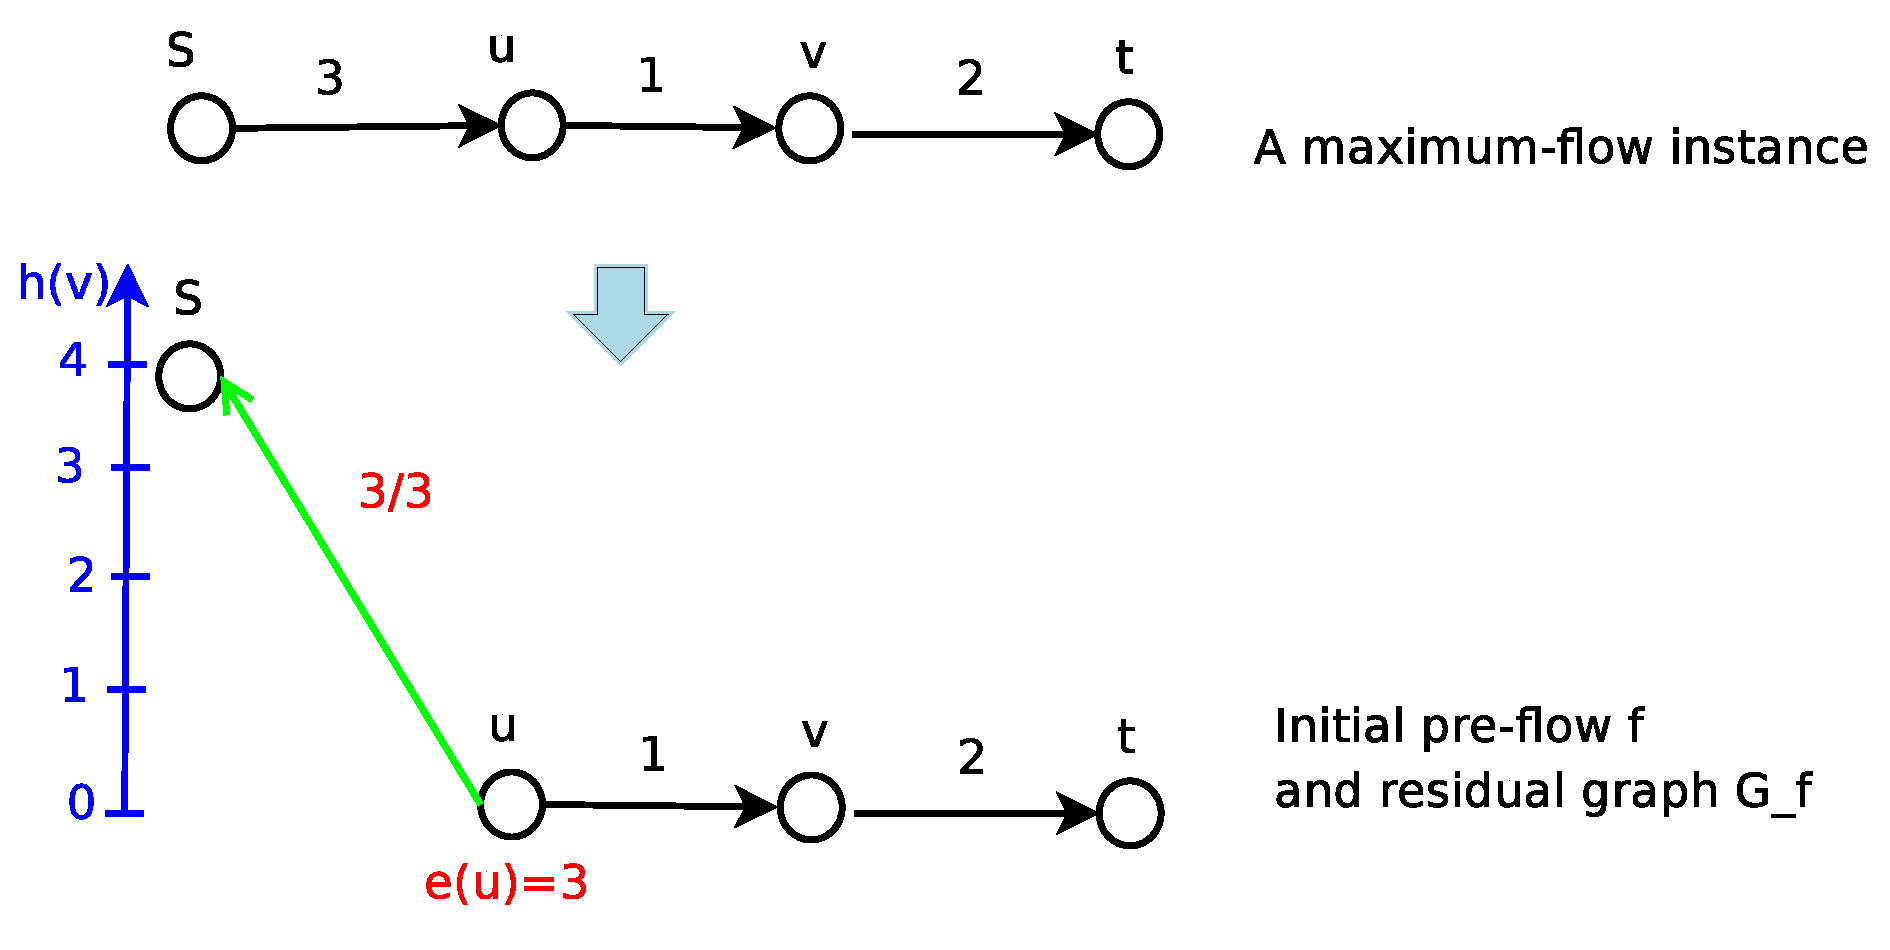
\includegraphics[width=3.2in] {L10-pushrelabelstep0.eps}
  %\caption{Initialization}
  \includegraphics[width=3.2in] {L10-pushrelabelstep1.eps}
  %\caption{Step1}
\end{figure}
\hspace{2cm}初始化\hspace{7cm}Step1
\begin{figure}[H]
  \center
  \includegraphics[width=2.7in] {L10-pushrelabelstep2.eps}
%\caption{Step2}
  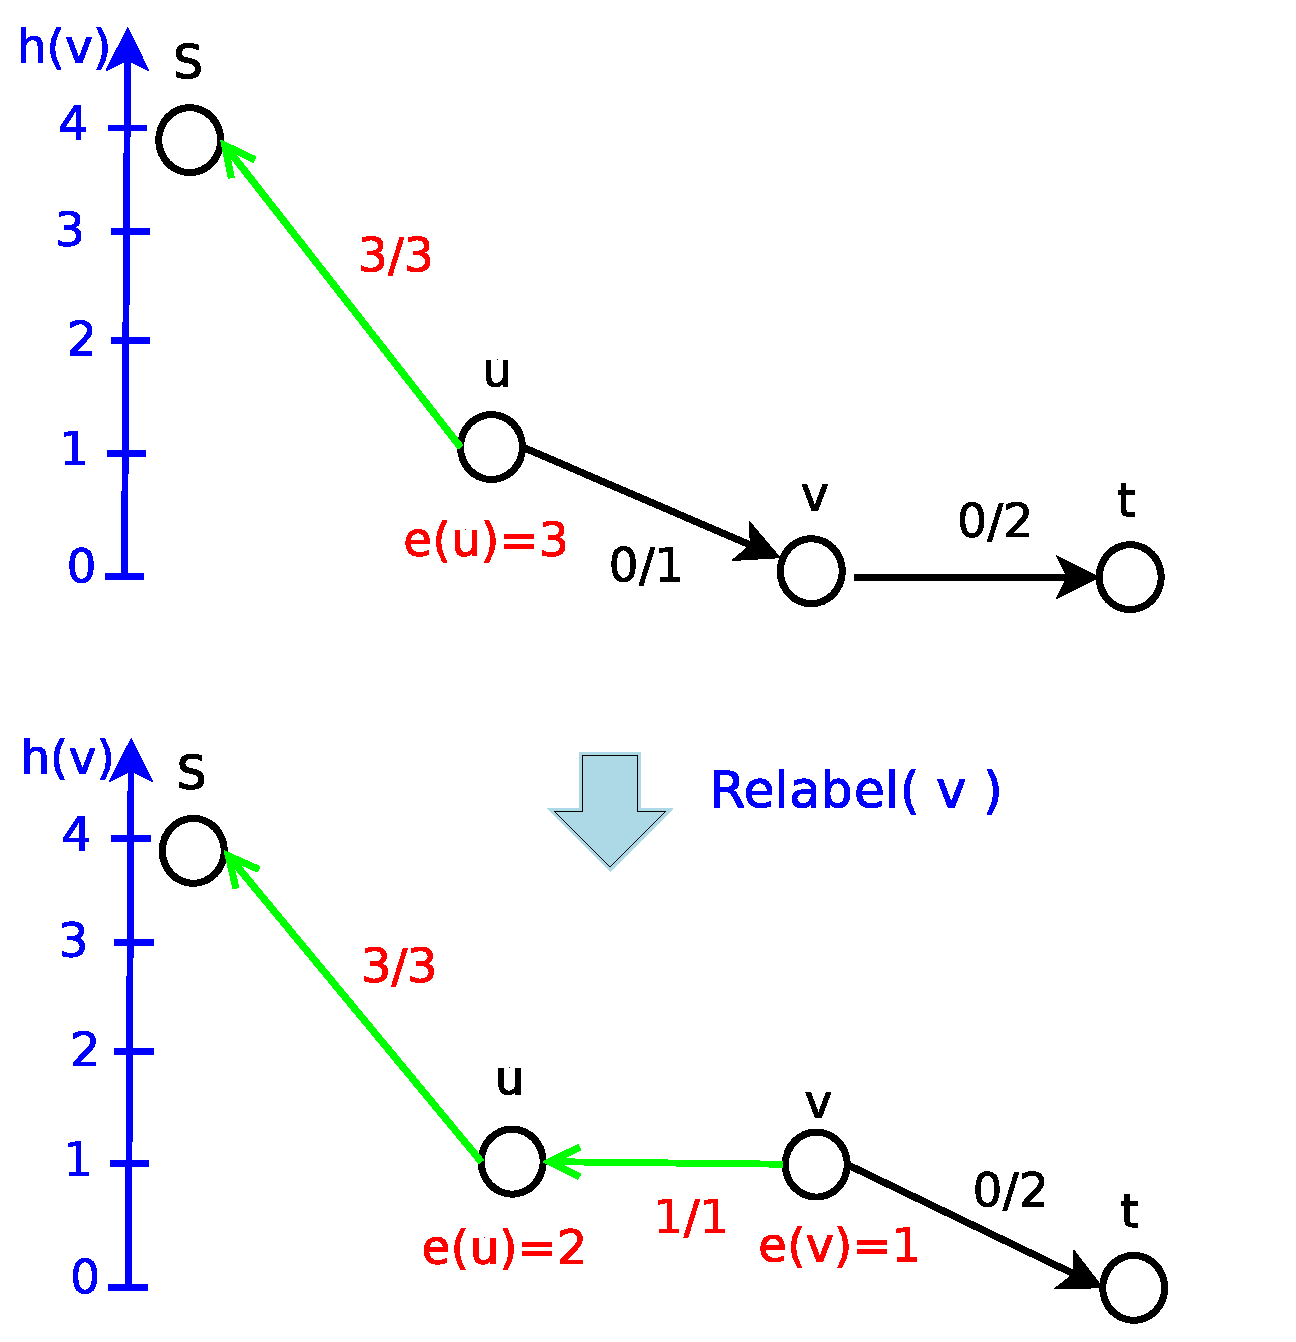
\includegraphics[width=2.7in] {L10-pushrelabelstep3.eps}
%\caption{Step3}
%  \caption{Step2\hspace{5cm}}
\end{figure}
\hspace{3cm}Step2\hspace{7cm}Step3

 \begin{figure}[H]
 \center
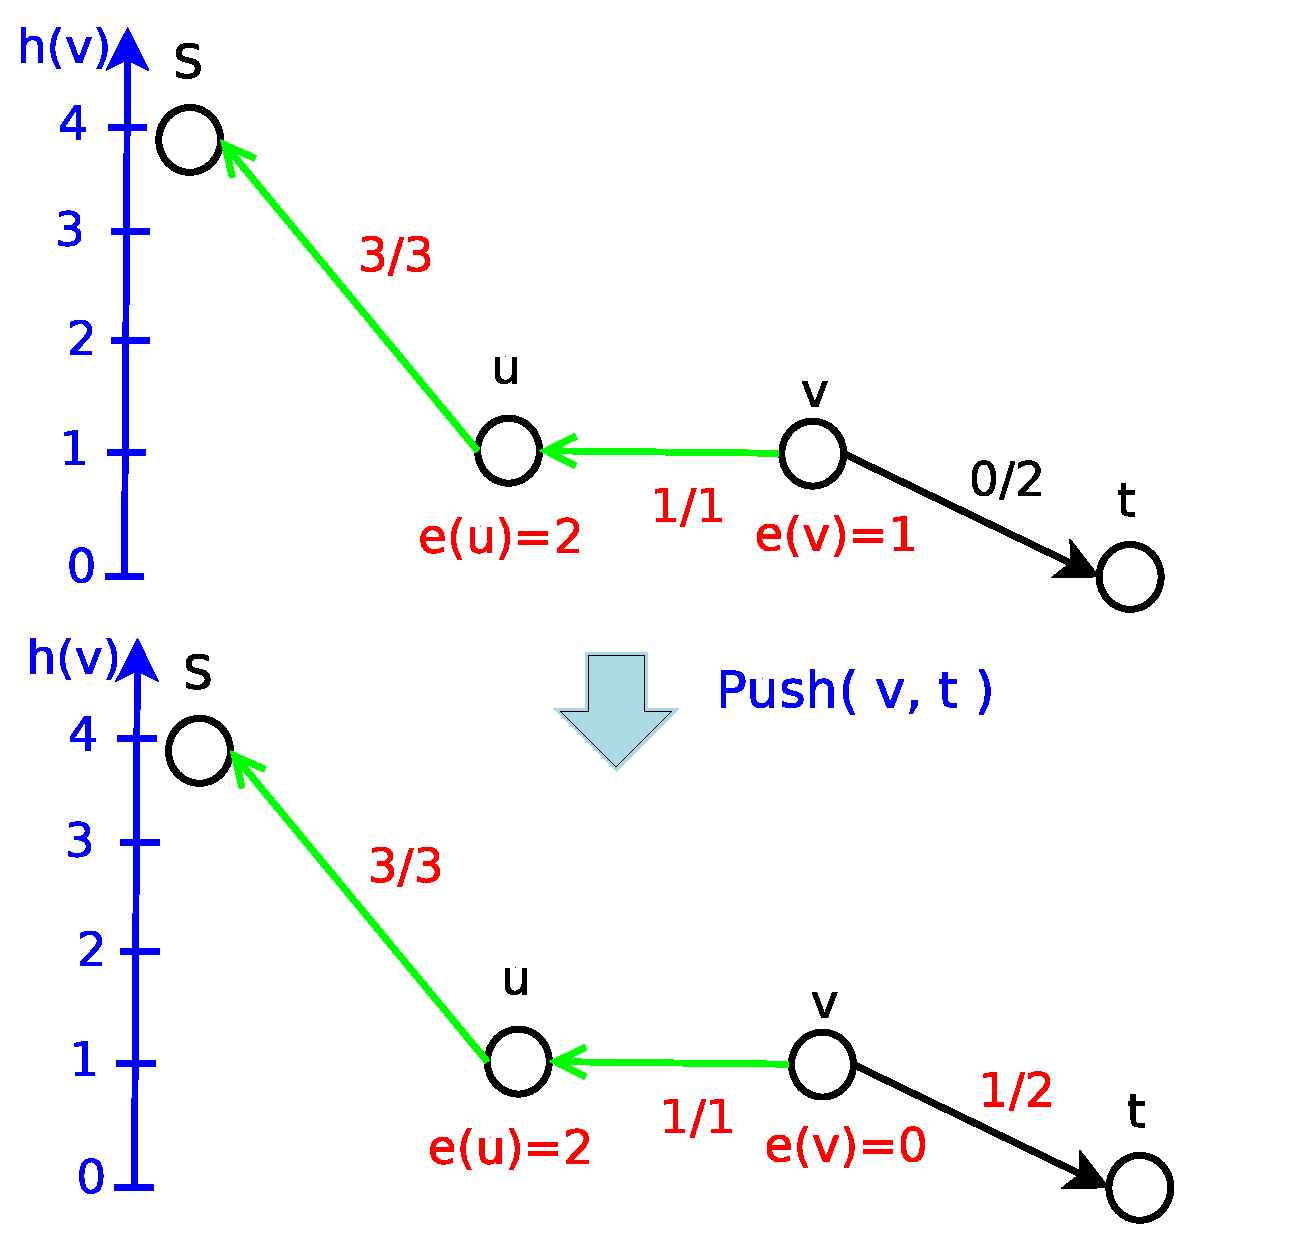
\includegraphics[width=2.7in] {L10-pushrelabelstep4.eps}
  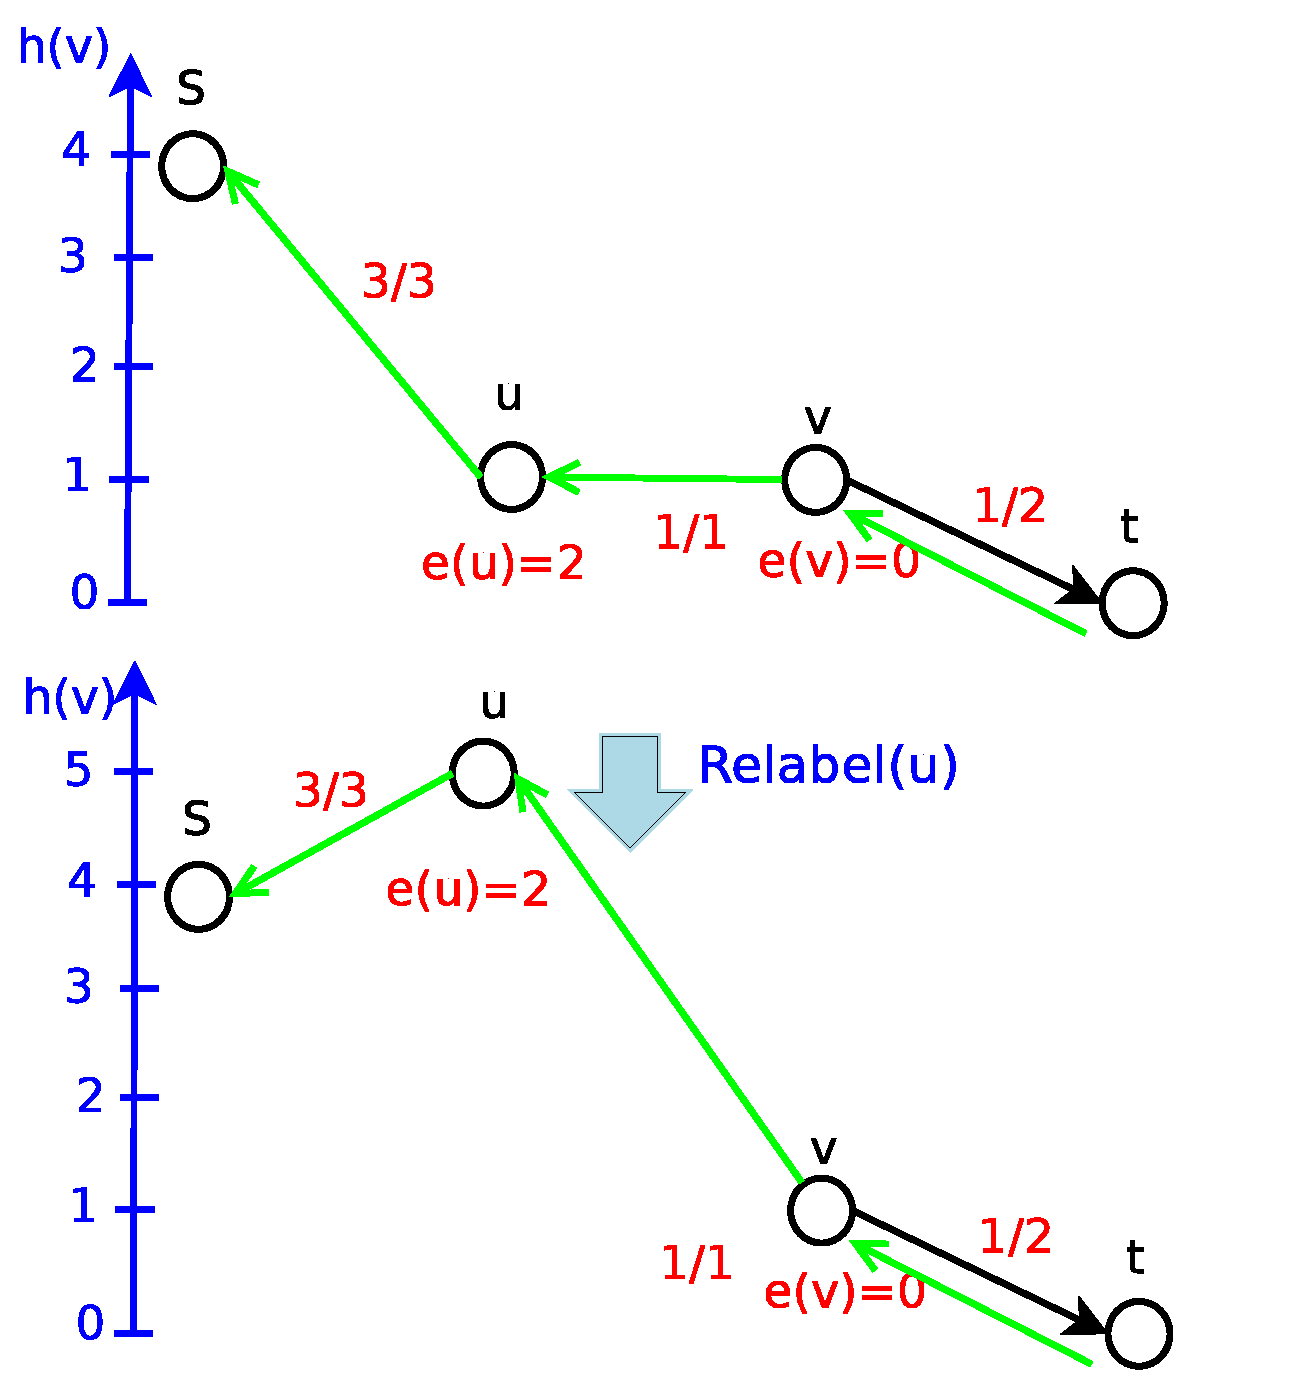
\includegraphics[width=2.7in] {L10-pushrelabelstep5.eps}
%\caption{Step5}
\end{figure}
\hspace{3cm}Step4\hspace{7cm}Step5

\begin{figure}[H]
\center
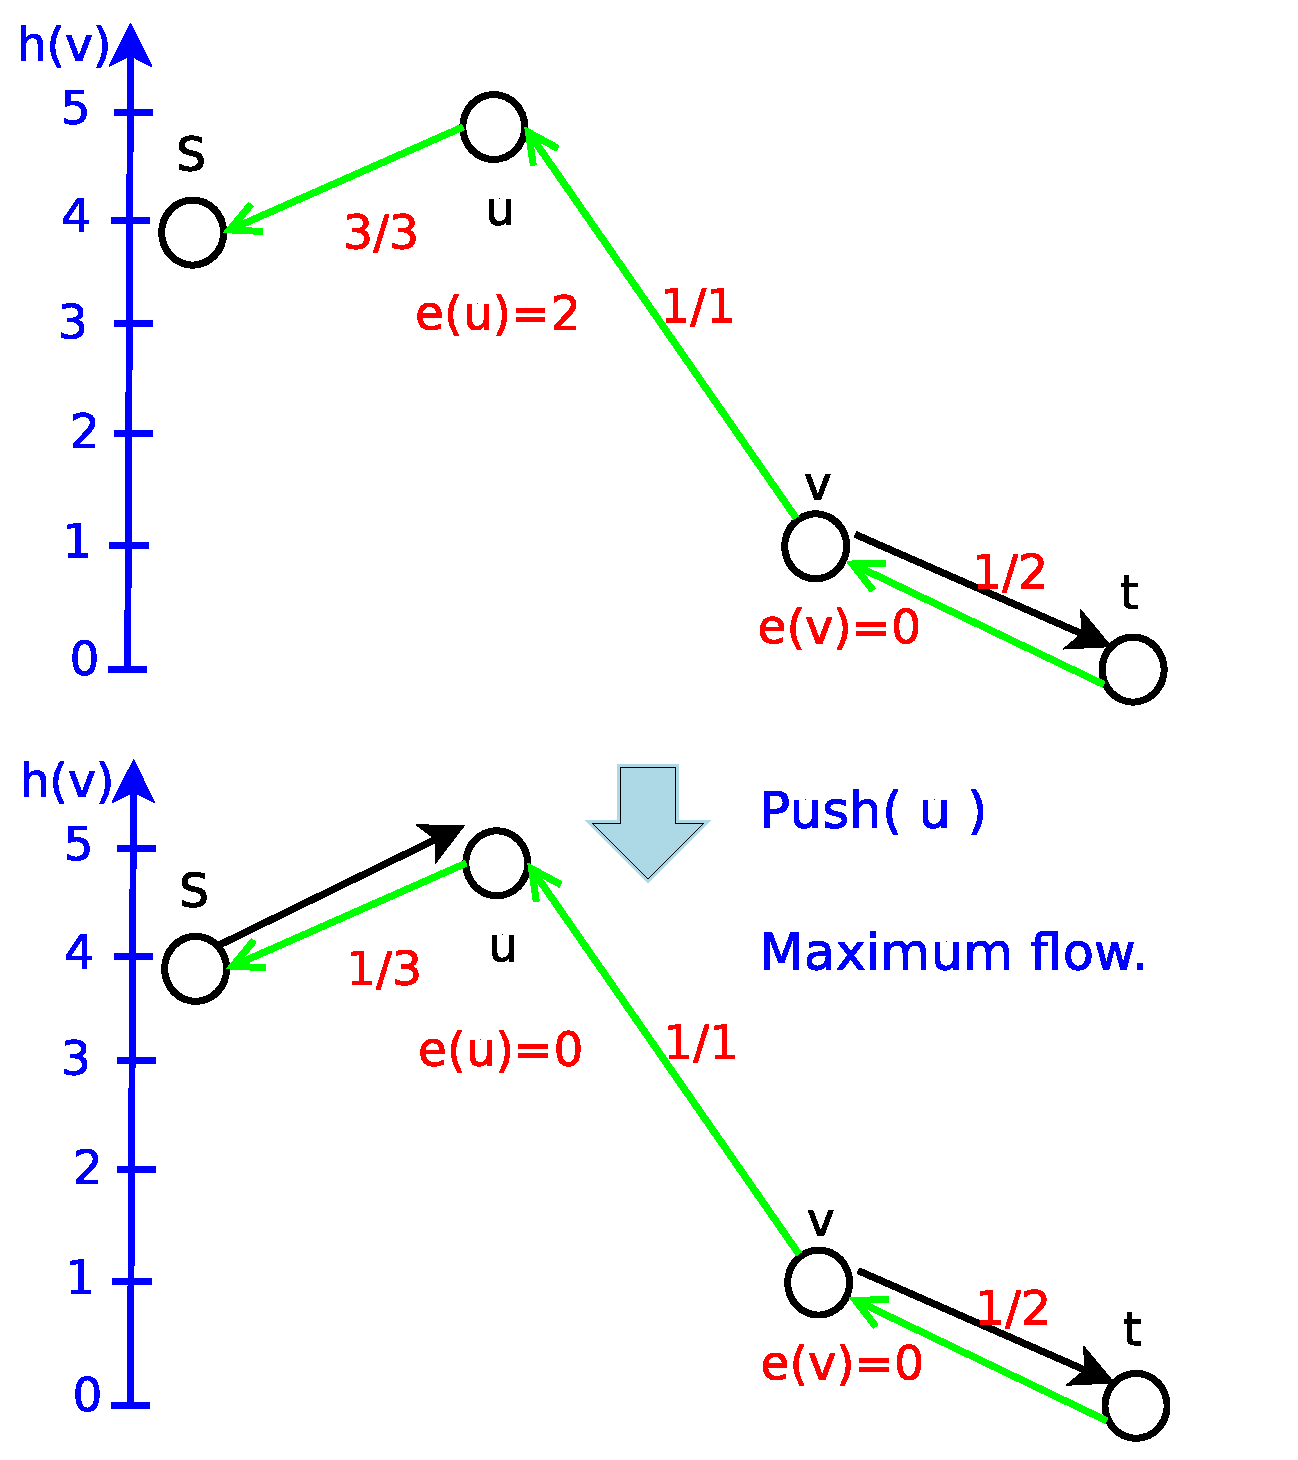
\includegraphics[width=2.7in] {L10-pushrelabelstep6.eps}%\caption{Step6}
\end{figure}
\hspace{8cm}Step6
\subsection{Push-relabel算法实现}
High-level算法:

初始化:
\begin{itemize}
  \item 预流设置:初始时将所有货物均运出,$f(s,u)=C(s,u)$,且对其他边有$f(u,v)=0$。
  \item 标号设置:$h(s)=n$,其他顶点有$h(v)=0$。
\end{itemize}
迭代过程:每一步,对于$E(f)>0$的节点$v$
\begin{itemize}
  \item 若存在一个标号小于$v$的邻居节点$u$,则增加$v$指向$u$的流。
  \item 否则,在标号合理的前提下,增加其高度$h(v)$。
\end{itemize}
Push-relabel algorithm:
  \begin{algorithmic}[1]
    \STATE $h(s) = n; $
    \STATE $h(v) = 0; $ for any $v\neq s$;
    \STATE $f(e) = C(e) $ for all $e=(s,u)$;
    \STATE $f(e) = 0 ;$ for other edges;
    \WHILE{there exists a  node $v$ with $E_f(v) > 0$ }
    \IF { there exists an edge  $(v,w)\in G_f$ s.t. $h(v) > h(w)$; }
    \STATE //Push excess from $v$ to $w$;
    \IF { $(v,w)$ is a forward edge; }
    \STATE $e=(v,w)$;
    \STATE $bottleneck = \min\{ E_f(v), C(e)-f(e) \};$
    \STATE $f(e) += bottleneck;$
    \ELSE
    \STATE $e=(w, v)$;
    \STATE  $bottleneck = \min\{ E_f(v), f(e) \};$
    \STATE $f(e) -= bottleneck;$
    \ENDIF
    \ELSE
    \STATE  $h(v)=h(v)+1;$  //Relabel node $v$;
    \ENDIF
    \ENDWHILE
  \end{algorithmic}

时间复杂度:$T=O(n^2m)$
 % \end{CJK}
